	
\documentclass[11pt,a4paper]{article}

\usepackage[english]{babel}
\usepackage[T1]{fontenc}
\usepackage{lmodern}
\usepackage[a4paper,margin=1in]{geometry}

\usepackage{xcolor}
\usepackage{graphicx}
\usepackage{float}
\usepackage{booktabs}
\usepackage{array}
\usepackage{caption}
\usepackage{subcaption}
\usepackage{tabularx}

\usepackage{amsmath,amssymb,bm}
\usepackage{enumitem}
\usepackage{titlesec}
\usepackage[authoryear]{natbib}
\usepackage{hyperref}
\usepackage{fancyhdr}
\usepackage{pdflscape}
\usepackage{xfrac}
\usepackage{booktabs}
\usepackage{threeparttable}
\usepackage{multirow}
\usepackage{adjustbox}
\usepackage{rotating}
\usepackage{siunitx}


\usepackage{tikz}
\usetikzlibrary{arrows.meta, positioning, shapes.geometric}

\definecolor{darkblue}{rgb}{0,0,0.8}
\hypersetup{
	colorlinks=true,
	citecolor=darkblue,
	linkcolor=darkblue,
	urlcolor=darkblue
}

\setlength{\parskip}{0.55em}
\setlength{\parindent}{0pt}

\title{}
\author{Diego Polanco}
\date{\today}	

\pagebreak
	
\begin{document}
	

%<*ch2body>
\section{Introduction}
\label{ch2:sec:introduction}

Between 1966 and 1970, the profit rate of the United States
non-financial corporate sector fell by 26.9 percent --- and for the
first time in the postwar record, it fell because every channel fell:
demand, distribution, and relational mechanization contracted
simultaneously, with no offsetting force operative in any of them.
This is not a coincidence of cyclical timing. It is the empirical
signature of an accumulation regime that had exhausted the
institutional capacity to contain its constitutive contradictions.

Diagnosing that exhaustion requires a capacity utilization series
whose identification is grounded in something more than a convention:
not the FRB survey (a governance record of capital utilization
reports, not a structural estimate) nor an output-gap measure
(calibration-dependent), but a series derived from the endogenous
relation between mechanization and productivity growth. The
four-channel decomposition this chapter develops turns on that
identification. It separates real capital productivity --- $B_r$,
what the accumulated productive structure can generate per unit of
real capital, conditioned on the quality of mechanization under the
prevailing regime --- from the relative price between aggregate demand
and accumulation demand: $P_Y/P_K$, the terms-of-trade channel
through which world-market price movements enter the profit rate.
When $P_Y/P_K$ contracts sharply --- as it did in 1972--1974 under
the oil shock --- a framework that cannot isolate this channel absorbs
the price movement into the technology reading. Under the
decomposition developed here, the attribution differs substantially:
57.8 percent of the 1972--1974 profit-rate decline belongs to the
price channel, not to any failure of relational mechanization. This
is not a marginal reclassification. It reperiodizes the Fordist
crisis: 1972--1974 was a world-market price event; 1966--1970 ---
simultaneous contraction across every channel, with no institutional
lever capable of relieving more than one pressure at a time --- was
the institutional settlement's structural exhaustion.

The four-channel decomposition presupposes a structurally identified
capacity utilization series. Capacity utilization is not directly
observed in national accounts: it is the demand-side residual that
separates realized output from the productive capacity that capital
accumulation makes available. Identifying it requires a structural
model. This chapter recovers $\hat{\mu}_t$ from the
distribution-conditioned transformation elasticity
$\hat{\theta}(\omega)$ --- extended here through the mechanization
possibility frontier from the scalar identification of the preceding
chapter to its regime-dependent empirical form. At the sample mean
$\bar{\omega} = 0.623$, the US non-financial corporate sector
operated at $\hat{\theta} = 0.918$: in the over-accumulation regime
where capital accumulates faster than productive capacity expands,
with the Fordist wage compromise keeping $\omega_t$ near the
Harrodian knife-edge and regime switching between sub- and
super-Harrodian territory empirically operative across the postwar
cycle.

For Chile, the identification extends the framework to the peripheral
case --- and the extension is a theoretical contribution, not a
sensitivity analysis of the US results. The Chilean economy is not
the US economy operating under different institutional arrangements.
It is a structurally distinct configuration in which the
balance-of-payments constraint enters the mechanization decision
constitutively: higher accumulation demand raises the import bill
for capital goods whose domestic production cannot be substituted
at scale, draining effective demand to capital-goods exporters and
bounding the capacity utilization gains that ISI industrialization
sought to generate. The act of building productive capacity
undermines the demand that would activate it. This structural
contradiction suppresses $\hat{\theta}^{CL}$ below unity throughout
the full ISI arc --- not through a distributional ceiling that policy
could have adjusted, but through the path-dependent interaction
between accumulation demand and the external balance that the
balance-of-payments constraint makes structurally self-reinforcing.
The peripheral transformation elasticity
$\hat{\theta}^{CL}(\omega, s^{ME})$, incorporating
capital-composition heterogeneity and BoP shadow costs, recovers
this configuration directly. The two economies share an analytical
framework; they do not share a dynamic, and the comparison is
organized around the structural object --- relational mechanization
under external constraint --- rather than around US results as a
benchmark from which Chile deviates.

What the MPF identification recovers is not a sharper decomposition
but a different object: capacity utilization with behavioral content,
conditioned on the distribution of the wage share and the quality of
the productive structure accumulated under Fordist regulation. That
series, $\hat{\mu}_t$, rests on a methodological choice that matters
for interpretation --- $\hat{\mu}$ is estimated with gross capital
under Shaikh's GPIM rule (the physical-capacity criterion appropriate
to the labour process), while the profit rate is computed with net
capital at current prices (the monetary-circuit criterion appropriate
to accumulation dynamics). Both stocks are present in US NIPA;
reconciling them is not a data convenience but a reflection of what
gross and net capital measure: the installed productive structure's
capacity to be activated, and the monetary claim accumulated value
makes on that structure. The regulationist reading of the
decomposition that follows does not classify channels --- it reads
them as expressions of the institutional settlement's capacity to
contain its constitutive contradictions. A partial crisis is a swing
resolvable through single-channel institutional adjustment; a
structural crisis is the configuration in which offsetting mechanisms
fail simultaneously and no reconfiguration within the existing regime
is adequate. The Chilean extension is not a robustness check. It is
a structurally distinct case in which the BoP constraint enters the
mechanization decision itself --- making the accumulation regime's
contradictions relational rather than domestic, and the stagnation
tendencies irreducible to the center's institutional logic.

The chapter proceeds as follows. Section~\ref{sec:litreview}
develops the theoretical framework through four strands --- crisis
theory, spatio-temporal fixes, the aggregate crisis trigger, and
the firm-level contradictions of the labour process --- that
converge on the structural identification problem.
Section~\ref{sec:analytical_framework} derives the four-channel
decomposition, the distribution-conditioned MPF, and the causal
inference strategy. Section~\ref{sec:data} describes the US and
Chilean panels. Section~\ref{sec:results} presents the empirical
analysis in two stages for each economy: structural identification
(Stage~A) and profitability decomposition (Stage~B). Appendices
provide full derivations and estimation details.

% =============================================================================
% §2.2 Literature Review: Marxist Crisis Theory and the Role of 
%      Capacity Utilization
% Chapter 2 — Demand-Led Profitability and Structural Crisis of Capitalism
%             in Chile and the United States during the Fordist Era
% Date: 2026-04-04
% Status: Final draft
% =============================================================================

\section{Marxist Crisis Theory and the Role of Capacity Utilization}
\label{sec:litreview}

% ---------------------------------------------------------------------------
\subsection{Re-visiting the History of Crisis Theory}
\label{sec:crisis_limit}

Marxist political economy argues that capitalism is inherently crisis-prone --- 
that the circuit of capital is structurally exposed to interruption because the 
anarchy of production permits no social coordination of aggregate supply and 
demand. \citet{Shaikh1978} provides the seminal reconstruction of this claim 
through a critical history of crisis theories, evaluating the competing 
explanations that the Marxist tradition had generated: underconsumption, 
disproportionality, profit squeeze, and the falling rate of profit. His 
conclusion is that none of these mechanisms is external to capitalism --- each 
arises from the competitive processes constitutive of the mode of production 
itself. The limit of capitalist accumulation is therefore capitalism itself: 
crisis is not a malfunction but a structural property of the system. Demand 
stimulus, in this account, does not resolve crisis but displaces it 
temporally --- deferring the reckoning to a future horizon and enlarging the 
magnitude of the eventual reversal. Critically, Shaikh rejects 
disproportionality as a source of crisis, treating the falling rate of profit 
as the singular tendential law that governs long-run dynamics --- a position 
he maintains through his later work \citep{Shaikh2016}.

\citet{Itoh1978} shares Shaikh's starting point --- crisis arises from the 
competitive processes intrinsic to the capitalist mode of production --- but 
arrives at a more open-ended account. Where Shaikh's history of crisis theory 
converges on a singular tendential law, Itoh distinguishes two qualitatively 
distinct forms of crisis without subordinating one to the other. An 
\textit{excess of capital} crisis (overaccumulation) occurs when capital 
accumulates beyond profitable employment --- the circuit cannot expand fast 
enough to absorb the surplus. An \textit{excess commodity} crisis 
(underconsumption or realization failure) occurs when insufficient aggregate 
demand prevents realization of the produced surplus value. The distinction 
carries a practical consequence that Shaikh's account forecloses: in the 
excess commodity form, demand stimulus may temporarily restore profitability 
by absorbing unrealized output; in the excess of capital form, demand 
stimulus is itself part of the problem, fuelling the overaccumulation that 
will produce a more violent reversal. Capitalism remains crisis-prone in 
both cases, but the mechanisms differ --- and that difference demands a more 
nuanced understanding of \textit{how} the limits of capitalist accumulation 
operate, not merely \textit{that} they exist.

\citet{Arrighi1978} builds on a similar taxonomy of crisis to Itoh's but 
shifts the analytical weight from the forms of crisis to the material 
forces that reshape the terrain of class struggle. His entry point is 
the dynamics of concentration and centralization of capital 
\citep{MarxKVI}: the competitive war among individual capitalists that 
drives expanded reproduction, mergers, and the redistribution of existing 
capital into fewer hands --- processes that accelerate during crisis 
periods as weaker capitalists are overtaken by stronger ones. The 
consequence is not merely falling profitability but a structural 
transformation of the distributive conflict. Higher capital concentration 
increases the collective power of the capitalist class: monopolization 
strengthens price-setting capacity, leverage over suppliers and wages, 
and the ability to react to falling profitability by adjusting idle 
capacities, cutting production, and closing positions. But Arrighi 
identifies a constitutive contradiction within this process. 
Concentration erodes what he calls the \textit{reflexive} strength of 
the working class --- the bargaining leverage derived from tight labour 
markets under dispersed, competitive capital. Yet the same material 
forces that erode reflexive strength simultaneously increase the 
\textit{autonomous} strength of the working class: large-scale production 
concentrates workers, deepens the social division of labour, and creates 
the material conditions for solidarity and collective organization 
\citep[p.~7]{Arrighi1978}.

The process of capitalist restructuring that followed the crises of the 
interwar period was, among other things, an institutional resolution of 
this contradiction. The North-Atlantic Fordist accumulation regime coupled 
mass production with mass consumption under a historical bloc of 
industrialist and working-class consensus at the center of the capitalist 
world system --- developing productive forces through Taylorist work 
organization, productivity-indexed wage relations, and the institutional 
infrastructure of variegated Keynesian national welfare states 
\citep{Vidal2019}. The state absorbed excess capital through unproductive 
expenditures --- military, social reproduction --- while simultaneously 
stabilizing the distributive compromise that Arrighi's dialectic of 
concentration had rendered explosive. The United States led this 
settlement under the umbrella of the Bretton Woods international 
financial architecture, which permitted national policy autonomy 
precisely by constraining cross-border capital mobility. In the global 
south, the relative enclosure of supply chains by Fordist accumulation 
at the center --- the inward orientation of North-Atlantic mass 
production toward North-Atlantic mass consumption --- produced its own 
consequence: import-substitution industrialization strategies pursued 
by Prebischian national developmental states that contested the terms 
of peripheral integration into the world market without breaking from 
it \citep{Prebisch1949, Prebisch1981, Jessop2020}.

\citet{Harvey2001, Harvey2018} provides the conceptual apparatus that 
names what the Fordist settlement was: a \textit{spatio-temporal fix} 
--- crisis displaced across space and deferred through time by means 
of investment in built environments and geographically uneven processes 
of capitalist restructuring. Harvey's spatialization of Marx's 
\textit{Capital} synthesizes three preceding contributions into a 
unified framework. \citet{Luxemburg2015} argued that capitalism cannot 
reproduce itself without non-capitalist peripheries to absorb the 
surplus that the center cannot realize internally --- geographical 
expansion is not incidental but constitutive of accumulation. 
\citet{Trotsky2017} showed that this expansion produces not convergence 
but uneven and combined development: the periphery is integrated into 
the world market on structurally subordinate terms, reproducing rather 
than resolving the contradictions of the center. \citet{Poulantzas2000} 
identified the capitalist state not as an external regulator of this 
process but as a social relation constitutive of it --- crisis management 
through the state is itself a form of the class struggle that 
concentration and centralization intensify. Harvey's three cuts of crisis 
draw these strands together: (i) overaccumulation and underconsumption as 
cyclical phases of the capital circuit; (ii) the credit system bridging 
temporal gaps between production and realization; (iii) geographical 
reallocation displacing crisis to new spaces and future horizons. The 
Fordist accumulation regime constituted, from this perspective, the most 
successful and geographically extensive spatio-temporal fix in the history 
of capitalism --- but one whose spatial architecture simultaneously 
generated the conditions for its contestation from the periphery.

The notion of spatio-temporal fixes maps the geography of crisis displacement with precision. What it leaves open --- and what a complete account of Fordist accumulation requires --- is the mechanism that generates the tendencies being displaced: the variable at the level of accumulation itself whose cumulative path constitutes the trigger, not merely its spatial expression. That question is what the next level of the argument addresses.

% ---------------------------------------------------------------------------
\subsection{Okishio's Crisis Trigger: Cumulative Causation through Capacity Utilization}
\label{sec:okishio}

The classical long-run closure --- the accumulation equilibrium trajectory 
in which realized output matches productive capacity, saving equals 
investment, and the economy reproduces itself smoothly --- is logically 
coherent. \citet{Basu2019} demonstrates its feasibility by establishing 
the proportionality conditions under which Marx's reproduction schemas 
sustain expanded reproduction. But the proof of feasibility does not carry a pattern nor a tendency. \citet{Okishio2022} stresses that the conditions required for smooth 
reproduction are so stringent that decentralized, profit-oriented 
capitalist decision-making cannot sustain them: the accumulation 
equilibrium trajectory is not an attractor but a knife-edge. The 
deviation of actual accumulation from that trajectory is systematically 
self-reinforcing, not self-correcting. Capacity utilization --- the ratio 
of effective output to productive capacity, $\mu_t = Y_t / Y_t^p$ --- is 
the variable that registers this deviation, and its cumulative path is 
what Okishio calls the \textit{crisis trigger}.

Okishio's crisis trigger hypothesis operates through a demand-led causal chain connecting the two Itoh forms. When profit-oriented capitalist behavior drives expansion of productive capacity beyond what effective demand can absorb, $\mu_t$ rises cumulatively---each firm's investment adds capacity that collectively outpaces the growth of realized demand. The overaccumulation builds until inventories accumulate, asset values collapse, and the herd behavior of capitalists simultaneously withdrawing from accumulation produces a violent contraction. This is the \textit{excess of capital} expression: crisis triggered by cumulative overshooting of $\mu_t$ above the accumulation equilibrium trajectory. Conversely, when wage suppression and cost-cutting erode the consumption component of aggregate demand, $\mu_t$ declines secularly---the productive base remains in place but cannot be activated because purchasing power has been systematically compressed. This is the \textit{excess of commodities} expression: a smoother, more protracted realization crisis in which the accumulation equilibrium trajectory recedes as effective demand falls further behind productive capacity secularly \citep{Okishio2022, Itoh1978}.

In both expressions, $\mu_t$ is not an unconstrained parameter. The classical long-run closure requires that effective demand match productive capacity---that the economy reproduce itself smoothly along an \emph{accumulation equilibrium trajectory}. When this closure is imposed, $\mu_t = 1$ by construction and the realization problem disappears. The previous chapter re-interpreted \citet{Shaikh2016}'s methodological proposal for estimating capacity utilization as the estimation of the transformation elasticity of productive capacities to accumulation demand, and the critical replication established that its estimation robustly rejects the assumption of balanced growth in the long run. This chapter lifts the classical long-run closure at $\mu_t=1$, replacing it with a long-run closure of unbalanced growth such that Okishio's equilibrium accumulation trajectory holds only under a full capacity utilization assumption, i.e.\ $\mu_t = 1$. Once smooth reproduction is no longer assumed, $\mu_t$ emerges as the structurally determined gap between effective demand and productive capacities. Identifying the path of capacity utilization, and tracing the causal architecture of Okishio's hypothesis, requires descriptive profitability analysis in conjunction with process tracing and comparative-historical causal inference that isolate the differential dynamics of the underlying components of profitability.



This connects directly to the \citet{Weisskopf1979} decomposition of the profit rate,
\begin{equation}
	r_t = \mu_t \cdot B_t \cdot \pi_t, \label{eq:weisskopf_preview}
\end{equation}
which makes profitability demand-led: $\mu_t$ scales the product of capital productivity at normal capacity $B_t$ and the profit share $\pi_t$. If $\mu_t$ follows a cumulatively unstable path---as the Okishio argument implies whenever the classical long-run closure fails---the profit rate inherits that instability even when $B_t$ and $\pi_t$ are stationary or slowly moving. Reading the Weisskopf decomposition empirically therefore requires a structurally identified $\hat{\mu}_t$---one that is not imposed by a filter or a balanced-growth assumption---which is precisely what the first empirical devleopment of this chapter recovers for the United States and extending also to Chile as an examplary case of peripheral capitalism.

Yet this account of cumulative instability operates at the aggregate level. It shows that $\mu_t$ is structurally unstable without explaining why individual firms cannot coordinate to prevent it. That question descends to the firm itself --- and the firm, as the next section argues, is not the unified decision-body the question presupposes. 


% ---------------------------------------------------------------------------
\subsection{The Firm and Market Anarchy: Multi-Scalar Contradictions Rule Out a Unified Desired Capacity Utilization}
\label{sec:firm_anarchy}

The question of whether firms hold a stable \textit{desired} capacity utilization rate has roots deeper than the Kaleckian model. \citet{Ciccone1986} reconciles the classical tradition of long-period gravitational equilibrium---in which profit rates equalize across sectors at normal capacity---with \citeauthor{Steindl1952}'s \citeyearpar{Steindl1952} insight that firms deliberately maintain spare capacity as a buffer to face demand uncertainty. The normal rate of utilization is, in this account, not an arbitrary convention but a structural feature of competitive capitalist production: it is the utilization rate consistent with the uniform profit rate toward which market prices gravitate. Spare capacity is not waste; it is the form in which firms internalize the anarchic character of market demand.

The canonical Kaleckian model builds on this foundation. Firms set a target utilization rate $\frac{Y^*}{K}$ anchored in the markup and competitive conditions; investment responds to the gap between actual and desired utilization, and the economy settles at the desired rate in the long run \citep{Kalecki1971, Steindl1952, Dutt1990, BhaduriMarglin1990}. A persistent difficulty is that the canonical model cannot reconcile the actual and normal rates in equilibrium---the Harrodian instability problem---which has generated a range of responses: critiques of the investment function's behavioral plausibility \citep{Skott2012}, endogenization of the normal rate so that $\frac{Y^d}{K}$ adjusts to the actual rate \citep{Nikiforos2013, Nikiforos2016, Setterfield2020}, and alternative closures through autonomous demand \citep{Serrano1995}. Despite their differences, these contributions share a common premise: the firm is a sufficiently unified planning subject to hold, pursue, or adjust toward a coherent utilization target. It is this premise that the present chapter challenges.

The challenge operates at two levels. At the macro level, the market is anarchic because social production is not consciously coordinated. No mechanism aggregates the decentralized decisions of individual capitalists into a demand path that would sustain any particular $\mu_t$. This is the Okishio point established in \S\ref{sec:okishio}: the accumulation equilibrium trajectory is a knife-edge, not an attractor.

At the micro level, the firm itself is not a unified decision-body. Following \citet{Vidal2022}, capitalist management confronts two constitutive contradictions of the labour process. The \textit{management contradiction} is the conflict between coordination---organizing production to exploit economies of scope, learning, and flexibility---and discipline---maintaining control over the valorisation process and ensuring that workers produce surplus value. The \textit{workforce contradiction} is the tension between productive socialisation---the development of cooperative capabilities, problem-solving, and engagement---and alienation---the structural exclusion of workers from the purposes and benefits of their own productive activity. Both contradictions pull the utilization decision in incompatible directions: coordination and productive socialisation favour sustained high utilization that develops workers' capacities; discipline and valorisation pressure favour intensification, cost-cutting, and the maintenance of excess capacity as a disciplinary reserve. These pressures operate across incommensurable organizational scales and temporal horizons---from shop-floor struggles over routine, pace, and problem-solving access \citep{Vazquez2006}, through plant-level tactical responses to bottlenecks and product-mix complexity \citep{Anderson2001}, to corporate strategies subordinated to shareholder-value extraction and financialized time horizons \citep{LazonickOsullivan2000}. They do not converge on a single $\frac{Y^d}{K}$. The firm does not overcome market anarchy; it internalizes it through constrained planning shaped by uncertainty and contradictory interests across organizational scales.

If individual firms do not possess coherent utilization targets, the standard aggregation fails at its source. The macro variable e $\frac{Y^d}{K}$ that enters the post-Keynesian investment function has no behavioral referent. What aggregates is not a representative firm's target but the distributive struggle within each firm over how much capacity to activate, under what conditions, and for whose benefit. Aggregate $\mu_t$ is therefore an emergent property of unresolved contradictions interacting through market competition---not a deviation from a well-defined center of gravity.

The exhaustion of the Fordist settlement was not an exogenous shock but 
the product of its own contradictions. The Taylorist labour process that 
had sustained the settlement rested on what \citet{Braverman1998} 
diagnosed as the systematic separation of conception from execution --- 
the degradation of work into deskilled, routinized tasks under 
managerial control. \citet{Vidal2022} shows that this diagnosis, while 
correct on the discipline side, is one-sided: the same deskilling that 
secured managerial control simultaneously eroded the cooperative and 
cognitive capacities on which production depended, generating a 
contradiction within management itself that Braverman's framework could 
not register. As competitive pressures shifted the basis of efficiency 
toward economies of scope and flexibility, the Taylorist suppression of 
worker cognition became not a source of stability but a fetter on 
accumulation. At the aggregate level, the full-employment conditions 
that the Fordist settlement had achieved --- most decisively in the 
United States through Vietnam War military spending \citep{Baker1996} 
--- produced the very forces that undermined it. Near-full employment 
tightened labour markets, raised wages, 
strengthened the working class's bargaining position and militancy intensity. However, 
these gains  came at the cost of falling profitability: what the decomposition records as a declining $\hat{\mu}_t$ through
the mid-1960s is not, under this reading, a failure of demand management
but the political-economic contradiction of a settlement that could not
simultaneously sustain full employment, rising real wages, and adequate
profit rates. The crisis of Fordism was, in this sense, the crisis of the
political economy of full employment itself.

% ---------------------------------------------------------------------------
\subsection{Synthesis: A Multi-Level Theory of the Crisis Trigger}
\label{sec:synthesis}

The four strands of the preceding analysis produce not a catalogue of 
crisis theories but a coherent ladder --- each level specifying a 
distinct mechanism, each necessary but insufficient on its own.

\begin{table}[h]
	\centering
	\caption{Multi-scalar theory of the crisis}
	\label{tab:crisis_ladder}
	\begin{tabular}{p{3.5cm} p{6.5cm} p{4cm}}
		\toprule
		\textbf{Level} & \textbf{Mechanism} & \textbf{Reference} \\
		\midrule
		Mode of production & Crisis is endemic; demand stimulus displaces, 
		not resolves & \citet{Shaikh1978}; \citet{Itoh1978} \\
		Meso/spatial & Spatio-temporal fixes displace crisis across scales, 
		time and spaces & \citet{Arrighi1978}; \citet{Harvey2001, Harvey2018} \\
		Aggregate/macro & $\mu_t$ path is the crisis trigger; cumulative 
		disequilibrium & \citet{Okishio2022} \\
		Firm/organizational & Multi-scalar contradictions rule out a stable 
		desired utilization rate & \citet{Vidal2022} \\
		\bottomrule
	\end{tabular}
\end{table}

An accumulation regime that suppresses the crisis trigger must operate across all four levels simultaneously. The multi-level typology establishes this as a structural claim: crisis is not an aberration from a normally functioning capitalism but the form taken by the exhaustion of a specific institutional configuration that was never a resolution of its constitutive contradictions. What the typology cannot do is identify empirically which channel carries the dominant stagnation tendency in any given period, or whether capitalist investment responds to each channel symmetrically. The classification grid is conceptually exact but empirically silent---structural identification of $\mu_t$ is the precondition for making it speak.


\section{Analytical Framework}
\label{sec:analytical_framework}

The profit rate compresses three objects of interest for political 
economy --- demand conditions ($\mu$), the structural character of the 
production regime ($B$), and the distributional outcome of class 
struggle ($\pi$) --- into a single observable but decomposable 
magnitude. Profitability analysis decomposes it; the laws of 
accounting guarantee the decomposition is exact. But accounting 
decomposition alone does not answer the behavioral question: how do 
capitalists respond to each component when deciding how much surplus 
to reinvest? The analytical framework of this chapter reconciles 
both --- leveraging the distinction between profitability (what the 
accounting identity reveals) and recapitalization (what capitalists 
do with what it reveals) --- so that the behavioral content of the 
underlying drivers of profitability can be structurally identified.

The framework has three layers. First, as established in Chapter~1, the measurement of capacity utilization identifies a non-observed component in its denominator through a Johansen VECM \citep{Johansen1991}: a system identification in which speed-of-adjustment coefficients reveal which variables are structurally endogenous to the long-run relation and which are weakly exogenous. Second, the chapter revisits the accounting identity that separates the three channels underlying profitability dynamics, and motivates why the fully disaggregated four-channel specification --- separating real capital productivity from the relative price of capital goods --- is the primary object of interest. Third, it recovers the causal architecture of the Fordist settlement through a combination of within-case process tracing \citep{Collier2011}, cross-case small-$N$ causal inference \citep{Mahoney2000}, and comparative-historical relational analysis \citep{Mahoney2004}: the decomposition provides the outcome signatures; the causal method identifies the mechanisms that produced them.

\subsection{Stagnation and Crisis: A Typology}
\label{subsec:typology}

\citet{Basu2019} classifies crisis expressions by the relation between 
surplus-value production and its realization conditions, and by whether 
the source of disruption operates through the demand side or the 
financial side. Each cell corresponds to a directional movement in one 
or more of $\mu_t$, $B_t$, $\pi_t$ --- the channels that Layer~1 
separates.

\begin{table}[htbp]
	\centering
	\caption{Surplus-value accounting grid}
	\label{tab:basu_grid}
	{\small
		\begin{tabular}{lll}
			\toprule
			& \textit{Excess of surplus value} 
			& \textit{Deficit of surplus value} \\
			\midrule
			Demand side    & Underconsumption / realization crisis 
			& Profit squeeze (rising labor strength) \\
			Financial side & Financial fragility                   
			& Falling (normal) rate of profit \\
			\bottomrule
	\end{tabular}}
\end{table}

The grid does not assign causation. It classifies the form in which 
accumulation-regime incoherence registers in the profit-rate 
components --- a classification that presupposes the separability 
of channels. Redefined in the terms of \citet{Vidal2014}, each cell 
becomes a form of regime dysfunctionality --- a configuration in 
which the institutional settlement can no longer contain the 
contradiction it was built to manage. This licenses reading multiple 
\textit{offsetting} stagnation tendencies within a single regime 
period as dysfunctionality rather than equilibrium. Three categories 
formalize the distinction \citep{Vidal2014, Vidal2019}: 
\textit{stagnation tendency} --- downward pressure on profitability 
operative through one or more channels but not yet producing an 
interruption of the circuit; \textit{partial crisis} --- interruption 
resolvable by partial reconfiguration of the institutional settlement; 
\textit{structural crisis} --- deep and prolonged interruption 
requiring drastic restructuring of the accumulation regime.


\begin{table}[htbp]
	\centering
	\caption{Stagnation and crisis categories}
	\label{tab:vidal_categories}
	{\small
		\begin{tabular}{ll}
			\toprule
			Category & Definition \\
			\midrule
			Stagnation tendency & Downward pressure on profitability; does not interrupt the circuit \\
			Partial crisis      & Interruption resolvable by partial institutional reconfiguration \\
			Structural crisis   & Deep, prolonged interruption requiring drastic restructuring \\
			\bottomrule
	\end{tabular}}
\end{table}

The grid establishes that different crisis expressions leave distinct signatures in $(\mu_t, B_t, \pi_t)$---and that tendencies can coexist and offset within a single regime period, producing apparent stability that conceals accumulating dysfunctionality. What the grid cannot establish is the relative weight of each channel in any historically specific conjuncture, because $\mu_t$ and $B_t$ are not independently observable in national accounts. The channel decomposition presupposes a structurally identified capacity utilization series; without it, the grid assigns form without measure.


\subsection{Profitability Analysis}
\label{subsec:profitability_analysis}

The profit rate over non-residential capital decomposes exactly into 
three multiplicative factors \citep{Weisskopf1979}:
\begin{equation}
	r \equiv \frac{\Pi}{K} 
	= \frac{Y}{Y^p}\cdot\frac{Y^p}{K}\cdot\frac{\Pi}{Y} 
	= \mu \cdot B \cdot \pi
	\label{eq:weisskopf}
\end{equation}

\begin{table}[htbp]
	\centering
	\small
	\caption{Weisskopf decomposition for Profitability Analysis}
	\label{tab:weisskopf_factors}
	\begin{tabular}{llll}
			\toprule
			Variable & Representation & Definition & Channel \\
			\midrule
			Capacity utilization  & $\mu$  & $Y/Y^p$  & Demand\\
			Capital productivity  & $B$    & $Y^p/K$  & Technology\\
			Profit share          & $\pi$  & $\Pi/Y$  & Distribution\\
			\bottomrule
	\end{tabular}
\end{table}

Effective profitability is demand-led: $r = \mu \times r^n$, where $r^n \equiv B\pi$
is normal-capacity profitability. Capitalists signal from realized $r$, not from
$r^n$---the demand channel activates or suppresses the structural and distributive
channels through $\mu$ \citep{BleckerSetterfield2019}. 

The \citet{Weisskopf1979} decomposition extends directly into the investment
decisions. Define the gross accumulation rate $g_K \equiv I/K$, and the recapitalization
rate $\chi \equiv I/\Pi$---the share of profits that capitalists direct back into
accumulation rather than consumption. Since $r = \mu B \pi$, the identity yields:
%
\begin{equation}
	\label{eq:accumulation_identity}
	g_K = \chi \cdot \pi \cdot \mu \cdot B
\end{equation}

The gross accumulation identity nests the Weisskopf decomposition:
\begin{align}
	g_K \equiv \frac{I}{K}
	&= \frac{I}{\Pi}\cdot\frac{\Pi}{Y}\cdot\frac{Y}{Y^p}\cdot\frac{Y^p}{K} \\
	&= \chi \cdot \pi \cdot \mu \cdot B
\end{align}

Since $r = \pi\mu B$, the identity can be written as:
\begin{equation}
	g_K = \chi\, r - \delta
	\label{eq:accum_compact}
\end{equation}

The three channels are  distinct by accounting; they should therefore enter the investment  function separately by default. Compressing $\mu$ and $B$ into 
capital productivity yields the Bhaduri-Marglin specification; 
compressing all three into the profit rate yields the 
Kaldor-Robinson specification. Both are parametric restrictions on 
the fully disaggregated specification, which enters $\pi$, $\mu$, 
and $B$ separately. The disaggregation is empirically feasible only 
because $\hat{\mu}_t$ and $\hat{B}_t$ are structurally identified objects.



\subsection{Causal Inference Strategy}
\label{subsec:causal_inference}

The accounting decomposition identifies the channels through which the
profit rate moved; it cannot by itself identify why it moved through
those channels. The causal architecture of the Fordist settlement ---
why demand activation dominated over distribution and technology as
the mechanism counteracting over-accumulation, and why the same
mechanism became the primary vector of structural crisis when it
failed --- requires a causal inference strategy that operates on the
decomposition as its outcome variable.

This chapter deploys three complementary methods. Within-case
process tracing \citep{Collier2011} identifies observable implications
of the proposed causal mechanism at each profit-rate swing: if demand
activation was the institutional containment mechanism, then
single-channel contractions in the functional period should be
concentrated in $\mu_t$; multi-channel contractions that include
$\mu_t$ should be disproportionately deep; and the 1966--1970 episode
should uniquely exhibit simultaneous contraction across all three
channels with demand as the dominant weight. The channel decomposition
provides the temporal ordering and mechanism signatures required for
this inference. Cross-case small-$N$ causal analysis
\citep{Mahoney2000} evaluates whether the structural conditions
identified for the US case operate as necessary conditions in the
Chilean case: if BoP-binding is a sufficient condition for
transforming the technological stagnation tendency into a structural
crisis, then the Chilean trajectory should exhibit the escalation
sequence --- mechanization trap → financial fragility → external
crisis --- independently of the distributional channel. Comparative-historical
relational analysis \citep{Mahoney2004} places both cases within the
world-system articulation through Bretton Woods: the gold-dollar
standard creates asymmetric exposure to the $P_Y/P_K$ shock (one-sided
for the US, two-sided for Chile), which means the 1972--1974 episode
is not two instances of the same event but one world-monetary event
with structurally differentiated effects.

The accounting floor argument establishes the benchmark. The log-linearized
accumulation identity is exact:
%
\begin{equation}
	\label{eq:log_identity}
	\ln g_K = \ln \chi + \ln \pi + \ln \mu + \ln B
\end{equation}

When the recapitalization rate $\chi$ is constant, the identity
imposes unit elasticity on every channel: $\beta_j = 1$ for all $j$.
Unit elasticities are not a behavioral claim --- they are what the
identity delivers when recapitalization does not respond to
conditions. Every measured departure from unity is behavioral content,
directly attributable to the institutional structure that governed
recapitalization decisions in each regime period \citep{Vidal2013,
Vidal2019}. The specifications of profitability models nest as
restrictions on this baseline, following \citet{Basu2017}: the
Robinson-Keynes model imposes $\eta_j = 0$ for all $j$; the
Bhaduri-Marglin type imposes $\eta_3 = 0$; the fully disaggregated
Foley-Michl type allows all $\beta_j$ free. The comparative-historical
method identifies which specification is consistent with the observable
implications of the proposed causal mechanism in each case --- not by
estimating the investment function as a stand-alone regression, but by
reading the decomposition through the causal lens.


\subsection{Structural Identification of the Transformation Elasticity}
\label{sec:theta_identification}

The accounting foundation separates three channels but does not yet
identify them empirically. The profit rate decomposition $r = \mu
\cdot B \cdot \pi$ presupposes that $\mu_t$ and $B_t$ can be
observed independently --- but neither is directly measured in
national accounts. What is observed is output ($Y_t$), capital
($K_t$), and the wage share ($\omega_t$). The transformation
elasticity $\theta$ --- how capital converts into productive
capacity --- mediates between the observed and the unobserved.
Identifying $\theta$ is therefore the precondition for recovering
$\mu_t$ and $B_t$ as structurally distinct objects.

The identification proceeds from a cost-minimization problem on the
mechanization possibility frontier. Capitalists minimize the unit
cost of mechanization net of productivity gains, at normal capacity
and given distribution:
%
\begin{equation}
	\min_{\hat{q}} \; c = (1-\omega)\hat{q} - \hat{a}
	\quad \text{s.t.} \quad
	\hat{a} = \lambda_1 \hat{q} + \lambda_2 \hat{q}^2,
	\qquad \lambda_1 > 0, \; \lambda_2 < 0
	\label{eq:cost_min}
\end{equation}
%
where $\hat{q}$ is the rate of mechanization, $\hat{a}$ is labour
productivity growth, $(1-\omega)$ is the profit share --- the
distributive cost of mechanization --- and the quadratic frontier
imposes diminishing returns ($\lambda_2 < 0$). The first-order
condition yields:
%
\begin{equation}
	\hat{q}^*(\omega) = \frac{(1-\omega) - \lambda_1}{2\lambda_2}
	\label{eq:foc_qstar}
\end{equation}

The transformation elasticity evaluated at the optimum is the ratio
of average to marginal productivity on the frontier:
%
\begin{equation}
	\boxed{\theta(\omega) = \frac{\hat{a}^*}{\hat{q}^*}
	= \lambda_1 + \lambda_2 \hat{q}^*
	= \frac{\lambda_1 + (1 - \omega)}{2}}
	\label{eq:theta_omega}
\end{equation}
%
$\theta$ is linear in the wage share. The curvature of the frontier
($\lambda_2$) determines the optimal mechanization rate but drops out
of the ratio --- the transformation elasticity depends only on the
MPF slope ($\lambda_1$) and the distributional outcome ($\omega$).

The capacity equation in logs, $y_t^p = \theta_t k_t$, combined with
$\mu_t = Y_t / Y_t^p$ and the linearity of $\theta$ in $\omega$,
produces the cointegrating relation that Stage~A estimates:
%
\begin{equation}
	y_t = c + \beta_1 k_t + \beta_2 (\omega_t \cdot k_t) + \xi_t
	\label{eq:coint}
\end{equation}
%
where $\beta_1 = (1+\lambda_1)/2$, $\beta_2 = -1/2$, and
$\xi_t = \ln \hat{\mu}_t$. The endogenous transformation elasticity
is $\hat{\theta}_t = \hat{\beta}_1 + \hat{\beta}_2 \omega_t$. The
residual $\xi_t$ is structurally identified capacity utilization ---
not a statistical residual but the demand-side content that the
accounting identity and the cost-minimization FOC jointly pin down.

Three restrictions follow from the derivation:

\begin{enumerate}
	\item[\textbf{R1.}] $\beta_2 = -1/2$ --- the identifying restriction
	from the quadratic MPF. A favourable test would check assuming a 
	quadratic shape of the mechanization function. 
	\item[\textbf{R2.}] $\beta_1 > 1$ --- admissibility condition
	guaranteeing that mechanization is profitable
	($\lambda_1 > 1 - \omega$).
	\item[\textbf{R3.}] The wage share $\omega_t$ enters the
	cointegrating relation only through the interaction
	$\omega_t k_t$, not as a standalone level. Distribution
	affects capacity through its interaction with the capital
	stock, not independently.
\end{enumerate}

R1, R2, R3 are tested jointly within the Johansen VECM framework procedure
\citep{Johansen1991}, as restricted specification of the VECM model against the pseudo-unrestricted identification\footnote{I refer to "pseudo-unrestricted" identification of a VECM model, because given the interactive variables included in the state-vector of the system, their short-run representation both in the autoregresive and the error correction matrices are excluded. Their inclusion entails non-sensical short-run structural dynamics, which is developed in more detail in the appendix \S \ref{app:us_stage_a}.} If the restrictions are not rejected, validates the underlying assumption of a non-linear structure of the mechanization function of labour productivity, as well as the feasibility of magnitude orders at a given range of distributive variables in the observed sample. Nevertheless, these restrictions does not entail the order of magnitude under which the endogenous $\theta(\omega)$ will be identified as time varying due its distributive dependence.

An important qualification concerns the inclusion of variables that are already \(I(0)\)  in the level vector of a Johansen system. Their presence does not, by itself, invalidate estimation. However, if an \(I(0)\) variable is allowed to enter the cointegrating vector unrestrictedly, part of the stationary space may be generated mechanically by that variable’s own order of integration rather than by a genuine long-run relation among the \(I(1)\) variables. In that case, the estimated rank may no longer admit a clean interpretation as the dimension of a shared long-run constraint among common stochastic trends. For this reason, clearly stationary variables are usually better treated as conditioning variables, deterministic controls, or short-run regressors unless theory specifically requires their restricted appearance in the long-run relation. In the present framework, where the cointegrating vector is interpreted as the long-run transformation linking accumulation to productive capacity, preserving that interpretation requires not necessarily dropping \(I(0)\) from being excluded of the long-run matrix \(\beta\) \citep{ReinselVelChen2022}.

An important limitation of an unbalanced growth closure to identify productive capacities $g_Y^p=\theta(\omega) \, g_K$ relying on a system co-integration methodology is that operates in rates of growth, not in levels. Hence, it requires only one period assumption of capacity utilization level, or assuming a year of operation at full capacity utilization. For the case of the United States was considered  an approximate level of the average measure of capacity utilization during the 1948 pinned at 80\%. 


% =============================================================================
% §2.3.X+1 — Chilean Extension: Two Types of Capital
% Position: follows the US identification subsection
% =============================================================================
% ============================================================
% §3.5 Peripheral Extension: Capital Composition and
%       BoP-Constrained Identification
% VERSION: corrected 2026-04-07
% CHANGES FROM ORIGINAL:
%   C1 — eq:cl:theta_hat: corrected formula using s_ME
%   C2 — eq:cl:regime_indicator: lambda → gamma (notation fix)
%   C3 — eq:cl:state_vector_imports: renamed duplicate label
%   C4 — §subsec:chile_imports paragraph: ζ₁/ζ₂ corrected
%   C5 — eq:cl:capital_decomp: footnote on phi vs s_ME added
%   P1 — §subsec:chile_imports opening: prose cleanup
%   T1 — Two typos fixed
% ============================================================

\subsection{Peripheral Extension: Capital Composition and
	BoP-Constrained Identification}
\label{subsec:theta_identification_chile}

The center identification recovers $\hat{\theta}(\omega_t)$ from a
single cost-minimization problem on a homogeneous capital stock. In
peripheral capitalism, this architecture is insufficient. The
heterogeneity of capital stock imposes an external restriction due to
the import requirements of machinery and equipment ($K^{ME}$), while
assuming that non-residential infrastructure ($K^{NR}$) is domestically
producible but tied to accumulation of machinery and equipment at a
given choice of technique under cost-minimizing principles. Because the
domestic capital-goods sector cannot substitute for imported machinery
at scale, the mechanization decision is constrained by the availability
of foreign exchange. The balance-of-payments constraint enters the
cost-minimization problem through the import content of machinery
investment.

\subsubsection{Capital Decomposition and the Peripheral MPF}
\label{subsec:chile_mpf}

Define the capital stock decomposition:
%
\begin{equation}
	K^{CL} = K^{NR} + K^{ME},
	\qquad
	\phi_t \equiv \frac{K_t^{ME}}{K_t^{CL}} \in (0,1),
	\label{eq:cl:capital_decomp}
\end{equation}
%
where $\phi_t$ is the machinery share of the total non-residential
capital stock.\footnote{In the empirical implementation, the theoretical $\phi_t$ is
	computed as $s_t^{ME} \equiv K_t^{ME}/(K_t^{NR}+K_t^{ME})$, which is
	equivalent to $K_t^{ME}/K_t^{CL}$ under the decomposition
	$K^{CL} = K^{NR} + K^{ME}$. The bounded share $s_t^{ME} \in (0,1)$
	ranges from 0.25 to 0.75 in the Chilean panel; its ISI-period mean
	is 0.302 and its neoliberal-period mean is 0.543.}
The import content of machinery investment in the early period of
interest was registered by \citet{Kaldor1959} at $\xi \approx 0.92$--$0.94$.

Infrastructure and machinery carry differential productivity effects.
Define the composition-weighted MPF slope:
%
\begin{equation}
	\bar{\psi}(\phi)
	=
	\psi^{NR}(1-\phi)+\psi^{ME}\phi,
	\label{eq:cl:psi_bar}
\end{equation}
%
The inequality $\psi^{ME} > \psi^{NR}$ is the structural content of
the \citet{Kaldor1959} hypothesis: embodied technical change is higher
in imported machinery than in domestic infrastructure. Higher $\phi$
raises productivity potential but deepens import dependence.
The peripheral MPF is:
%
\begin{equation}
	\hat{a}
	=
	\bar{\psi}(\phi)\,\hat{q}
	+
	\lambda_2\,\hat{q}^{\,2},
	\qquad
	\lambda_2 < 0,
	\label{eq:cl:mpf}
\end{equation}
%
same functional form as the center \eqref{eq:cost_min} but with a
composition-dependent slope.

\subsubsection{The BoP Penalty and the Effective Profit Share}
\label{subsec:chile_bop_penalty}

Mechanization at rate $\hat{q}$ generates an import bill
$\xi\,\phi\,\hat{q}\,K^{CL}$. Let $\lambda \geq 0$ denote the
shadow cost of foreign exchange --- the scarcity rent under the
BoP constraint. The peripheral cost-minimization problem is:
%
\begin{align}
	\min_{\hat{q}}\; c^{CL}
	&=
	(1-\omega)\hat{q}
	-
	\hat{a}
	+
	\lambda\,\xi\,\phi\,\hat{q}
	\label{eq:cl:cost_min}
	\\[4pt]
	\text{s.t.}\qquad
	\hat{a}
	&=
	\bar{\psi}(\phi)\,\hat{q}
	+
	\lambda_2\,\hat{q}^{\,2},
	\qquad
	\lambda_2<0.
	\label{eq:cl:mpf_constraint}
\end{align}
%
The first-order condition yields:
%
\begin{equation}
	\hat{q}^{CL*}(\omega,\phi,\lambda)
	=
	\frac{(1-\omega)-\lambda\,\xi\,\phi-\bar{\psi}(\phi)}
	{2\lambda_2},
	\label{eq:cl:foc_qstar}
\end{equation}
%
and the peripheral transformation elasticity:
%
\begin{equation}
	\boxed{
		\theta^{CL}(\omega,\phi,\lambda)
		=
		\frac{\bar{\psi}(\phi)+\pi^{eff}}{2},
		\qquad
		\pi^{eff}
		\equiv
		(1-\omega)-\lambda\,\xi\,\phi
	}
	\label{eq:cl:theta}
\end{equation}
%
The BoP constraint compresses the effective profit share available for
mechanization. For given $\omega$, the periphery achieves a lower
$\theta$ than the center by exactly $\lambda\xi\phi/2$. The center
solution is recovered as the special case $\lambda = 0$, $\phi = 0$.

Comparing with the center \eqref{eq:foc_qstar}:
%
\begin{equation}
	\hat{q}^{US*} - \hat{q}^{CL*}
	=
	\frac{
		\lambda\,\xi\,\phi
		+
		\left[\bar{\psi}(\phi)-\psi_1\right]
	}{
		2|\lambda_2|
	}
	>
	0.
	\label{eq:cl:q_gap}
\end{equation}
%
The gap has two sources: the BoP penalty $\lambda\xi\phi$ and the
structural MPF slope differential $\bar{\psi}(\phi)-\psi_1$.

\subsubsection{Regime Switch from Complementary Slackness}
\label{subsec:chile_regimes}

The BoP ceiling $\bar{\phi}$ limits the machinery share in new
investment. By complementary slackness, two regimes emerge:
%
\begin{center}
	\begin{tabular}{llll}
		\toprule
		& $\lambda$ & $\phi_{new}$ & $\theta$ \\
		\midrule
		Regime~1 (BoP slack)   & $= 0$ & $= \phi^*$            & $\theta^{(1)}$ \\
		Regime~2 (BoP binding) & $> 0$ & $= \bar{\phi} < \phi^*$
		& $\theta^{(2)} < \theta^{(1)}$ \\
		\bottomrule
	\end{tabular}
\end{center}
%
The gap between regimes decomposes as:
%
\begin{equation}
	\theta^{(1)}-\theta^{(2)}
	=
	\underbrace{
		(\psi^{ME}-\psi^{NR})(\phi^*-\bar{\phi})
	}_{\text{composition compression}}
	+
	\underbrace{
		\frac{\lambda\,\xi\,\bar{\phi}}{2}
	}_{\text{forex shadow cost}}.
	\label{eq:cl:theta_gap}
\end{equation}
%
The ceiling $\bar{\phi}$ responds to the non-reinvested surplus ---
profits not converted into machinery investment. \citet{Kaldor1959}
identifies two competing forces through which this surplus conditions
the foreign-exchange constraint: lower machinery investment reduces
current demand for imported capital goods, relaxing the ceiling; yet
surplus flowing into capitalist consumption tightens it, since luxury
consumption carries substantially higher import content than average
consumption once invisible imports are accounted for. Whether the
accumulation-relief or the consumption-drain mechanism dominates is
historically contingent and empirically recovered from the long-run
import propensity relation
%
\begin{equation}
	m_t
	=
	\zeta_0
	+
	\zeta_1\, k_t^{ME}
	+
	\zeta_2\, nrs_t
	+
	\zeta_3\, \omega_t
	+
	ECT_{m,t},
	\label{eq:cl:imports_coint}
\end{equation}
%
where $m_t$ and $nrs_t$ are imports and non-reinvested surplus in log
levels, $\zeta_1 > 0$ captures the structural import demand generated
by machinery accumulation, $\zeta_2 \gtrless 0$ recovers the net
distributional effect of the non-reinvested surplus without sign
restriction, and $ECT_{m,t}$ represents structural imbalances that are
introduced below as the regime-switching variable for the identification
of sudden shifts in the dynamics of unbalanced growth.

\subsubsection{First Stage: Cointegration System for Propensity to Import}
\label{subsec:chile_imports}

% C3: label renamed from eq:cl:state_vector_theta to eq:cl:state_vector_imports
% P1: opening prose cleaned up
% C4: ζ₁/ζ₂ descriptions corrected; jargon lock applied (no channel labels)
% T1: typos fixed

The first stage identifies the long-run import propensity through a
cointegration system on the state vector:
%
\begin{equation}
	Y_t
	=
	\left(
	m_t,\;
	k_t^{ME},\;
	nrs_t,\;
	\omega_t
	\right)',
	\label{eq:cl:state_vector_imports}
\end{equation}
%
Theoretically, $\zeta_1 > 0$ captures the structural import demand
generated by machinery accumulation --- each unit of capital deepening
raises the structural import requirement --- while $\zeta_2 \gtrless 0$
recovers the net effect of the non-reinvested surplus on the
foreign-exchange constraint without sign restriction, and $\zeta_3$
identifies the distributional channel through which the wage share
compresses or amplifies import demand \citep{Kaldor1959}. The estimated
disequilibrium term $ECT_{m,t}$ summarizes the externally driven
systemic imbalances arising from the scarcity of foreign exchange and
its allocation between capital-goods imports and surplus-financed
consumption.

\subsubsection{Second Stage: Threshold VECM for the Productive Frontier}
\label{subsec:chile_frontier_threshold}

The state vector for the productive frontier is:
%
\begin{equation}
	X_t^{CL,\theta}
	=
	\left(
	y_t,\;
	k_t^{NR},\;
	k_t^{ME},\;
	\omega_t k_t^{ME}
	\right)',
	\label{eq:cl:state_vector_frontier}
\end{equation}
%
The interaction term is $\omega_t k_t^{ME}$ because the
cost-minimization problem shows that distribution conditions technique
choice through the machinery component specifically. Infrastructure is
distribution-insensitive at business-cycle frequency.

The first cointegrating vector identifies the capacity frontier:
%
\begin{equation}
	y_t
	=
	\kappa_1
	+
	\theta_0\, k_t^{NR}
	+
	\psi\, k_t^{ME}
	+
	\theta_2\,(\omega_t k_t^{ME})
	+
	ECT_{\theta,t},
	\label{eq:cl:cv1}
\end{equation}
%
where $\psi = \psi^{ME}-\psi^{NR}$ is the machinery productivity
premium and $\theta_2 < 0$ is the distribution-composition interaction.

This frontier relation does not directly identify the level of capacity
utilization. The term $ECT_{\theta,t}$ is a long-run disequilibrium
term of the frontier system. It identifies deviations between realized
output and the productive-capacity frontier implied by capital
composition and distributional conditions, but it does not, by itself,
identify the level of $\mu_t^{CL}$.

% C1: theta^CL formula corrected
% Old: θ̂^CL(ω,φ) = θ₀ + ψ·φ + θ₂·ω·φ  [WRONG — φ unbounded]
% New: θ̂^CL(ω,s_ME) = θ₀(1−s_ME) + (ψ+θ₂ω)·s_ME  [FOC-consistent derivative]

The empirical transformation elasticity is recovered from the frontier
coefficients as the derivative of productive capacity with respect to
total log-capital $k_t^{CL} = \ln(K_t^{NR}+K_t^{ME})$:
%
\begin{equation}
	\boxed{
		\hat{\theta}^{CL}(\omega_t,\, s_t^{ME})
		=
		\hat{\theta}_0\,(1-s_t^{ME})
		+
		\left(\hat{\psi} + \hat{\theta}_2\,\omega_t\right)s_t^{ME}
	}
	\label{eq:cl:theta_hat}
\end{equation}
%
where $s_t^{ME} \equiv K_t^{ME}/(K_t^{NR}+K_t^{ME}) \in (0,1)$ is the
bounded machinery composition share --- the empirical counterpart of
the theoretical $\phi_t$ in \eqref{eq:cl:capital_decomp}. This
expression is the exact partial derivative $\partial y^p/\partial k^{CL}$
evaluated at the estimated frontier coefficients, and is the empirical
counterpart of \eqref{eq:cl:theta}.

% C2: lambda → gamma in regime indicator
% Old: R_t = 1[ECT_m,t-1 > λ]  [λ collision with shadow price]
% New: R_t = 1[ECT_m,t-1 > γ]  [γ = threshold estimand]

To identify nonlinear external activation, the productive frontier is
estimated as a threshold VECM in the sense of \citet{Seo2006}, using
the first-stage external disequilibrium as the transition object. Let
the regime indicator be
%
\begin{equation}
	R_t
	=
	\mathbf{1}\!\left[\widehat{ECT}_{m,t-1} > \gamma\right],
	\label{eq:cl:regime_indicator}
\end{equation}
%
where $\gamma$ is the threshold parameter estimated by conditional
least squares (CLS), and its activation identifies the periods in which
$\lambda > 0$ --- the shadow price on the BoP constraint becomes
operative and compresses the feasible mechanization path.

The threshold VECM is then
%
\begin{equation}
	\Delta X_t^{CL,\theta}
	=
	\mu
	+
	\alpha^{(1)} ECT_{\theta,t-1}(1-R_t)
	+
	\alpha^{(2)} ECT_{\theta,t-1}R_t
	+
	\sum_{j=1}^{p}\Gamma_j \Delta X_{t-j}^{CL,\theta}
	+
	\varepsilon_t,
	\label{eq:cl:tvecm_theta}
\end{equation}
%
where the threshold effect is driven by the estimated external
disequilibrium recovered from the first-stage import system. In this
architecture, the threshold is not imposed on the import-propensity
equation itself. Rather, the import system identifies the external
imbalance, and the threshold VECM identifies how that imbalance
activates the shadow-price effect on the machinery-sensitive productive
frontier.

Productive-capacity growth is then constructed through the closure
%
\begin{equation}
	g_{Y_t^{p,CL}}
	=
	\hat{\theta}^{CL}(\omega_t,\, s_t^{ME})\,g_{K_t^{CL}},
	\label{eq:cl:frontier_growth}
\end{equation}
%
so that the method identifies the evolution of utilization only in
growth rates:
%
\begin{equation}
	g_{\hat{\mu}_t^{CL}}
	=
	g_{Y_t^{CL}}
	-
	g_{Y_t^{p,CL}},
	\label{eq:cl:mu_growth}
\end{equation}
%
The level of $\hat{\mu}_t^{CL}$ is recovered only after imposing a
pin-year normalization:
%
\begin{equation}
	\hat{\mu}_{t_0}^{CL}
	=
	\mu_0,
	\label{eq:cl:mu_pin}
\end{equation}
%
and accumulating the productive-capacity series forward and backward
from $t_0$.

\subsubsection{Recursive Identification}
\label{subsec:chile_recursive}

The recursive architecture is therefore clear. In a first stage, a
cointegration system for propensity to import is estimated, and its
estimated parameters and estimated disequilibrium term summarize the
externally driven systemic imbalances. In a second stage, a threshold
VECM for the productive frontier is estimated, using those first-stage
estimations to identify $\gamma$ as the threshold at which the shadow
price $\lambda$ on the external constraint activates, compressing the
machinery-sensitive transformation of accumulation into productive
capacity. The frontier system therefore identifies the evolution of
capacity utilization only up to a normalization, while the threshold
activation identifies the foreign-exchange penalty that compresses the
feasible mechanization path. The two systems are brought together in
interpretation through the theoretical object
$\theta^{CL}(\omega_t,\phi_t,\lambda)$ and its empirical counterpart
\eqref{eq:cl:theta_hat}.


%%%%%%%%%%%%  Section Data and Measurement #############

\section{Data and Measurement}
\label{sec:data}

The empirical framework developed in the preceding sections calls for real output, productive capital stocks, and distributional variables for both the United States and Chile. Before describing each panel, we set out two measurement principles that govern their construction.

The first is dual capital accounting. Productive capacity and value advanced are distinct theoretical objects and must be measured accordingly. The state variable $k_t$ entering the VECM is the log of the \emph{gross} real capital stock, constructed under the Gross Physical Investment Method \cite[Appendix on Ch.~6]{Shaikh2016}. Depreciation does not instantaneously extinguish a machine's contribution to productive capacities, so gross measures of capital stocks---not net---are the appropriate empirical counterpart for their estimation under an unbalanced growth closure. Using net stocks in the would conflate the depreciation regime with the transformation elasticity $\hat{\theta}$, biasing the structural parameter and contaminating the recovered utilization series $\hat{\mu}_t$. The profit rate denominator, by contrast, requires capital valued at current reproduction cost: we use the net current-cost stock $K^N_{\text{cc},t}$. Chapter~1 defends this dual convention at length; here we simply apply it.

Notice that \citet{Shaikh2016} strongly emphasizes on avoidiing relative prices issues by scaling with by a common deflator. I decide not doing so and face the potential bias by omission of the price index, because precisely if that bias tanslate to the estimates of $\theta(\omega)$  it would be capturing implicitly components of unbalanced growth and interdepartamental disproportionality. Both conventions are consistent with the New Interpretation of the transformation problem of value to prices \citep{Foley1982,Basu2022}, under which the monetary expression of labor time mediates between value and price magnitudes at each period without the contradictions of the standard transformation procedure. I adopt current-cost valuation with the exception of the treatment of physical cuantities for the estimation of capacity utilization is developed at done at real prices of 2024, the last year in the sample. 

\subsection{United States}
\label{sec:data:us}

The US panel comprises 96 annual observations spanning 1929--2024. It is an original dataset assembled programmatically from the Bureau of Economic Analysis (BEA) and Federal Reserve Economic Data (FRED) APIs. The pipeline fetches raw National Income and Product Accounts (NIPA) income and Fixed Asset Tables, constructs non-financial (NF) sector aggregates, and applies the GPIM to produce capital stock series that remain stock-flow consistent. Because the pipeline draws directly from the API, the entire panel can be regenerated against any future BEA data vintage without manual intervention.

A deliberate sectoral boundary governs the panel. Pairing corporate profit shares with aggregate GDP and total private capital---as is common in much of the empirical literature---introduces an accounting inconsistency at the NF sector margin. I avoid this by constructing all variables within the same NF boundary: output is gross value added, the profit share $\pi_t$ is the ratio of gross operating surplus to gross value added, only net of employment compensation, the capacity state variable is gross capital stock derived under \citet{Shaikh2016} GPIM rules using a Weibull retirement function with asset $K^G_t$ from Fixed Asset Table~4.1 (retirement distribution formalization and parameter decisions in Appendix~\ref{app:ret_distribution}), and the profit rate denominator is $K^N_{\text{cc},t}$.

Two estimation windows structure the empirical work. Stage~A --- capacity utilization identification via the Johansen VECM --- exploits the full 1929--2024 sample; this long span is feasible because the cointegration procedure requires only real quantity series, not deflated price data. Stage~B --- profitability decomposition --- restricts attention to the post-WWII deflator-reliable period, with the Fordist window (1944--1973) as the primary estimation interval, which makes it possible to read the channel decomposition against the institutional periodization of the US accumulation regime. 

\subsection{Chile}
\label{sec:data:cl}

The Chilean panel on capital stocks spans 1900--2025 and represents a novel harmonization of multiple historical and contemporary sources. No single existing dataset provides the asset-level, stock-flow consistent capital stocks that the GPIM framework demands, so we constructed one. The resulting harmonization builds gross and net stocks separately for machinery and equipment (ME) and non-residential construction (NRC) from 1900 to 2024 under the GPIM rules, reconciling three secondary sources with seminal accounts on investment and capital accumulation studies in Chile and Latin America: i) \citet{Hofman2000} provides 1900-1994 series of gross fixed capital formation for the period 1900-1994 in constant 1980~CLP; ii) \citet{PerezEyzaguirre2019} doctoral dissertation provides the most comprehensive data on historical national accounts for Chile, a contribution that built upon the first major effort by the Clio-Lab by the Catholic University compiled by \citet{Luders2016}. 

The contribution of \citet{PerezEyzaguirre2019} relies on new archival and national accounts reconciliation, which adjusts the series first presented by \citet{Luders2016} across multiple windows of historical statistics. Alike Clio-Lab data set his revision of the data set is presented in real terms at 2003 CLP prices. Precisely because \citet{PerezEyzaguirre2019} presents the most comprehensive and coherent data on aggregate demand conciliated with value added at sectoral level, our harmonization of capital stocks uses his data as the anchor for stock-flow consistency and implementation of GPIM rules to estimate gross and net capital stocks for accounts of non-residential, residential, machinery and equipment, and non-residential infrastructure capital stocks; iii) to extend the series to contemporary period, the harmonization of capital stocks splices with the longest series of Chile's Central Bank. To my knowledge, no comparable GPIM-consistent, asset-disaggregated capital stock series exists for Chile over this time horizon. The harmonization pipeline records full provenance; all methodological decisions are documented in a repository for future release with a companion dataset paper that goes beyond the scope of this chapter. 

The backbone of the panel is \citet{PerezEyzaguirre2019}'s stock-flow consistent national accounts (1860--2010, constant 2003 prices), which disaggregate FBKF into machinery and equipment and infrastructure. \citet{Hofman2000} series provides separation of gross fixed capital formation for the residential and non residential sector. Historical price deflators come from ClioLab (base $2003=100$) and are extended forward from 2011 with BCCh deflators rebased to 2003, spliced at 2010. A wald test for the two-sample $t$-tests on growth rates across all six deflator pairs in the 1996--2010 overlap window confirm no statistically significant difference ($p \gg 0.05$ in every case), validating the splice. For the capacity utilization window, real quantities are extended to 2025 using BCCh national accounts on a 2018 base, chain-linked to 2003 prices; continuity at the 2010--2011 junction is exact (0.0\% deviation). The investment deflator $P^K_t$ is constructed as a ratio of nominal to real FBKF from ClioLab for 1940--2010, chained forward with the ratio growth rates for 2010--2025. Current-cost net stocks follow as $K^N_{\text{cc},t} = K^N_t \times P^K_t / 100$. Distributional variables---the wage share $\omega_t$ and profit share $\pi_t$---draw on \citet{Astorga2023} for 1920--2010, spliced with BCCh income accounts through 2024 and satisfying exact distributive consistency ($\pi_t + \omega_t = 1$).

The Fordist analysis window (1940--1973) has complete coverage on all key variables. The periodization reflects Chile's specific rhythm of industrialization within the world-system hierarchy rather than a mechanical transposition of US dates: ISI strategies were set in motion in Latin America before US Fordism consolidated as a global accumulation regime, and the 1973 terminal date marks the co-constitutive retreat of import-substitution industrialization and the onset of neoliberal counter-revolution. Post-1973 observations are retained in both panels for the capacity utilization sample, enabling rolling-window robustness exercises. The Fordist profitability window begins in 1940 because no source provides price indexes for capital stocks or investment flows before that year --- a constraint that excludes the 1932--1939 ISI consolidation phase, but does not affect the analytical core of the identification, which is anchored in the 1940--1973 arc. 

\section{Results}
\label{sec:results}

\subsection{United States}
\label{sec:results_us}
%% ===========================================================================
%% §2.8.1 — US Results: Stage A (MPF and Capacity Utilization)
%% File: sec_results_us_stage_a.tex
%% Input into main document via \input{sec_results_us_stage_a}
%% Cross-references appendix labels from appendix_us_stage_a.tex
%% ===========================================================================

\subsubsection{Stage A: The Mechanization Possibility Frontier}
\label{sec:results_us:stage_a}

% ---- Lead with central result -----------------------------------------------

The Johansen reduced-rank regression on the state vector
$X_t = (y_t, k_t, \omega_t, \omega_t k_t)'$ with $K = 2$ lags over
1929--2024 identifies a single dominant cointegrating relation with
overwhelming statistical support (trace statistic $= 159.26$, 5\%
critical value $= 53.12$; Appendix~\ref{app:sa:rank}). The
$y$-normalized first eigenvector recovers the MPF:
%
\begin{equation}
	y_t = 8.924\, k_t + 222.161\, \omega_t
	- 12.851\, \omega_t k_t - 138.254
	\label{eq:mpf_us}
\end{equation}
%
from which the distribution-conditioned transformation elasticity is:
%
\begin{equation}
	\boxed{\hat{\theta}(\omega_t) = 8.924 - 12.851\,\omega_t}
	\label{eq:theta_us}
\end{equation}

% ---- Structural interpretation -----------------------------------------------

The sign $\partial\hat{\theta}/\partial\omega = -12.851 < 0$ confirms the
FOC-grounded theoretical restriction developed in
Section~\ref{sec:analytical_framework}: a higher wage share reduces the
transformation elasticity with which capital is converted into productive
capacity. At the sample mean $\bar{\omega} = 0.623$, the estimated
elasticity is $\hat{\theta} = 0.918$\footnote{Evaluated as
	$8.924 - 12.851 \times 0.623 = 0.918$; the difference from rounding
	the intermediate product to three decimal places is 0.003 and is
	analytically inconsequential.} --- the economy operates, on average,
in an over-accumulation regime where the productive capacity frontier
grows \emph{slower} than the capital stock.\footnote{Full parameter
	estimates, standard errors, and structural roles are reported in
	Table~\ref{tab:sa:cv1_params} (Appendix~\ref{app:sa:cv1}).}

% ---- Regime partition -------------------------------------------------------

The Harrodian knife-edge --- the wage share at which $\hat{\theta} = 1$
and productive capacity grows at the same rate as capital --- obtains at:
%
\begin{equation}
	\omega_H = \frac{8.924 - 1}{12.851} = 0.617
	\label{eq:omega_H_us}
\end{equation}
%
This threshold lies inside the observed sample ($\omega_t \in [0.540,
0.682]$), confirming that regime switching between sub-Harrodian and
super-Harrodian dynamics is empirically operative in the US non-financial
corporate sector. The crisis boundary $\omega^* = 0.694$
($\hat{\theta} = 0$) lies outside the sample --- the economy never reaches
the structural collapse threshold
(Appendix~\ref{app:sa:regime}).\footnote{The restricted specification
	$(\omega = 0, \omega k = 1/2)$ is statistically accepted but compresses
	$\hat{\theta}$ into a narrow super-Harrodian band $[1.48, 1.54]$ that
	eliminates regime switching. Since $\omega_H$ inside the sample is
	required by the theoretical framework, the unrestricted specification is
	preferred. See Appendix~\ref{app:sa:restrictions}.}

Figure~\ref{fig:theta_omega_scatter} displays the MPF schedule in
$(\omega, \hat{\theta})$ space. The regime partition is visible in the
period coloring: Fordist observations (1945--1973) cluster near the
knife-edge $\omega_H$, while Post-Fordist observations (1974--2024) are
concentrated in sub-Harrodian territory ($\hat{\theta} < 1$) as the
secular decline in the wage share pushes the economy persistently toward
a regime in which capital accumulates faster than productive capacity
expands --- the structural expression of the over-accumulation stagnation
tendency whose institutional management the remainder of this analysis traces.

\begin{figure}[htbp]
	\centering
		\caption{The Mechanization Possibility Frontier: $\hat{\theta}(\omega_t)$,
		US Non-Financial Corporate Sector, 1929--2024.}
	\label{fig:theta_omega_scatter}
	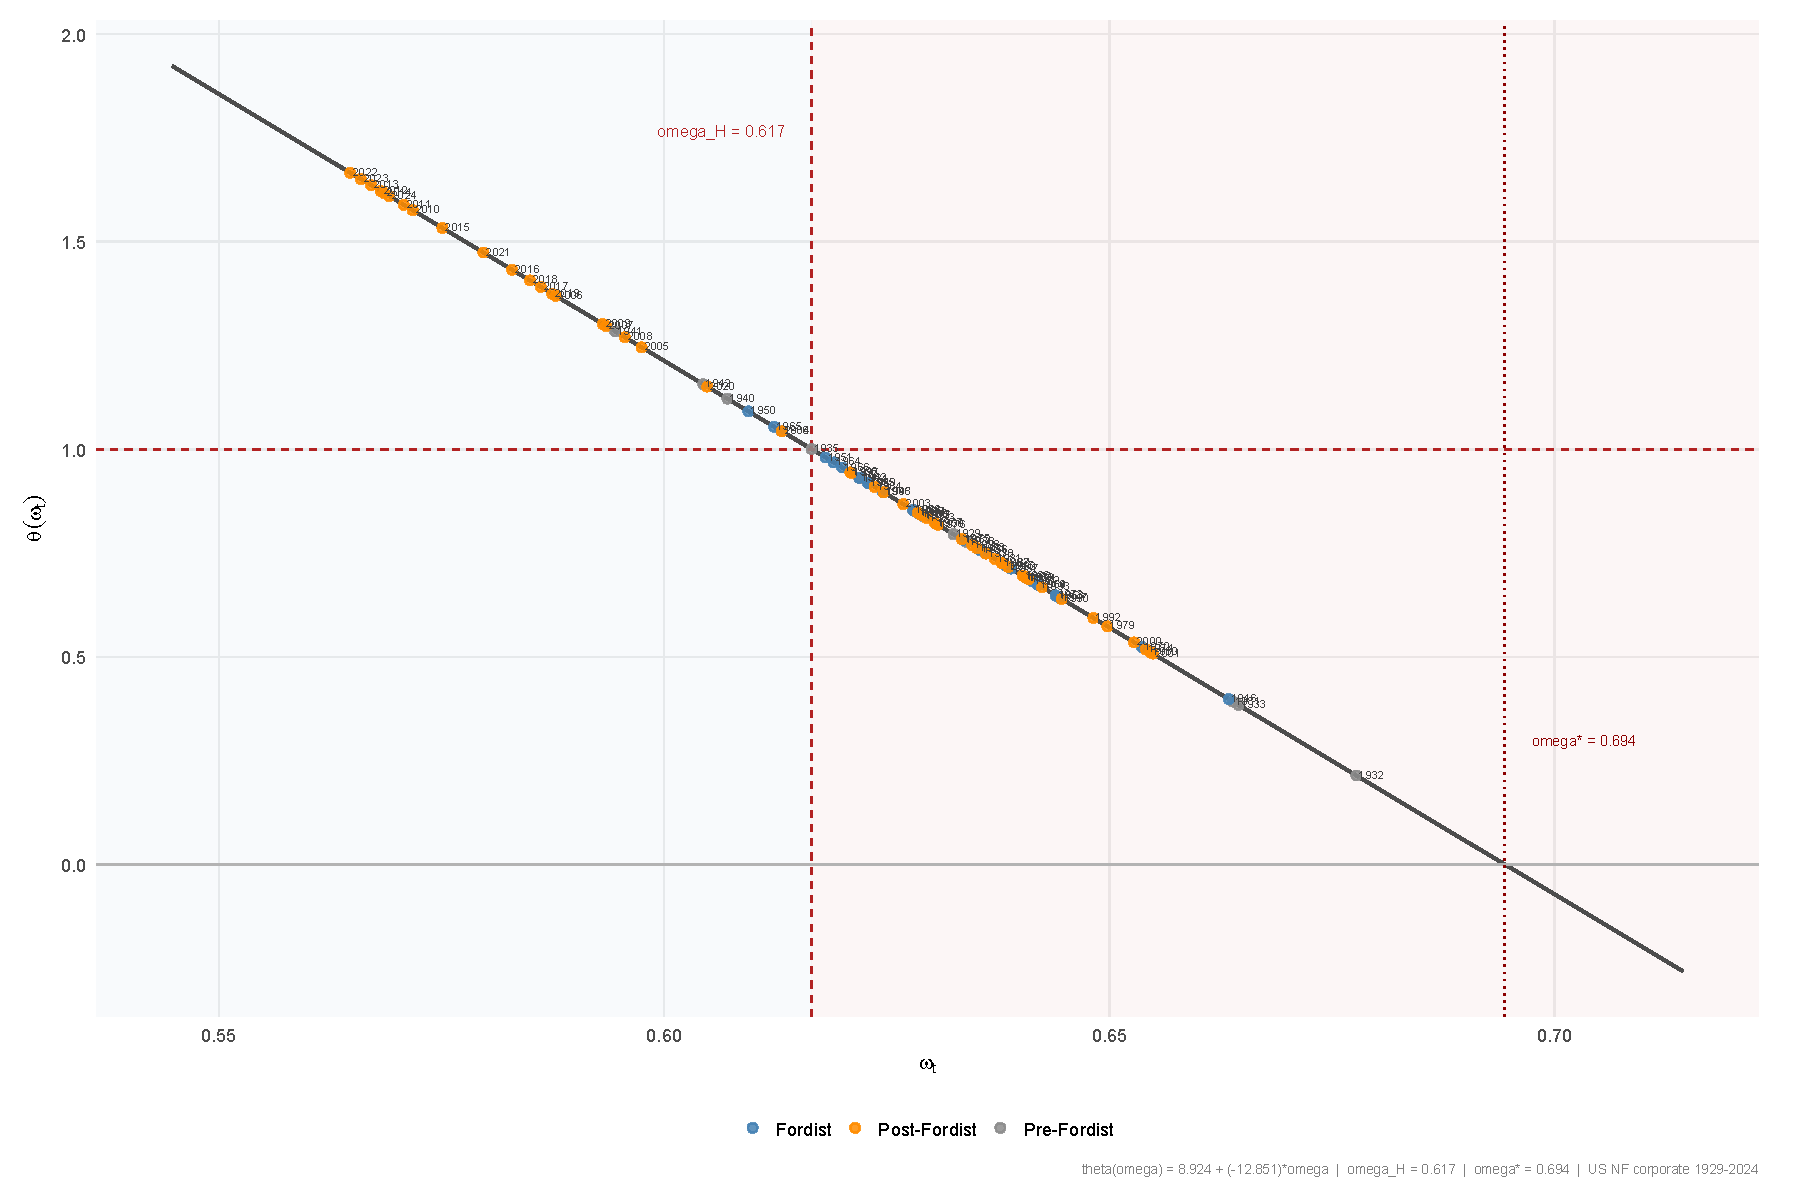
\includegraphics[scale=0.6]{figures/r1_theta_omega_scatter_full.pdf}
	\subcaption*{Dashed vertical lines mark
		the Harrodian knife-edge ($\omega_H = 0.617$) and the crisis boundary
		($\omega^* = 0.694$). Points colored by accumulation regime.}
\end{figure}

% ---- Error correction -------------------------------------------------------

The loading vector under $r = 1$ reveals the adjustment structure of the
system. Output does not error-correct to the MPF ($\hat{\alpha}_y = 0.011$,
$t = 0.74$), while capital ($t = 2.89$) and the wage share ($t = 3.11$)
adjust significantly (Table~\ref{tab:sa:alpha},
Appendix~\ref{app:sa:alpha}). This is the empirical counterpart of the
theoretical architecture developed in
Section~\ref{sec:analytical_framework}: the MPF is a supply-side locus
defining productive capacity, but output deviations from the frontier ---
capacity utilization --- are demand-determined. The frontier disciplines
accumulation and distribution, not output directly.

% ---- Capacity utilization ---------------------------------------------------

The structural capacity utilization rate $\hat{\mu}_t$ is constructed by
pinning the frontier at $\hat{\mu}(1948) = 0.80$ (Federal Reserve
benchmark) and accumulating forward and backward via the unbalanced growth
closure $g(Y^p_t) = \hat{\theta}(\omega_t) \cdot g(K_t)$.\footnote{Construction
	details and the ECT-based alternative $\hat{\mu}^{ect}_t$ are in
	Appendix~\ref{app:sa:mu_construction}.} Figure~\ref{fig:mu_us} displays
the resulting series.

\begin{figure}[H]
	\centering
	\caption{Capacity utilization $\hat{\mu}_t$, US Non-Financial
		Corporate Sector, 1929--2024. Dashed line at $\hat{\mu} = 1$ (full
		frontier utilization). Frontier pinned at $\hat{\mu}(1948) = 0.80$.
		Dotted vertical line marks the Fordist/Post-Fordist break (1973).}

	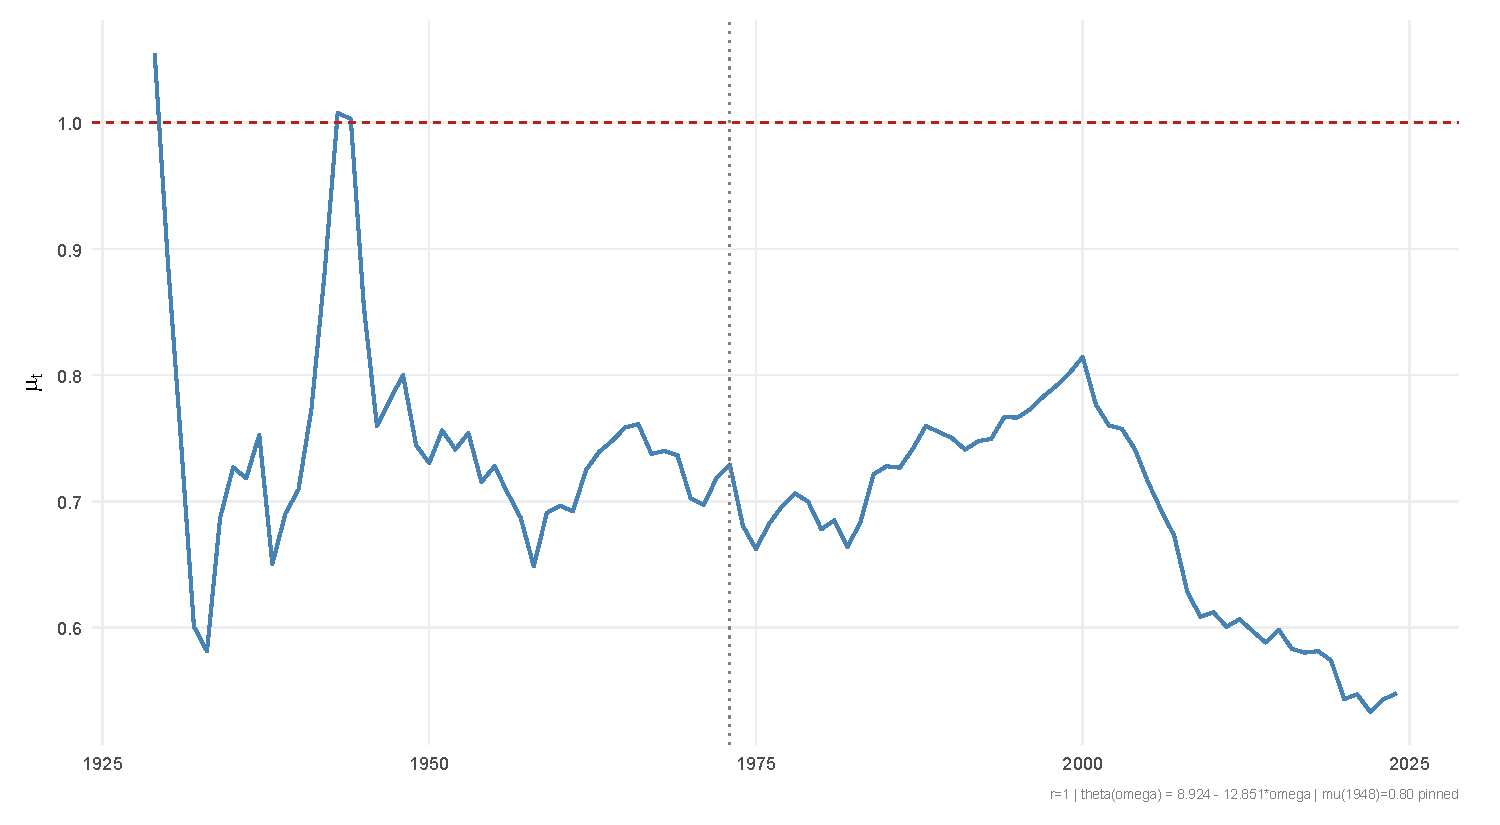
\includegraphics[width=\textwidth]{figures/r1_mu_capacity_utilization.pdf}
	\label{fig:mu_us}
\end{figure}

Three features of the $\hat{\mu}_t$ series carry structural significance
for interpreting the stagnation tendencies that Stages~B and~C map across
regimes.

First, the wartime years 1943--44 are the only observations at or above
the frontier ($\hat{\mu} \geq 1.0$), confirming that full capacity
utilization in the US non-financial corporate sector is historically
exceptional --- a wartime mobilization phenomenon, not a condition that
the Fordist settlement reproduced in peacetime. The Fordist sub-period
mean ($\bar{\hat{\mu}} \approx 0.73$) lies well below the frontier,
which means the over-accumulation stagnation tendency was structurally
operative throughout: capital accumulated, on average, faster than
productive capacity expanded. The Fordist institutional settlement did
not eliminate this tendency; it managed it --- primarily through Taylorist
compositional upgrading of the capital stock, which held real capital
productivity ($B_r$) on an ascending path even as the demand-utilization
gap persisted.

Second, the Fordist observations cluster near the knife-edge $\omega_H =
0.617$: the wage compromise that anchored the productivity-indexed wage
norm kept $\omega_t$ in a range where $\hat{\theta}$ oscillated between
sub- and super-Harrodian territory, making regime alternation empirically
operative. The over-accumulation stagnation tendency was present throughout
but was periodically counteracted by episodes of demand activation and
compositional upgrading --- the institutional mechanisms that Stage~B will
decompose at the swing level.

Third, the Post-Fordist era (1974--2024) exhibits a secular decline in
$\hat{\mu}$ from $0.74$ to $0.55$ (2024), driven by the regime shift to
$\bar{\theta} = 1.021$ --- sub-Harrodian on average. The productive
capacity frontier now grows \emph{faster} than the capital stock, and
the widening utilization gap reflects the structural mismatch between
the economy's capacity-generating potential and realized accumulation.
This is not a demand shortfall in the Keynesian sense but a
classical-Marxian structural condition: the productive frontier expands
faster than the conditions for its profitable utilization can be organized,
registering the exhaustion of the Fordist institutional settlement rather
than a cyclical demand failure.

Stage~A thus establishes the structural precondition for the analysis that
follows: $\hat{\theta} < 1$ at the sample mean means that the
over-accumulation stagnation tendency --- downward pressure on
profitability arising from capital accumulating faster than productive
capacity expands --- is structurally operative throughout the Fordist
period. What remains to be determined is which institutional channels
counteracted this tendency during the functional period (1951--1966), how
multiple tendencies converged into structural crisis in 1966--1970, and
through what behavioral mechanism the Fordist settlement reproduced
profitability for as long as it did. These are the questions that
Stages~B and~C respectively address.




% s26_us_draft_v2.tex
% §2.6 Stage B: Profitability Analysis — United States
% Second pass: WLM 3.1 + Jargon Calibration + hetpe-academic-writing
% Explanatory mode on — framework assumed established in §2.3
% Date: 2026-04-06



\subsubsection{Stage B: Profitability Analysis --- United States}
\label{sssec:stageB_us}

% ---- P1: Contribution statement up front ------------------------------------

The four-channel decomposition developed in this stage extends the
standard \citet{Weisskopf1979} framework by separating nominal capital
productivity into its relative-price and real components:
%
\begin{equation}
	r_t = \hat{\mu}_t \cdot \frac{P_Y}{P_K}\bigg|_t \cdot B_{r,t} \cdot \pi_t
	\label{eq:4ch_identity}
\end{equation}
%
or in log-additive growth form:
%
\begin{equation}
	\Delta\ln r_t = \underbrace{\Delta\ln\hat{\mu}_t}_{\phi_\mu}
	+ \underbrace{\Delta\ln(P_Y/P_K)_t}_{\phi_{p}}
	+ \underbrace{\Delta\ln B_{r,t}}_{\phi_{B}}
	+ \underbrace{\Delta\ln\pi_t}_{\phi_\pi}
	\label{eq:4ch_log}
\end{equation}
%
The analytical contribution of this disaggregation is not arithmetical
precision for its own sake. In the three-channel nominal framework, a
world-market price shock that raises the cost of capital goods relative
to output prices is absorbed entirely into the technology channel and
interpreted as a deterioration of productive efficiency. The four-channel
identity separates price-mediated from quantity-mediated capital
productivity dynamics, making it possible to distinguish a structural
technology failure from a geopolitical price shock --- a distinction that
the 1972--1974 episode, examined below, makes empirically consequential.

% -----------------------------------------------------------------------
% Table B3 — place before Paragraph 2 (sub-period means)
% -----------------------------------------------------------------------

% tab_B3_subperiod.tex
% Weisskopf components: sub-period means
% Standalone fragment: \input{tables/tab_B3_subperiod}

\begin{table}[htbp]
\centering
\caption{Weisskopf components: sub-period means,
  US Non-Financial Corporate Sector, 1940--2024.}
\label{tab:B3_subperiod}
\small
\begin{threeparttable}
\begin{tabular}{%
  l
  l
  S[table-format=1.3]
  S[table-format=1.3]
  S[table-format=1.3]
  S[table-format=1.3]
  S[table-format=1.3]
}
\toprule
{Period} & {Years}
  & {$\bar{r}$}
  & {$\bar{\mu}$}
  & {$\overline{Py/PK}$}
  & {$\bar{B}_{r}$}
  & {$\bar{\pi}$} \\
\midrule
Pre-Fordist/WWII   & 1940--1944 & 0.214 & 0.875 & 1.369 & 0.457 & 0.389 \\
\midrule
Early Fordist      & 1945--1966 & 0.187 & 0.737 & 1.176 & 0.586 & 0.369 \\
Late Fordist       & 1967--1973 & 0.189 & 0.723 & 1.140 & 0.635 & 0.360 \\
\midrule
Post-Fordist onset & 1974--1978 & 0.169 & 0.686 & 1.025 & 0.664 & 0.363 \\
\addlinespace[2pt]
Post-Fordist full$^{\dagger}$
                   & 1974--2024 & 0.183 & 0.681 & 1.041 & 0.683 & 0.385 \\
\bottomrule
\end{tabular}
\begin{tablenotes}
\small
\item \textit{Notes:}
  $r = \text{GOS}/\text{KNC}$ (nominal);
  $\hat{\mu}$ from Stage~A MPF (pinned at $\hat{\mu}_{1948}=0.80$);
  $B_{r} = \text{GVA}_{r}/(\text{KNR}\cdot\hat{\mu})$;
  $Py/PK$ = GDP deflator / capital price deflator;
  $\pi = \text{GOS}/\text{GVA}$.
  Primary estimation window: 1945--1978.
\item[$\dagger$] Reported for context; outside the primary estimation window.
\end{tablenotes}
\end{threeparttable}
\end{table}


The sub-period means in Table~\ref{tab:B3_subperiod} register the
macroscopic signature of a functional accumulation regime. The nominal
profit rate held within a narrow band (0.187--0.189) across the Early and
Late Fordist sub-periods even as mean capacity utilization fell
monotonically from 0.737 in the Early Fordist to 0.723 in the Late Fordist
and 0.686 at the Post-Fordist onset --- a progressive deterioration in the
activation of productive capacities that Stage~A attributed to the
structural over-accumulation stagnation tendency identified in the previous
stage. The profit share compressed modestly from 37\% to 36\%, consistent
with the distributional pressure imposed by full-employment commitment.
The offsetting channel was real capital productivity at normal capacity,
rising from 58.6\% to 63.5\% across the Fordist transition ---
Taylorist compositional upgrading performing the compensatory work that
demand and distribution could no longer sustain
(Figures~\ref{fig:B1b} and~\ref{fig:B1c}).

The four-channel decomposition makes visible a structural headwind that
the three-channel framework suppresses: the output-to-capital relative
price compressed monotonically throughout --- mean $P_Y/P_K$ falling from
1.369 to 1.176 to 1.140 to 1.025, a decline of 25 percentage points
across the full window. Real capital productivity therefore had to rise
not merely to offset the falling activation of productive capacity but
to do so against a secular relative-price deterioration that a
three-channel decomposition would attribute entirely to the technology
channel without distinguishing price from quantity sources of capital
productivity dynamics.

% -----------------------------------------------------------------------
% Table B2 — place before Paragraph 3 (turning-point structure)
% -----------------------------------------------------------------------

% tab_B2_peaktotrough.tex
% Four-channel decomposition of profit-rate swings
% Standalone fragment: \input{tables/tab_B2_peaktotrough}

\begin{table}[htbp]
\centering
\caption{Four-channel decomposition of profit-rate swings,
  US Non-Financial Corporate Sector, 1951--1974.}
\label{tab:B2_peaktotrough}
\small
\begin{adjustbox}{max width=\textwidth}
\begin{threeparttable}
\begin{tabular}{%
  l
  l
  S[table-format=-1.3]
  S[table-format= 1.3]
  S[table-format=-1.3]
  S[table-format=-1.3]
  S[table-format= 1.3]
  S[table-format= 1.3]
  l
}
\toprule
{Period} & {Type}
  & {$\Delta\ln r$}
  & {$s_{\mu}$}
  & {$s_{Py/PK}$}
  & {$s_{B_{r}}$}
  & {$s_{\pi}$}
  & {$\Sigma$}
  & {Dominant} \\
\midrule
1951--1954 & Contraction
  & -0.133 & 0.417 &  0.041
  &  0.057 & 0.485 & 1.000 & $\pi$ \\
\addlinespace[3pt]
1954--1955 & Expansion
  & +0.100 & 0.172 & $\mathit{-0.472}^{\dagger}$
  &  0.777 & 0.523 & 1.000 & $B_{r}$ \\
\addlinespace[3pt]
1955--1958 & Contraction
  & -0.191 & 0.602 &  0.054
  &  0.091 & 0.253 & 1.000 & $\mu$ \\
\addlinespace[3pt]
1958--1966 & Expansion
  & +0.336 & 0.477 &  0.132
  &  0.224 & 0.167 & 1.000 & $\mu$ \\
\addlinespace[3pt]
1966--1970 & Contraction
  & -0.269 & 0.298 &  0.065
  &  0.292 & 0.345 & 1.000 & $\pi$, $\mu$, $B_{r}$ \\
\addlinespace[3pt]
1970--1972 & Expansion
  & +0.066 & 0.341 & $\mathit{-0.104}^{\dagger}$
  &  0.235 & 0.527 & 1.000 & $\pi$ \\
\addlinespace[3pt]
1972--1974 & Contraction
  & -0.164 & 0.331 &  0.578
  & $\mathit{-0.130}^{\dagger}$ & 0.221 & 1.000 & $Py/PK$ \\
\bottomrule
\end{tabular}
\begin{tablenotes}
\small
\item \textit{Notes:}
  $\Delta\ln r = \phi^{\mu} + \phi^{Py/PK} + \phi^{B_{r}} + \phi^{\pi}$
  (exact); $s_{j}$ sum to unity.
  $r = \text{GOS}/\text{KNC}$;
  $B_{r} = \text{GVA}_{r}/(\text{KNR}\cdot\hat{\mu})$;
  $Py/PK$ = GDP deflator / capital deflator;
  $\hat{\mu}$ from Stage~A MPF.
\item[$\dagger$] Offsetting channel: contribution moves against the swing direction.
\end{tablenotes}
\end{threeparttable}
\end{adjustbox}
\end{table}


\begin{figure}[htbp]
	\centering
	\caption{Offsetting trajectories of the Fordist compensation mechanism,
	US Non-Financial Corporate Sector, 1940--1978.}
	\begin{subfigure}[t]{0.48\textwidth}
		\centering
		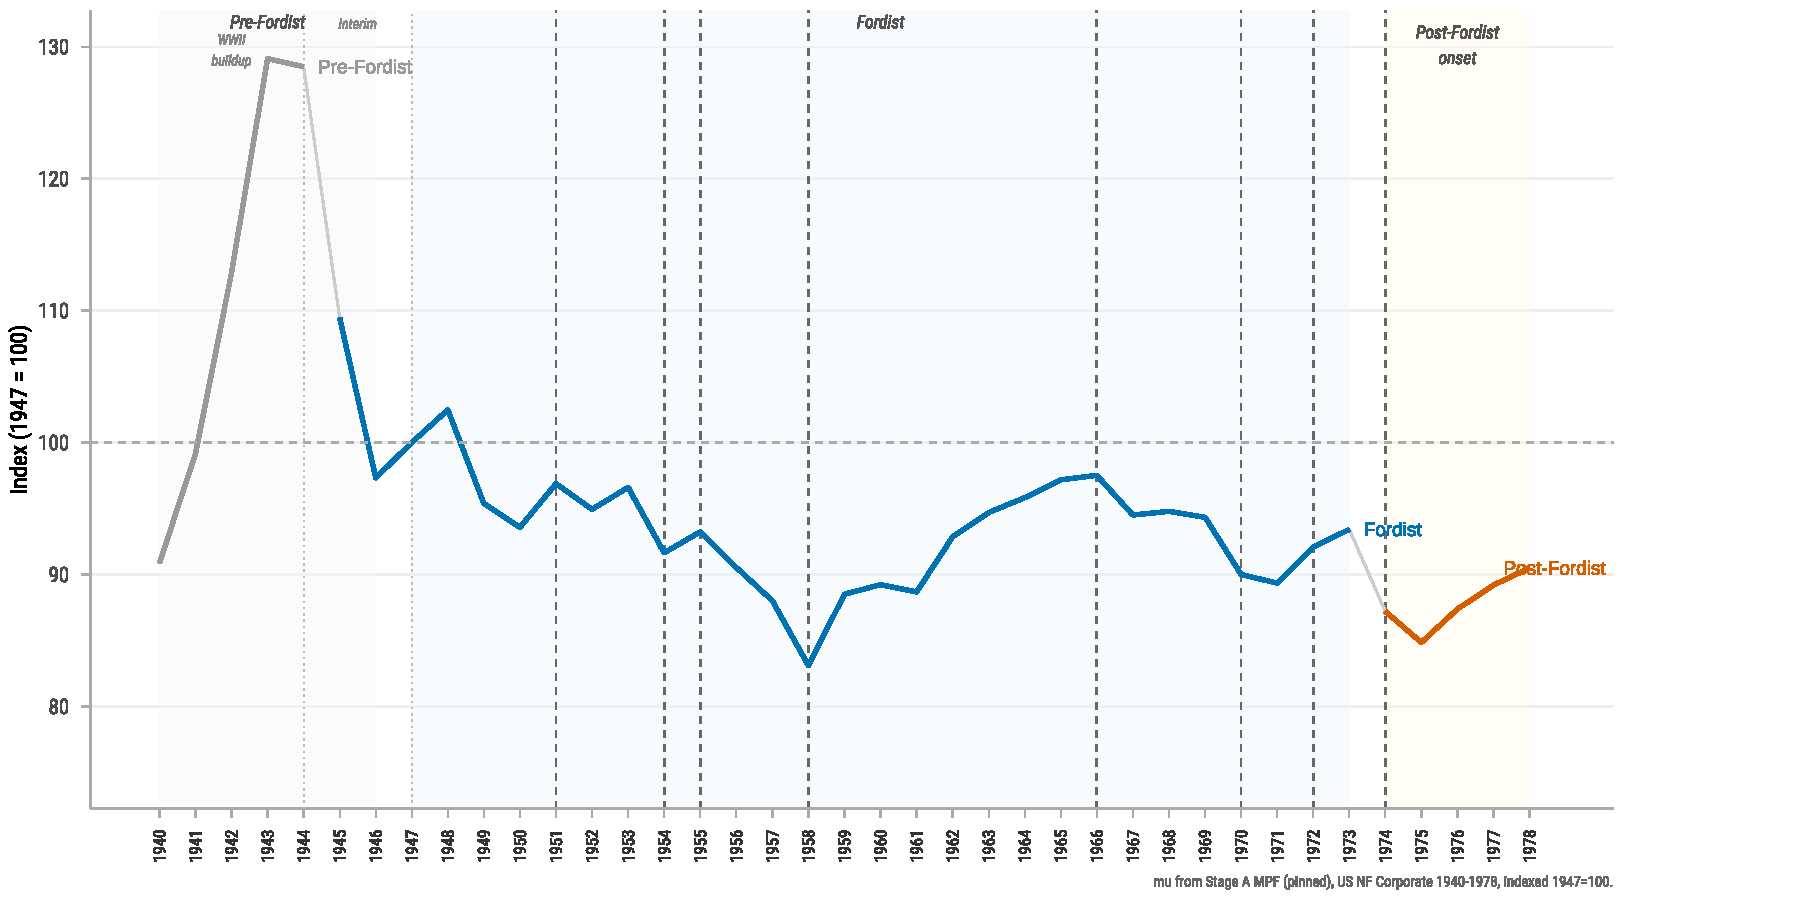
\includegraphics[width=\textwidth]{figures/fig_B1b_mu_levels}
		\caption{Capacity utilization $\hat{\mu}_{t}$,
			indexed 1947\,=\,100.}
		\label{fig:B1b}
	\end{subfigure}
	\hfill
	\begin{subfigure}[t]{0.48\textwidth}
		\centering
		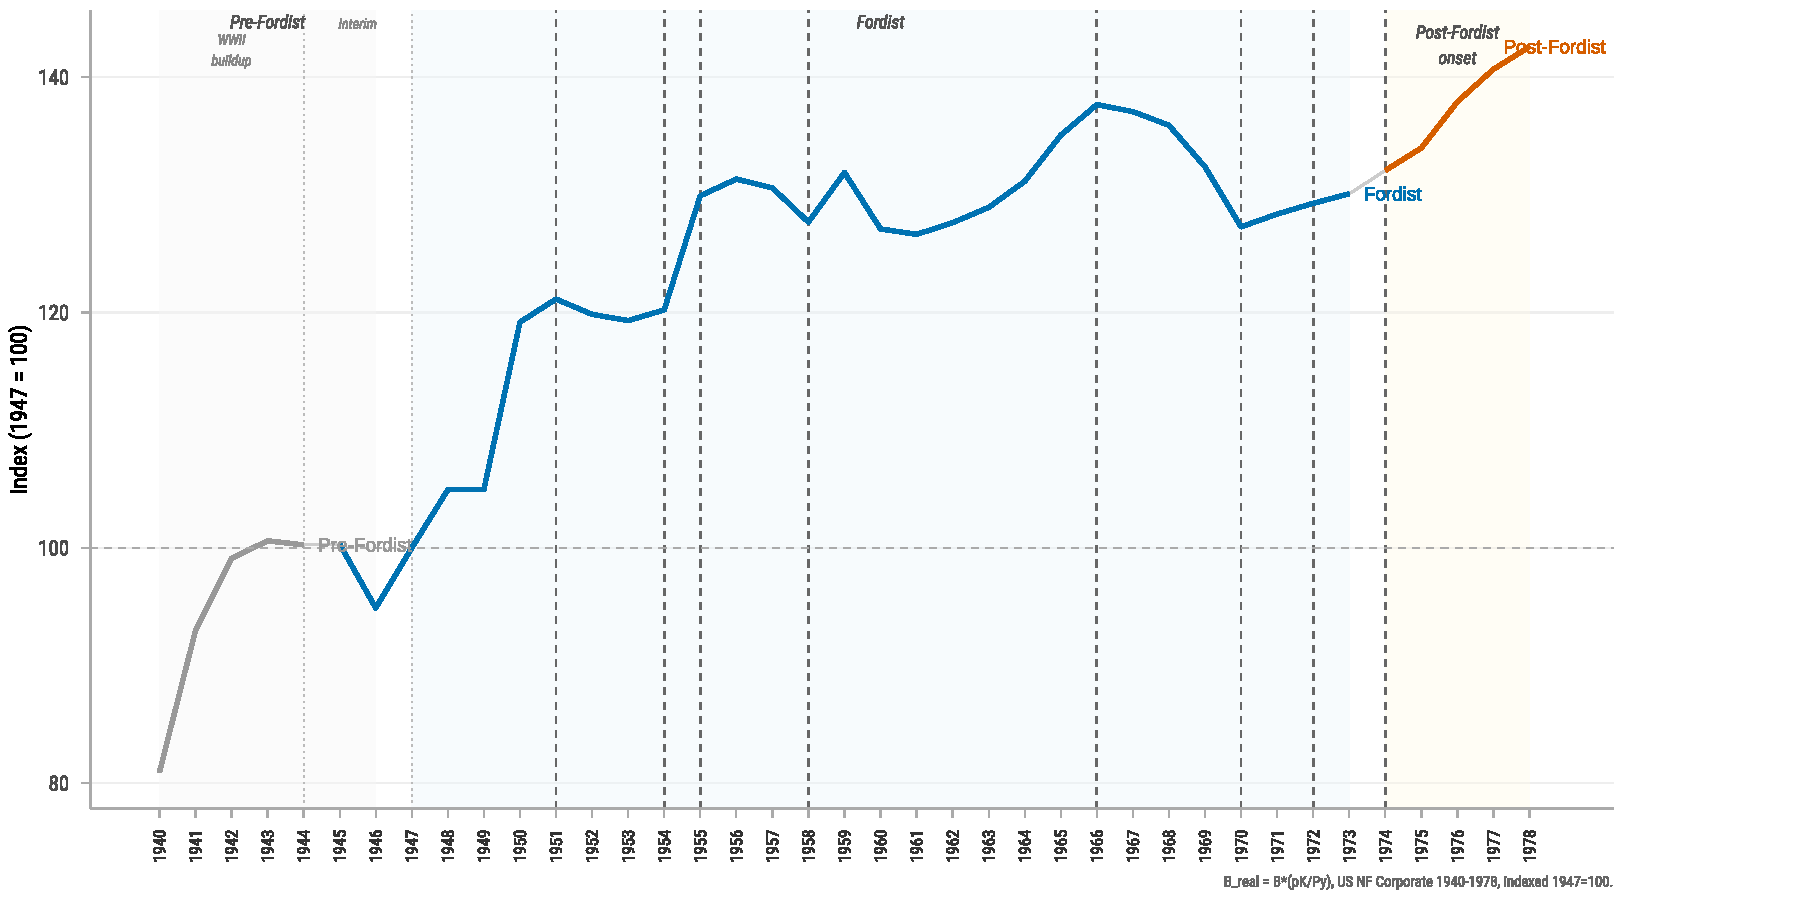
\includegraphics[width=\textwidth]{figures/fig_B1c_Breal_levels}
		\caption{Real capital productivity $B_{r,t}$,
			indexed 1947\,=\,100.}
		\label{fig:B1c}
	\end{subfigure}
	\label{fig:B1bc}
\end{figure}

Figure~\ref{fig:B4} identifies seven turning points on $r_t$ between
1951 and 1974, organized into the swing-level episodes whose channel
composition Table~\ref{tab:B2_peaktotrough} decomposes. Turning points
are identified on the profit rate rather than on output or employment
because a profit-rate contraction can begin while output is still
expanding --- precisely the structural condition that the over-accumulation
stagnation tendency generates: capital accumulates, productive capacity
expands, but the utilization of that capacity in profitable production
declines. The seven swings identified span two qualitatively distinct
phases: the first four (1951--1966) constitute the Fordist settlement's
normal cycle, cumulatively lifting $r_t$ to its 1966 peak; the remaining
three (1966--1974) constitute its structural dissolution under the
convergence of stagnation tendencies that institutional containment could
no longer separately counteract.

% -----------------------------------------------------------------------
% Figure B4 — place after Paragraph 3 (turning-point structure)
% -----------------------------------------------------------------------

\begin{figure}[htbp]
	\caption{Profit rate with identified turning points,
		US Non-Financial Corporate Sector, 1940--1978.}
	\label{fig:B4}
	\centering
	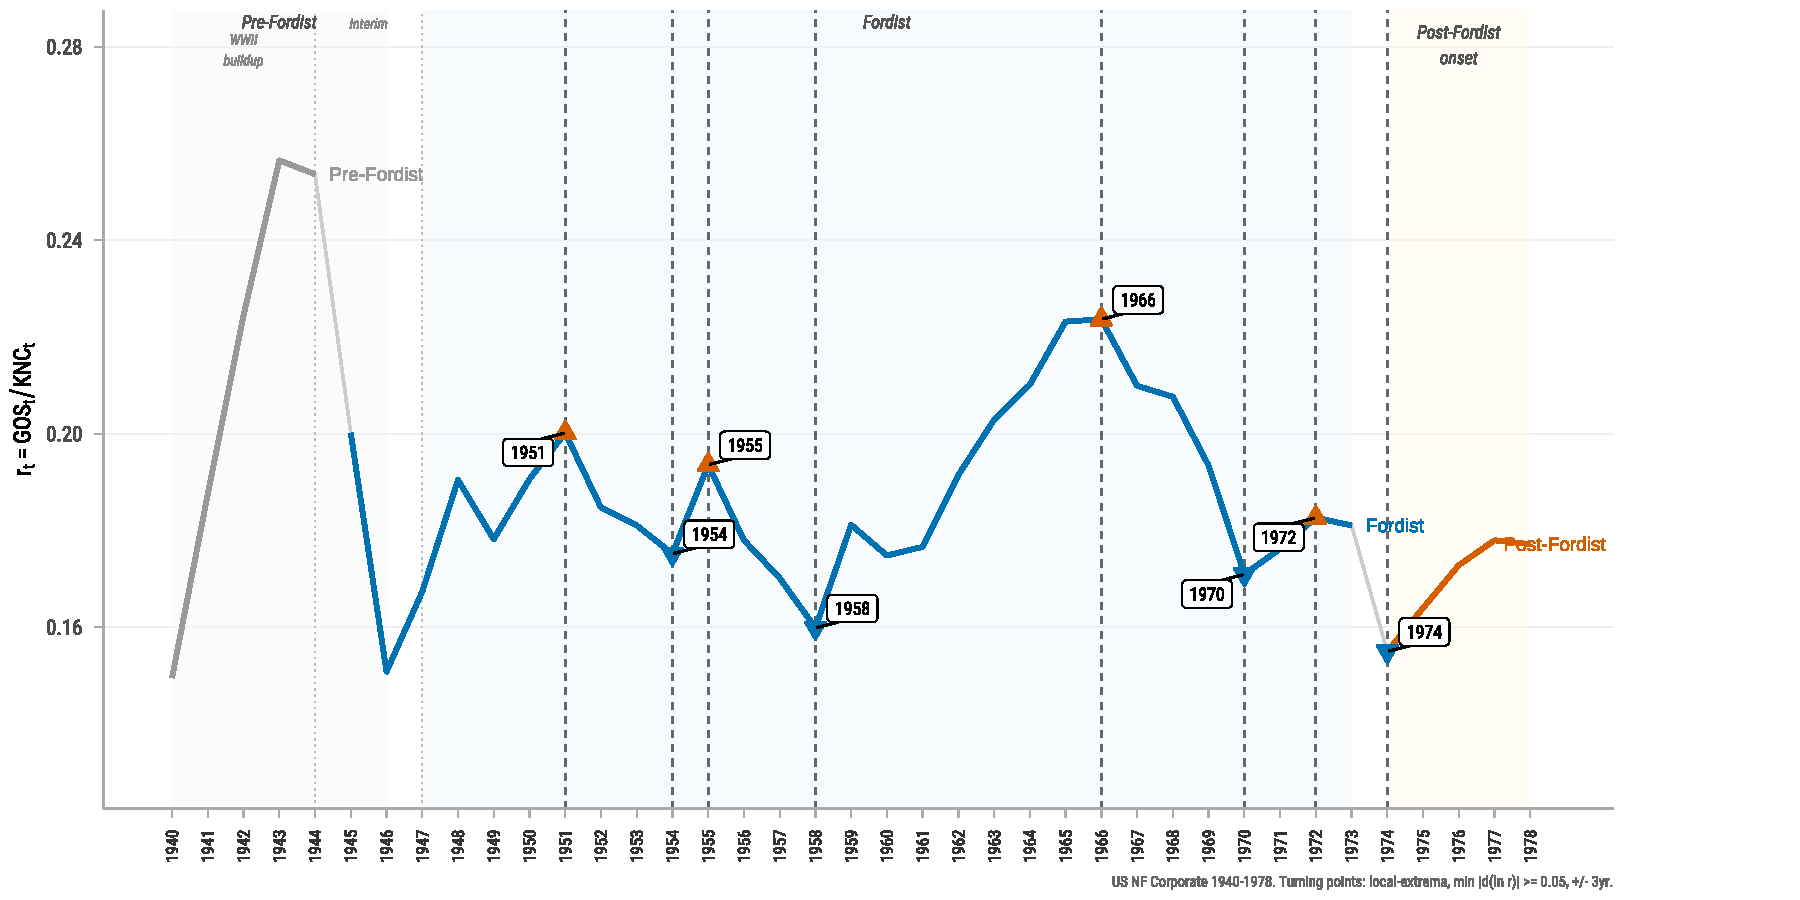
\includegraphics[width=\textwidth]{figures/fig_B4_profit_rate_turning_points}
\end{figure}

The 1951--1954 and 1955--1958 contractions are the diagnostic signature
of a relatively functional accumulation regime --- one in which the
institutional settlement is absorbing stagnation tendencies because only
one structural channel is under serious pressure at a time. During the
1951--1954 contraction ($\Delta r = -13.3\%$), the distributional channel
accounts for 48.5\% of the decline while the demand channel contributes
41.7\%, placing this episode in the category of a distributional
compression of surplus value --- the profit-squeeze configuration in which
rising labor-market strength erodes the profit share before the demand
channel fully adjusts \citep{Basu2019}. The 1955--1958 contraction
($\Delta r = -19.1\%$) presents the opposite configuration: the demand
channel accounts for 60.2\% of the decline, with the profit share
contributing a secondary role. The distributional stagnation tendency was
contained; it was the realization of demand conditions --- the capacity
of productive activity to find profitable outlets --- that drove the
contraction \citep{Okishio2022}. Both episodes are structurally consistent
with a functional regime: single-channel dominance between 48 and 60\%
signals that partial reconfiguration --- demand stimulus for a demand-led
contraction, distributional adjustment for a profit-led one --- was
structurally sufficient without requiring major institutional transformation.

The recovery between these two contractions --- the 1954--1955 expansion
--- was technology-led, with $B_r$ accounting for 77.7\% of the rebound
while the relative-price channel offset at $-47.2\%$, confirming that
Taylorist compositional upgrading was already performing compensatory work
within the normal Fordist cycle. The 1958--1966 expansion
($\Delta r = +33.6\%$) registers the opposite condition: all four channels
contributing positively without any offsetting tendency placing downward
pressure on profitability. Military-Keynesian fiscal expansion --- the
demand management apparatus that the Fordist settlement had institutionalized
--- raised capacity utilization sufficiently to account for 47.7\% of the
profit rate recovery \citep{Baker1996}. Demand activation coupled with
rising real capital productivity (22.4\%), which the high-utilization
environment induced through the absorption of higher-vintage productive
capacity. The still-favourable $P_Y/P_K$ environment amplified the demand
effect (13.2\%), while the distributional channel contributed the least
(16.7\%), consistent with the productivity-indexed wage compromise the
Fordist institutional settlement had routinized. The 1958--1966 period is
the accumulation regime at its most coherent: institutional mechanisms
aligned, all channels reinforcing, stagnation tendencies present but
counteracted --- and in counteracting them, building the structural
preconditions of their eventual convergence.

The 1966--1970 contraction ($\Delta r = -26.9\%$) is where the analytical
value of the stagnation tendencies framework becomes fully operative.
What the decomposition records is not merely a large decline but the
configuration in which multiple stagnation tendencies ceased to be
contained simultaneously, converging into structural crisis. No single
channel dominates: the profit share accounts for 34.5\% of the compounded
decline, real capital productivity for 29.2\%, and the demand channel
for 29.8\%, with the relative-price channel contributing an additional
6.5\%. All channels drag simultaneously; no offsetting force is operative.
The contrast with the earlier contractions is constitutive of the
empirical finding: those episodes registered single-channel dominance
precisely because the Fordist institutional settlement was containing
distributional conflict through productivity-indexed wages, sustaining
demand through fiscal management, and holding Taylorist production
organization sufficiently stable to generate real labor productivity growth
at a higher pace than induced mechanization net of relative prices. By
1966, that multi-channel containment capacity was exhausted.

Three stagnation tendencies converged. Full-employment conditions sustained
through military expenditures tightened the labor market, enhancing
working-class bargaining power and directly eroding the profit share ---
the distributional stagnation tendency, previously contained by the
productivity-indexed wage norm, broke its institutional ceiling
\citep{Baker1996, Vidal2019}. The Taylorist work organization that had
anchored $B_r$ growth reached its productive limits: the systematic
separation of conception from execution that secured managerial control
over the labor process had simultaneously eroded the cooperative and
cognitive capacities on which further productivity improvement depended
--- the same deskilling that served accumulation became a fetter on its
continuation \citep{Braverman1998, Vidal2022}. The demand channel weakened
as the military-Keynesian stimulus reached its inflationary ceiling and
fiscal space for further expansion contracted. The near-equal weight of
these three mechanisms --- each accounting for between 29 and 35\% of the
profit-rate contraction --- is the empirical expression of institutional
containment failure: not a single-tendency crisis resolvable by partial
reconfiguration, but a structural crisis requiring wholesale regime
transformation \citep{Vidal2013, Vidal2019}.

The 1970--1972 period records a modest expansion ($\Delta r = +6.6\%$),
the smallest positive swing in the period of analysis: the profit share
led at 52.7\% as labor-market pressure eased temporarily, but the
relative-price channel offset at $-10.4\%$ --- the secular compression
of $P_Y/P_K$ was already working against profitability restoration even
during a period of distributional adjustment.

The 1972--1974 contraction ($\Delta r = -16.4\%$) delivers the most
analytically consequential result of the four-channel decomposition. In
the three-channel nominal framework, this contraction appears
technology-led: the capital productivity channel in nominal terms accounts
for the dominant share of the decline, historically interpreted as a
structural deterioration in the productive efficiency of the US capital
stock during the early 1970s. The four-channel decomposition disaggregates
that finding and records a qualitatively different interpretation. The
relative-price channel accounts for 57.8\% of the compounded decline;
real capital productivity, by contrast, offset $-13.0\%$ of the decline
--- real productive efficiency continued to improve despite the oil price
shock. Profitability fell in nominal terms not because productive capacity
stagnated but because the price of capital goods rose relative to the
price of output, reducing the nominal rate of return even as the real
productive frontier continued to expand. The world-market stagnation
tendency --- geopolitical price shock operating through $P_Y/P_K$ --- was
the mechanism, not a demand collapse or a structural technology failure.
This is the contribution that the four-channel identity makes visible:
the oil shock was a price-mediated transmission of an external stagnation
tendency into the domestic profit rate, acting through the relative-price
channel on a system whose institutional containment capacity had already
been exhausted in 1966--1970.

Figure~\ref{fig:B3} captures this structural progression through the
decomposition of channel shares across all seven profit-rate swings. What
the figure establishes is not merely a historical narrative of Fordist
profitability but a structural logic: the compensation mechanism through
which the Fordist accumulation regime reproduced profitability --- $B_r$
rising from 58.6 to 63.5 against simultaneous declines in capacity
utilization (from 0.875 to 0.72) and a secular compression of $P_Y/P_K$
(from 1.37 to 1.14) --- contained within it the conditions that brought
reproduction to a close. The mechanism was constitutive of the
over-accumulation regime: with the transformation elasticity near but
below unity ($\hat{\theta} = 0.918$ at the sample mean), each wave of
capital accumulation expanded productive capacity less than proportionally
to the stock it added. The Taylorist organization of production positioned
the mechanization frontier sufficiently high that new investment
systematically outperformed the capital it replaced, so that compositional
upgrading of the stock sustained $B_r$ growth in real terms even as the
marginal capacity return on accumulation declined. But that compensatory
mechanism carried a structural limit. The demand management that sustained
$B_r$ through high utilization and the absorption of high-vintage
productive capacity simultaneously generated full-employment conditions
that tightened the labor market, enhanced working-class bargaining power,
and placed downward pressure on the profit share through the distributional
stagnation tendency \citep{Baker1996, Vidal2019}. When Taylorist work
organization exhausted its productivity gains, the deskilling that had
secured managerial control eroded the cooperative conditions on which
further mechanization-induced productivity growth depended
\citep{Braverman1998, Vidal2022}. The drag imposed by the structural
over-accumulation tendency ($\hat{\theta} < 1$), previously dominated by
compositional upgrading, began to govern average dynamics. The mechanism
could not be sustained because the institutional conditions for its
operation were simultaneously the conditions for its own dissolution. 

% -----------------------------------------------------------------------
% Figure B3 — place after synthesis paragraph
% -----------------------------------------------------------------------

\begin{figure}[htbp]
	\caption{Channel composition of profit-rate swings,
		US Non-Financial Corporate Sector, 1951--1974.}
	\label{fig:B3}
	\centering
	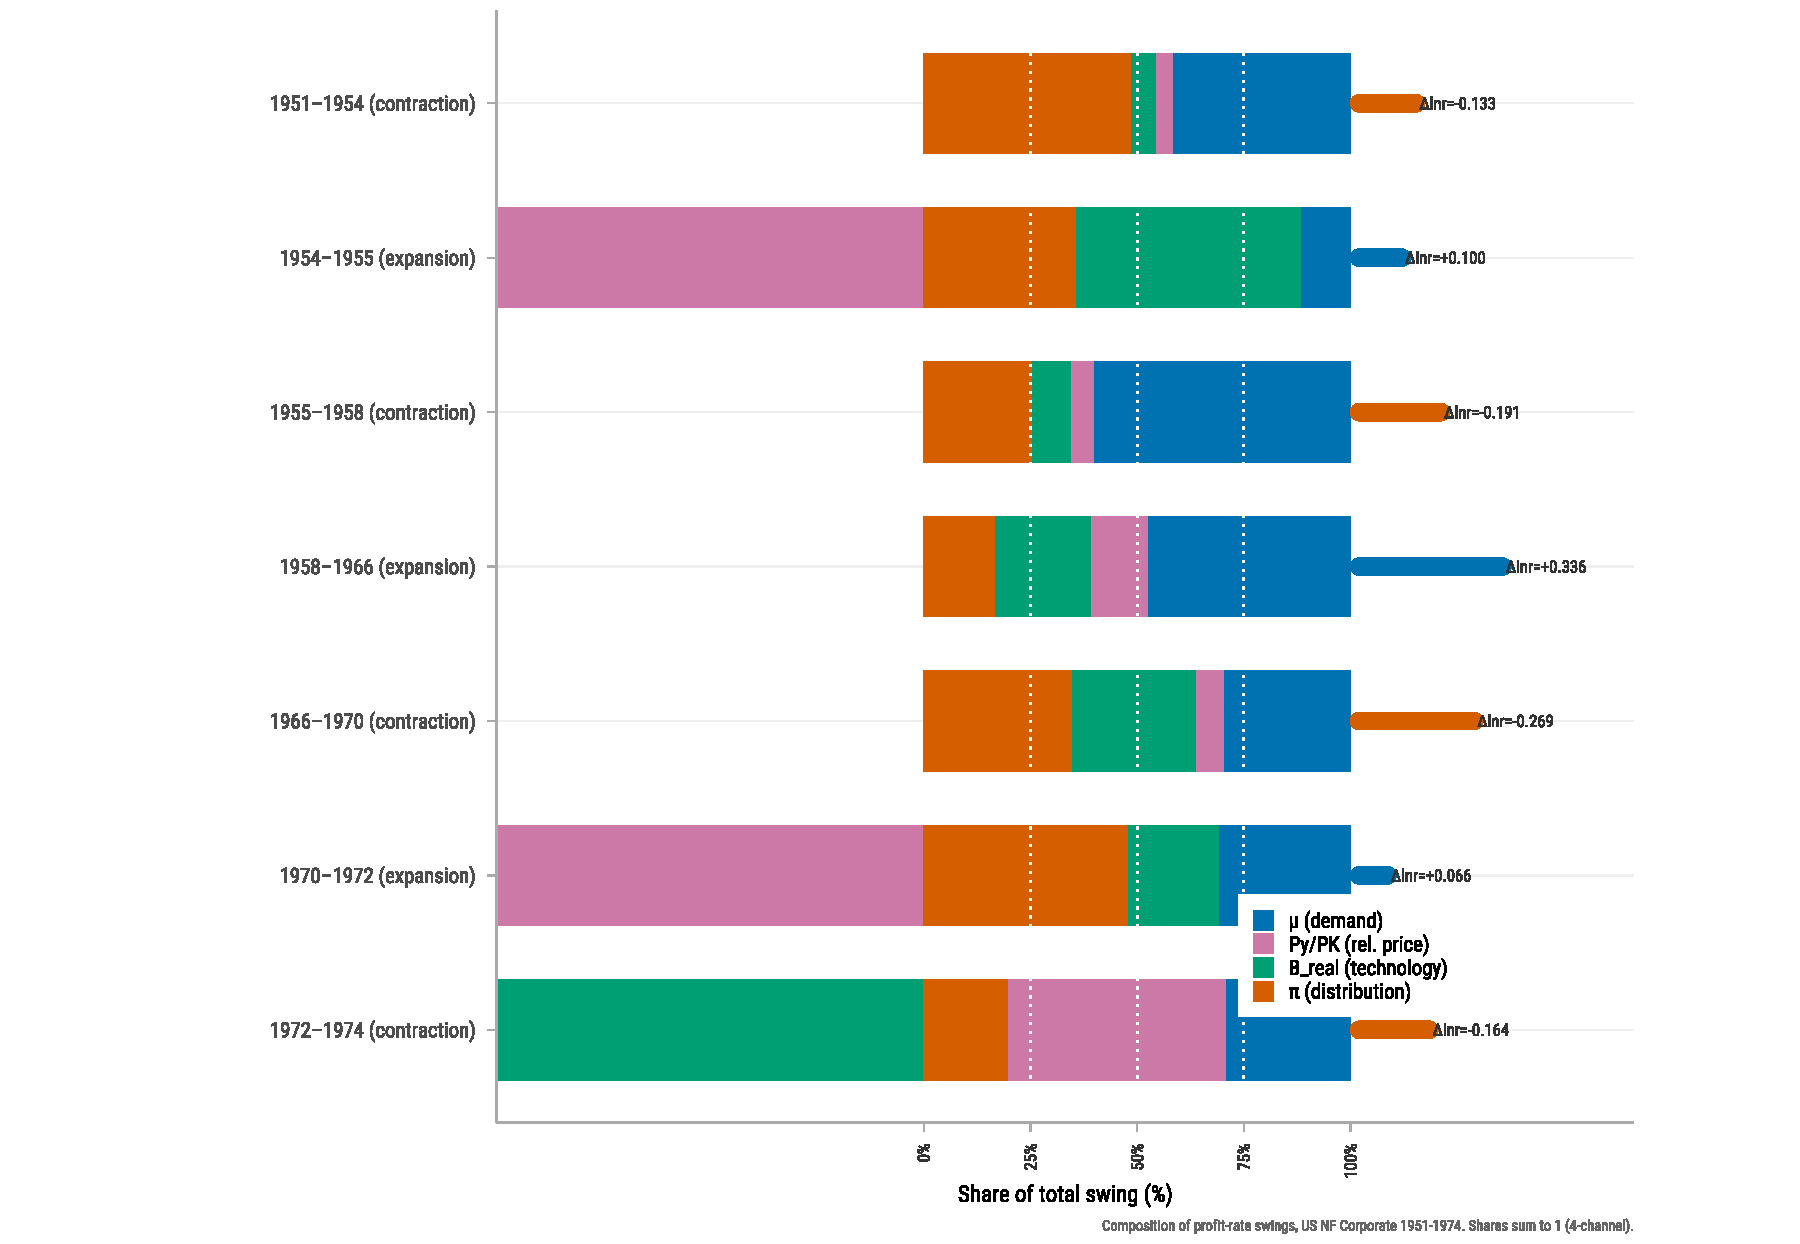
\includegraphics[width=\textwidth]{figures/fig_B3_swing_composition}
\end{figure}

The profitability decomposition has done what accounting can do:
separated the channels, identified their magnitudes, and distinguished
the structural crisis of institutional exhaustion from the world-market
price event that followed it. What it cannot reach --- not because of
a data limitation, but because it is an accounting identity --- is the
causal direction: whether demand activation was the mechanism that
counteracted over-accumulation, or whether over-accumulation was the
structural condition that made demand activation necessary in the first
place. That question is the object of Chapter~3.



\subsection{Chile}
\label{sec:results_chile}

\subsubsection{Stage A: The Mechanization Possibility Frontier under a
Balance-of-Payments Constraint}
\label{sec:results_cl:stage_a}

The Chilean mechanization possibility frontier is BoP-constrained: each
unit of machinery accumulation raises the structural import requirement
by $\hat{\zeta}_1 = 0.930$, so the productive frontier is not identified
independently of the external balance. The identification internalizes
this constraint through a recursive two-stage structure. Stage~1
recovers the structural import propensity as a cointegrating relation in
the state vector $(m_t,\,k_t^{ME},\,nrs_t,\,\omega_t)'$, split at 1973
to accommodate the coup-period structural break; the resulting
error-correction term $ECT_{m,t}$ enters Stage~2 as the threshold
indicator for a CLS-TVECM that estimates the productive frontier with
the external balance constraint as an endogenous shadow price on
mechanization.

% ---- Stage 1: Import propensity ----------------------------------------

\paragraph{Stage 1 --- Structural import propensity.}

Both sub-samples confirm $r = 1$. Pre-1973, the trace statistic of $54.44$
exceeds the 5\% critical value of $53.12$; post-1973, the trace of $70.75$
decisively exceeds the 1\% critical value of $60.16$. The $m$-normalized pre-1973
cointegrating vector is:
%
\begin{equation}
    m_t \;=\; -5.804 \;+\; 0.930\,k_t^{ME}
              \;+\; 0.445\,nrs_t
              \;-\; 3.919\,\omega_t
              \;+\; ECT_{m,t}
    \label{eq:cl:import_cv}
\end{equation}

Three structural channels organize the long-run import propensity. Each
unit increment in the imported machinery stock raises structural import
demand by $\hat{\zeta}_1 = 0.930$, tracing the mechanism identified by
\citet{Kaldor1959} whereby capital-goods imports constitute a necessary
input to productive capacity expansion under peripheral industrialization
rather than a discretionary or cyclically adjustable outlay. The
diversion of non-reinvested profits into consumption-goods imports
contributes $\hat{\zeta}_2 = 0.445$ --- a surplus-drain effect through
which the consumption-import propensity of the non-wage income circuit
generates a persistent structural claim on foreign exchange
\citep{Palma1989}. A unit increase in the wage share compresses
structural import demand by $|\hat{\zeta}_3| = 3.919$ --- the strongest
channel by standardized impact ($0.269$) --- reflecting the structurally
lower import content of the wage-goods basket relative to the non-wage
circuit.

The loading structure identifies which variables error-correct to the
long-run import relation. Import demand ($\hat{\alpha}_m = -0.178$,
$p = 0.011$) and the wage share ($\hat{\alpha}_\omega = -0.066$,
$p = 0.018$) are not weakly exogenous: both respond to deviations from
the long-run propensity. The imported machinery stock and non-reinvested
surplus are weakly exogenous: they drive the system toward its long-run
propensity without themselves adjusting to departures from it. Capital
goods accumulation and surplus distribution are therefore forcing
variables of the external balance, not equilibrating ones.

Post-1973, the structural configuration shifts sharply. The
machinery-accumulation coefficient falls to $\hat{\zeta}_1 = 0.309$
--- a two-thirds reduction in the long-run import requirement per unit
of mechanization, registering the collapse of machinery investment
under post-coup shock therapy. The wage-share compression channel
intensifies to $|\hat{\zeta}_3| = 7.128$, marking the distributional
violence of post-coup wage suppression as a structural determinant of
import compression rather than a merely cyclical one.

% ---- Stage 2: Productive frontier --------------------------------------

\paragraph{Stage 2 --- Productive frontier and BoP shadow price.}

The Stage~2 CLS-TVECM estimates the productive frontier on the state
vector $(y_t,\,k_t^{NR},\,k_t^{ME},\,\omega_t k_t^{ME})'$ with
$\hat{\gamma} = -0.1394$ as the estimated threshold on $ECT_{m,t-1}$.
The $y$-normalized frontier cointegrating vector, estimated over the
ISI identification window 1940--1972, is:
%
\begin{equation}
    y_t^{p} \;=\; -4.441
             \;+\; 1.337\,k_t^{NR}
             \;-\; 0.176\,k_t^{ME}
             \;-\; 0.026\;\omega_t k_t^{ME}
    \label{eq:cl:frontier_cv}
\end{equation}

The domestic capital coefficient $\hat{\theta}_0 = 1.337 > 1$ establishes
that non-residential construction and infrastructure expand productive
capacity more than one-for-one with investment: the domestic capital
stock is a super-unitary vehicle for capacity generation under ISI.
The imported machinery coefficient $\hat{\psi} = -0.176$ is negative,
meaning imported equipment compresses the productive frontier unless the
distribution-composition interaction $\hat{\theta}_2\,\omega_t k_t^{ME}$
generates a sufficient offset --- a condition that tightens as the wage
share rises. The effective transformation elasticity is therefore jointly
determined by the composition of accumulation and the distributive regime:
%
\begin{equation}
    \hat{\theta}^{CL}_t \;=\;
        \hat{\theta}_0\,(1 - s_t^{ME})
        \;+\;
        \bigl(\hat{\psi} + \hat{\theta}_2\,\omega_t\bigr)\,s_t^{ME}
    \label{eq:cl:theta_stageA}
\end{equation}
%
where $s_t^{ME}$ is the share of machinery and equipment in gross fixed
investment. $\hat{\theta}^{CL}_t$ is below unity throughout the full
sample --- at the Stage~B turning points it ranges from $0.82$ to
$0.95$ --- establishing that the structural tendency of Chilean
accumulation under ISI is chronic over-accumulation: capital accumulates
persistently faster than productive capacity expands, with no
distributionally achievable configuration that shifts the economy into
excess-effective-demand territory ($\hat{\theta}^{CL} > 1$). Unlike the
US, where the Harrodian knife-edge $\omega_H^{US} = 0.617$ lies inside
the observed wage-share range and regime switching between over- and
under-accumulation is empirically operative, the Chilean identification
finds no such crossing: the BoP constraint structurally suppresses
$\hat{\theta}^{CL}$ below unity throughout the ISI arc.

The shadow price of the external balance on mechanization is empirically
confirmed. When the BoP constraint is binding (Regime~2,
$ECT_{m,t-1} > \hat{\gamma}$), the economy's adjustment speed toward the
productive frontier decelerates to $\hat{\alpha}_y^{R2} = -0.017$, a
5.5-fold reduction relative to the slack regime
($\hat{\alpha}_y^{R1} = -0.091$; Appendix~D, in preparation). The constraint does not merely
reposition the frontier level: it retards the capacity utilization
recovery that deviations from the frontier would otherwise trigger,
leaving the over-accumulation tendency to compound without the
equilibrating adjustment the center mechanism permits.

% ---- Capacity utilization series ----------------------------------------

\paragraph{Capacity utilization.}

The structural capacity utilization rate $\hat{\mu}_t^{CL}$ is
constructed by pinning the frontier at $\hat{\mu}^{CL}(1980) = 1.0$
\citep{FfrenchDavis2002} and accumulating via the unbalanced growth
closure $g(Y_t^{p,CL}) = \hat{\theta}^{CL}_t \cdot g(K_t)$. Pin
sensitivity across alternative anchor years (1978--1981) shifts
sub-period means by no more than 5 percentage points, confirming
robustness of the Stage~B decomposition to this normalization
(Appendix~D, in preparation).

Period averages of $\hat{\mu}^{CL}$ rise through the ISI arc ---
$0.628$ (Pre-ISI, pre-1940), $0.866$ (ISI, 1940--1972), $0.894$
(Crisis, 1973--1978) --- registering the demand-activation dynamics
of late ISI and the post-coup contraction in capacity-reducing
investment. Figure~\ref{fig:cl:mu_CL} displays the full series.

\begin{figure}[htbp]
    \centering
    \caption{Structural capacity utilization $\hat{\mu}_t^{CL}$,
    Chile, 1920--1978. Frontier pinned at $\hat{\mu}^{CL}(1980) = 1.0$
    \citep{FfrenchDavis2002}. ISI sub-period bands shaded; BoP
    binding years (Regime~2, $ECT_{m,t-1} > -0.1394$) marked.}
    \label{fig:cl:mu_CL}
    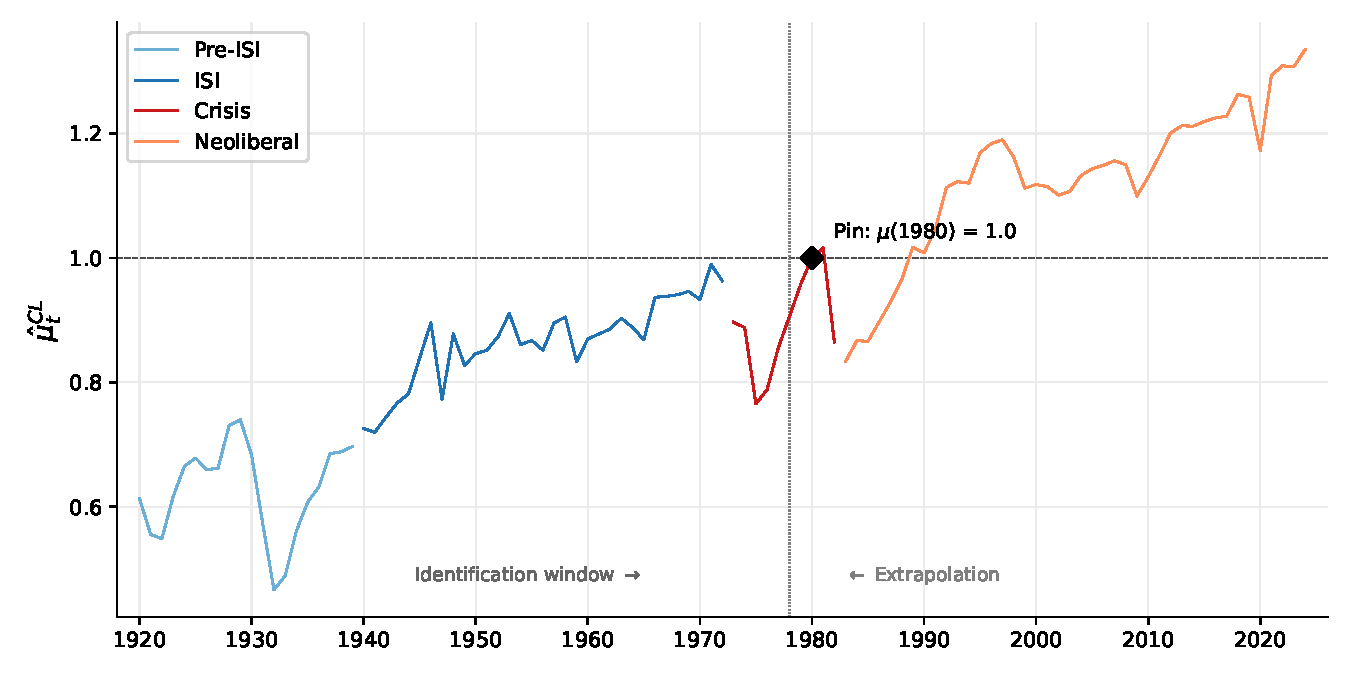
\includegraphics[width=\textwidth]{figures/fig4_mu_CL.pdf}
\end{figure}

\subsubsection{Stage B: Profitability Analysis --- Chile}
\label{sssec:stageB_cl}

% ---- Stage B Chile body --- written by analyst agent, 2026-04-09 ----

% -----------------------------------------------------------------------
% P1 --- Four-channel identity and analytical motivation
% -----------------------------------------------------------------------

The Chilean profit rate decomposes into the same four channels as the US
case --- but the structural position of each channel is governed by the
BoP constraint that US accumulation does not face. The four-channel
identity separates nominal capital productivity into its real-quantity
and relative-price components:
%
\begin{equation}
    r_t \;=\; \hat{\mu}_t \;\cdot\; \frac{P_Y}{P_K}\bigg|_t
              \;\cdot\; B_{r,t} \;\cdot\; \pi_t
    \label{eq:cl:4ch_identity}
\end{equation}
%
or in log-additive form:
%
\begin{equation}
    \Delta\ln r_t \;=\; \underbrace{\Delta\ln\hat{\mu}_t}_{\phi_\mu}
    \;+\; \underbrace{\Delta\ln(P_Y/P_K)_t}_{\phi_{p}}
    \;+\; \underbrace{\Delta\ln B_{r,t}}_{\phi_{B}}
    \;+\; \underbrace{\Delta\ln\pi_t}_{\phi_\pi}
    \label{eq:cl:4ch_log}
\end{equation}
%
where $B_{r,t} = B_t / (P_Y/P_K)_t$ recovers real capital productivity at
normal capacity by deflating nominal capital productivity by the
output-to-capital relative price. The analytical necessity of this
separation is more consequential for the peripheral case than for the
center. In an economy where capital goods are structurally import-dependent,
the price of capital relative to output is not a domestic relative price
governed primarily by productivity dynamics in the capital-goods sector: it
is a world-market transmission mechanism, modulated by the exchange rate and
the external balance position. A three-channel decomposition that retains
nominal $B_t$ conflates structural technology failure with world-market
price shocks that operate through the BoP-constrained import cost of
machinery and equipment. For Chile under ISI, where the external constraint
is the governing structural feature of accumulation, this conflation is not
merely a theoretical imprecision: it misattributes to productive stagnation
what this decomposition reads as world-market price dynamics transmitted
through the capital goods import channel.

% -----------------------------------------------------------------------
% Sub-period means --- Table B4
% -----------------------------------------------------------------------

\begin{table}[htbp]
\centering
\small
\caption{Weisskopf components: sub-period means, Chile, 1940--1978.}
\label{tab:B4_subperiod_CL}
\begin{threeparttable}
\begin{tabular}{llrrrrr}
\toprule
Period & Years & $\bar{r}$ & $\bar{\mu}$ & $\overline{Py/PK}$ & $\bar{B}_{r}$ & $\bar{\pi}$ \\
\midrule
Pre-ISI/WWII & 1940--1945 & 0.052 & 0.763 & 0.998 & 0.174 & 0.396 \\
\midrule
Early ISI & 1946--1953 & 0.068 & 0.857 & 1.084 & 0.172 & 0.425 \\
Mid ISI & 1954--1961 & 0.079 & 0.870 & 1.126 & 0.166 & 0.477 \\
Late ISI & 1962--1972 & 0.062 & 0.927 & 1.031 & 0.155 & 0.418 \\
\midrule
Crisis & 1973--1978 & 0.052 & 0.850 & 0.778 & 0.149 & 0.522 \\
\bottomrule
\end{tabular}
\begin{tablenotes}
\small
\item \textit{Notes:}
  Period arithmetic means of level variables.
  $r = \Pi/K$ (nominal profit rate);
  $\hat{\mu}$ from Stage~A MPF (capacity utilization);
  $Py/PK$ = GDP deflator / capital price deflator;
  $B_{r} = Y^{p}_{r}/K$ (real capital productivity at normal capacity);
  $\pi = \Pi/Y$ (profit share).
  Exact identity in levels: $r \equiv \hat{\mu} \cdot (Py/PK) \cdot B_{r} \cdot \pi$.
\end{tablenotes}
\end{threeparttable}
\end{table}


The sub-period level means in Table~\ref{tab:B4_subperiod_CL} trace the
macroscopic profile of the ISI arc and its termination. The nominal profit
rate rises from $\bar{r} = 0.052$ in the Pre-ISI/WWII sub-period
(1940--1945) to $\bar{r} = 0.068$ in the Early ISI (1946--1953), reaching
its peak at $\bar{r} = 0.079$ in the Mid ISI (1954--1961). The Late ISI
(1962--1972) registers a contraction to $\bar{r} = 0.062$, and the Crisis
sub-period (1973--1978) returns to $\bar{r} = 0.052$ --- the same level
as the WWII baseline. The ISI arc is therefore symmetric in its profit-rate
envelope: it rises for twenty years and contracts for the following
seventeen, with the macroscopic turning point locatable at the
mid-ISI--late-ISI transition in the early 1960s.

The channel-level means clarify which mechanisms sustained and then
exhausted the arc. The profit share $\bar{\pi}$ rises through the first
three sub-periods --- from $0.396$ to $0.425$ to $0.477$ --- consistent
with an accumulation regime in which deepening industrialization allowed
ISI capital to absorb a rising share of value added. Its compression in
the Late ISI ($\bar{\pi} = 0.418$) and apparent elevation in the Crisis
($\bar{\pi} = 0.522$, driven by coup-period wage suppression rather than
accumulation regime coherence) traces the distributional conflict that the
ISI arc could not resolve within its institutional architecture. The ISI arc
is $\pi$-dominant in its macroscopic structure: the profit rate tracks the
profit share more closely than any other channel across sub-periods.
Capacity utilization $\bar{\hat{\mu}}$ rises monotonically through the Late
ISI (from $0.763$ to $0.927$) --- consistent with the demand-activation
logic of the ISI arc --- yet that activation is insufficient to sustain the
profit rate once the profit share compresses. Real capital productivity
$\bar{B}_r$ declines across the full arc (from $0.174$ to $0.166$ to
$0.155$ to $0.149$), reflecting the progressive erosion of capital
efficiency as import-substitution opportunities were exhausted at each
technological tier. The $P_Y/P_K$ relative price rises through Mid ISI
($\overline{P_Y/P_K} = 1.126$) before compressing sharply in the Crisis
($\overline{P_Y/P_K} = 0.778$), capturing the capital-goods price shock
of the coup period and post-coup external adjustment.

% -----------------------------------------------------------------------
% Figure B1 panel --- six level series
% -----------------------------------------------------------------------

\begin{figure}[htbp]
    \centering
    \caption{Four-channel components: level series, Chile, 1940--1978.
    All series indexed to 1940\,=\,100.
    ISI sub-period bands shaded; BoP binding years (Regime~2,
    $ECT_{m,t-1} > -0.1394$) marked.}
    \label{fig:cl:B1}
    \begin{subfigure}[t]{0.48\textwidth}
        \centering
        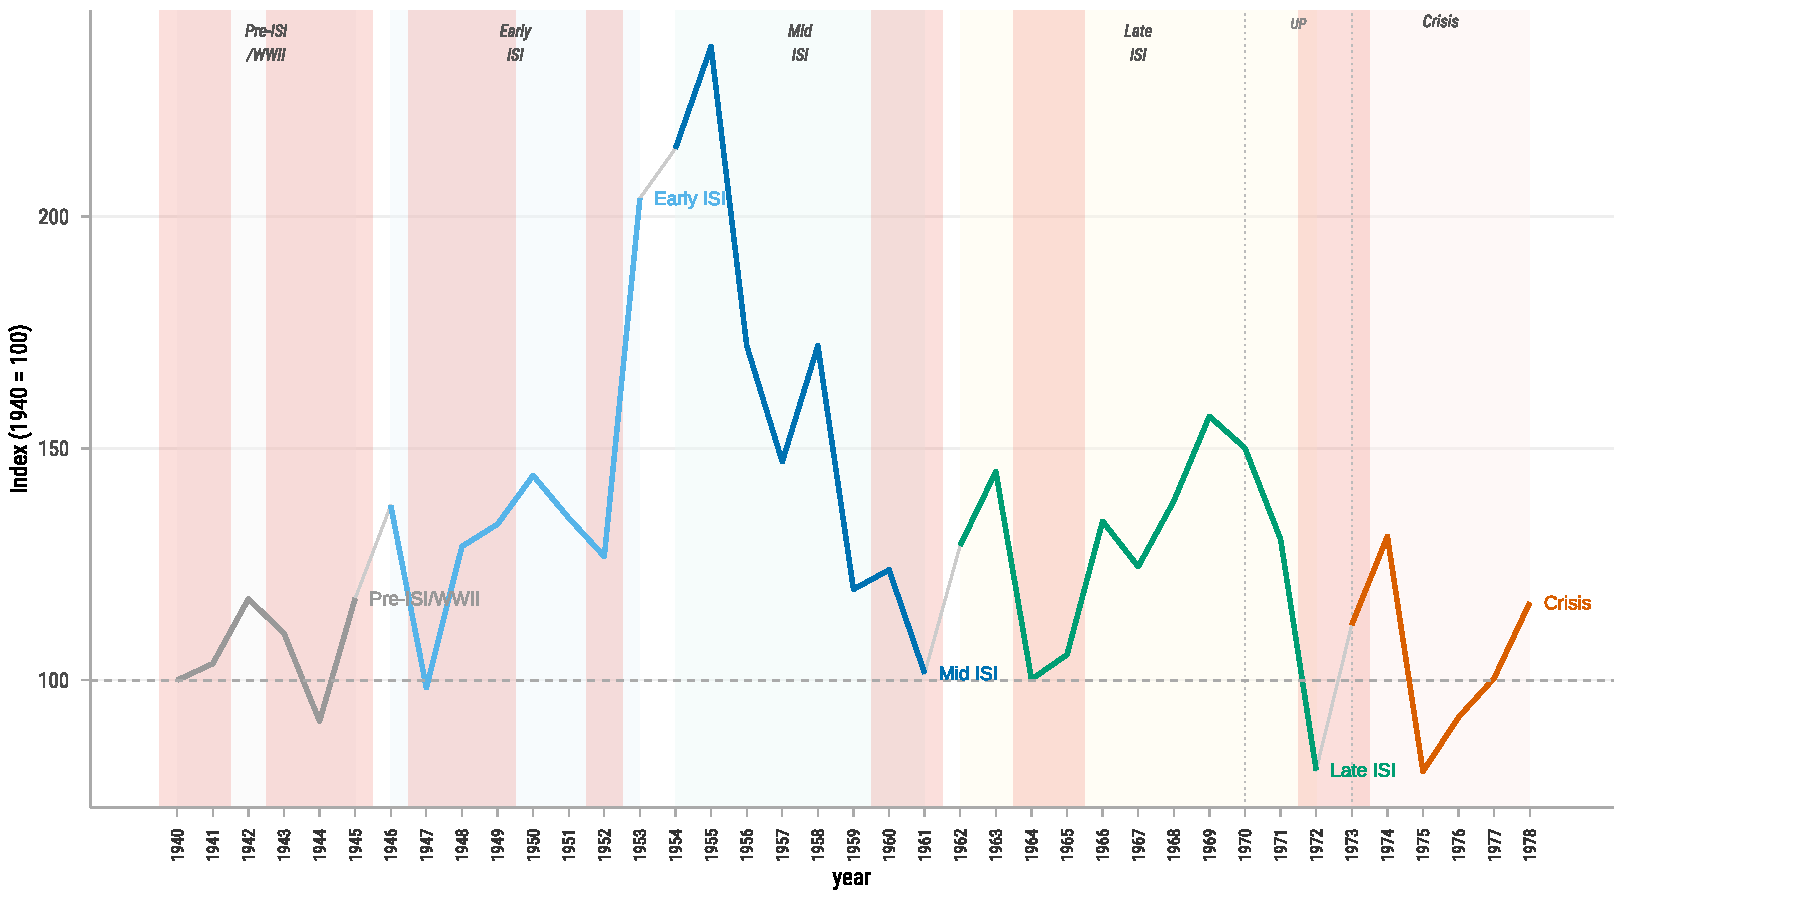
\includegraphics[width=\textwidth]{figures/fig_CL_B1a_r_levels}
        \caption{Profit rate $r_t = \Pi_t/K_t$.}
        \label{fig:cl:B1a}
    \end{subfigure}
    \hfill
    \begin{subfigure}[t]{0.48\textwidth}
        \centering
        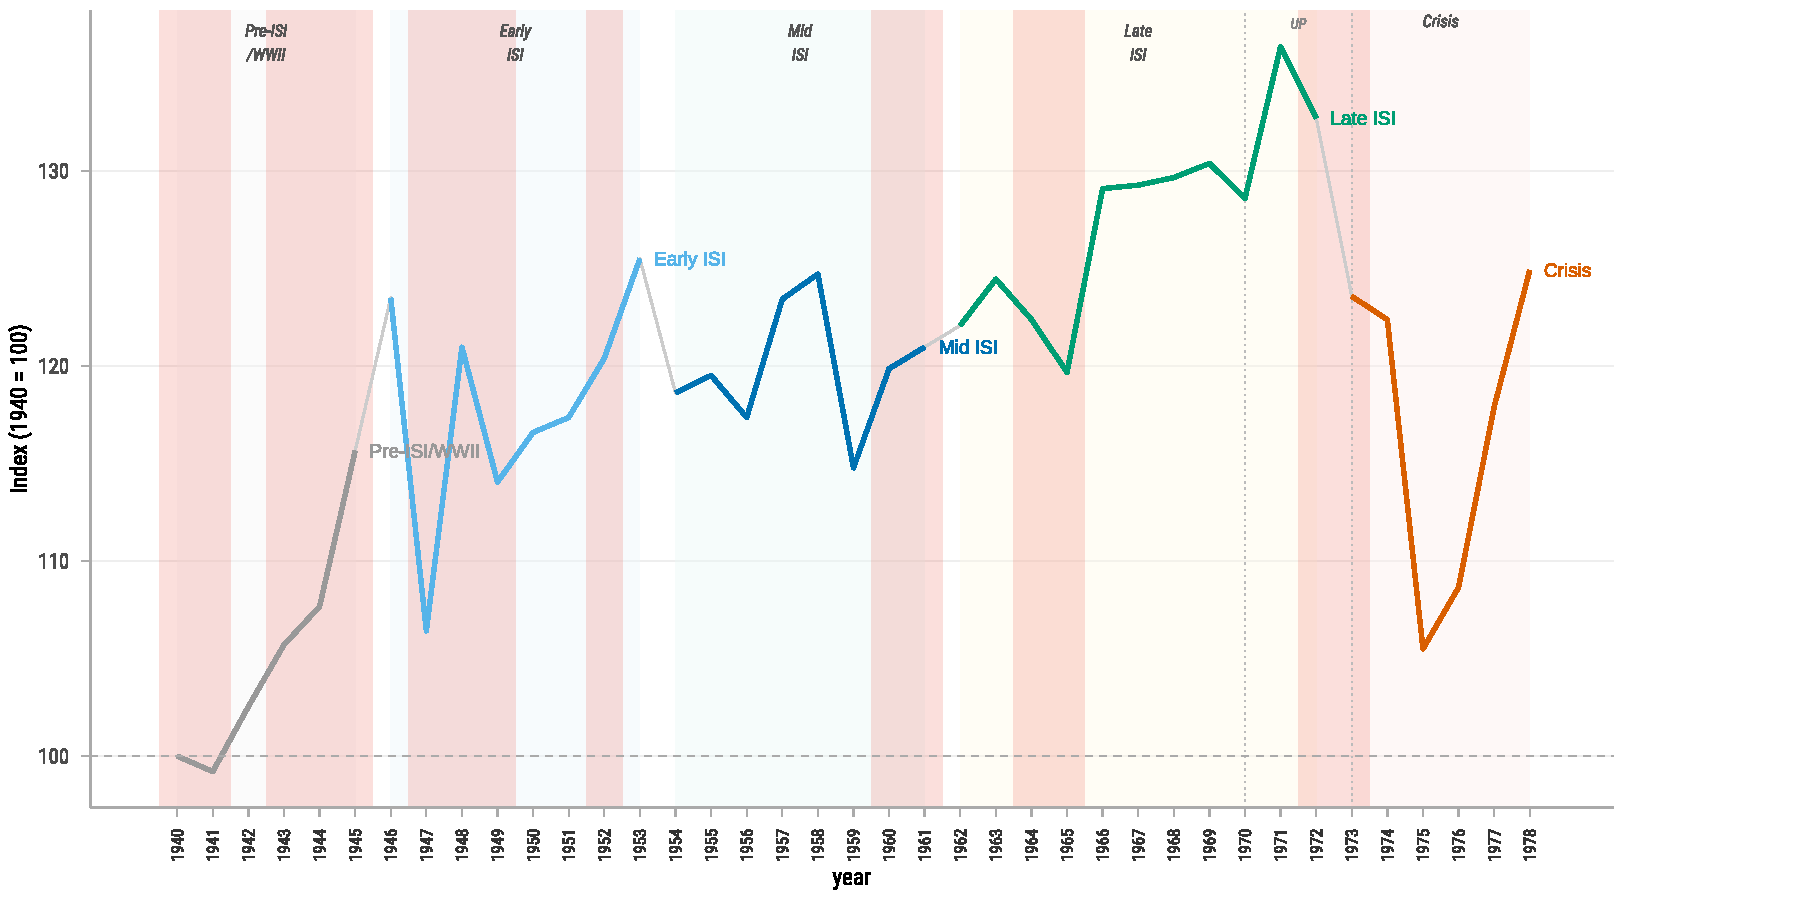
\includegraphics[width=\textwidth]{figures/fig_CL_B1b_mu_levels}
        \caption{Capacity utilization $\hat{\mu}_t$ (Stage~A MPF).}
        \label{fig:cl:B1b}
    \end{subfigure}
    \\[1em]
    \begin{subfigure}[t]{0.48\textwidth}
        \centering
        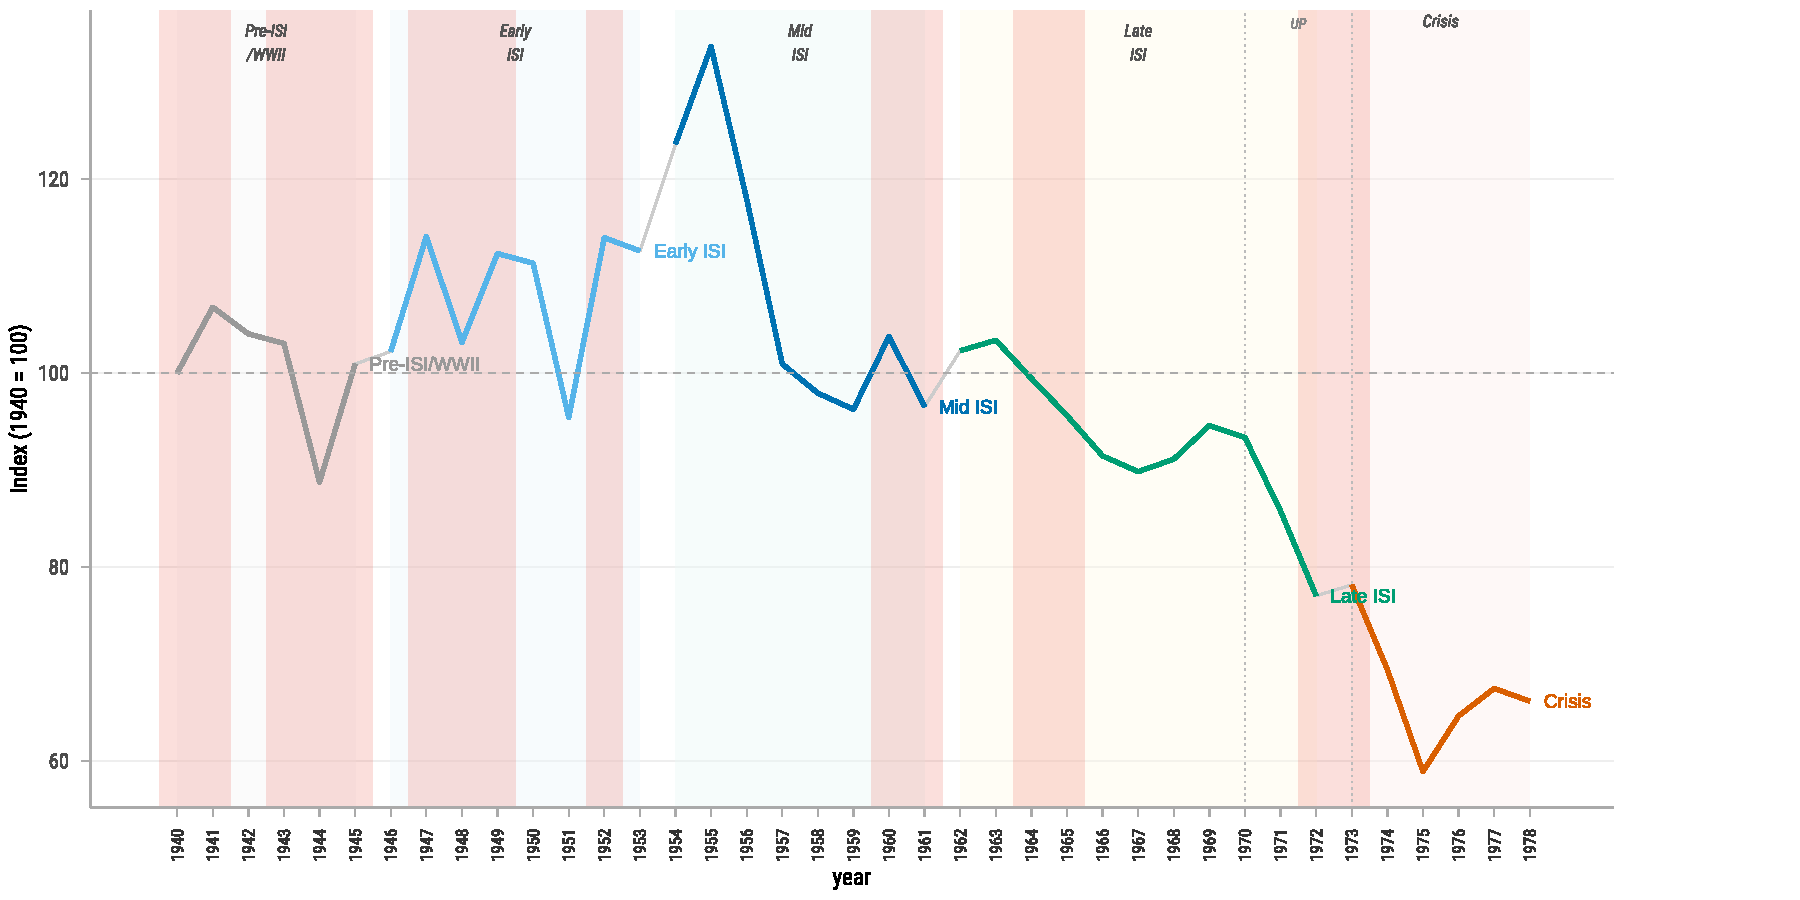
\includegraphics[width=\textwidth]{figures/fig_CL_B1c_B_levels}
        \caption{Nominal capital productivity $B_t$ (reference only).}
        \label{fig:cl:B1c}
    \end{subfigure}
    \hfill
    \begin{subfigure}[t]{0.48\textwidth}
        \centering
        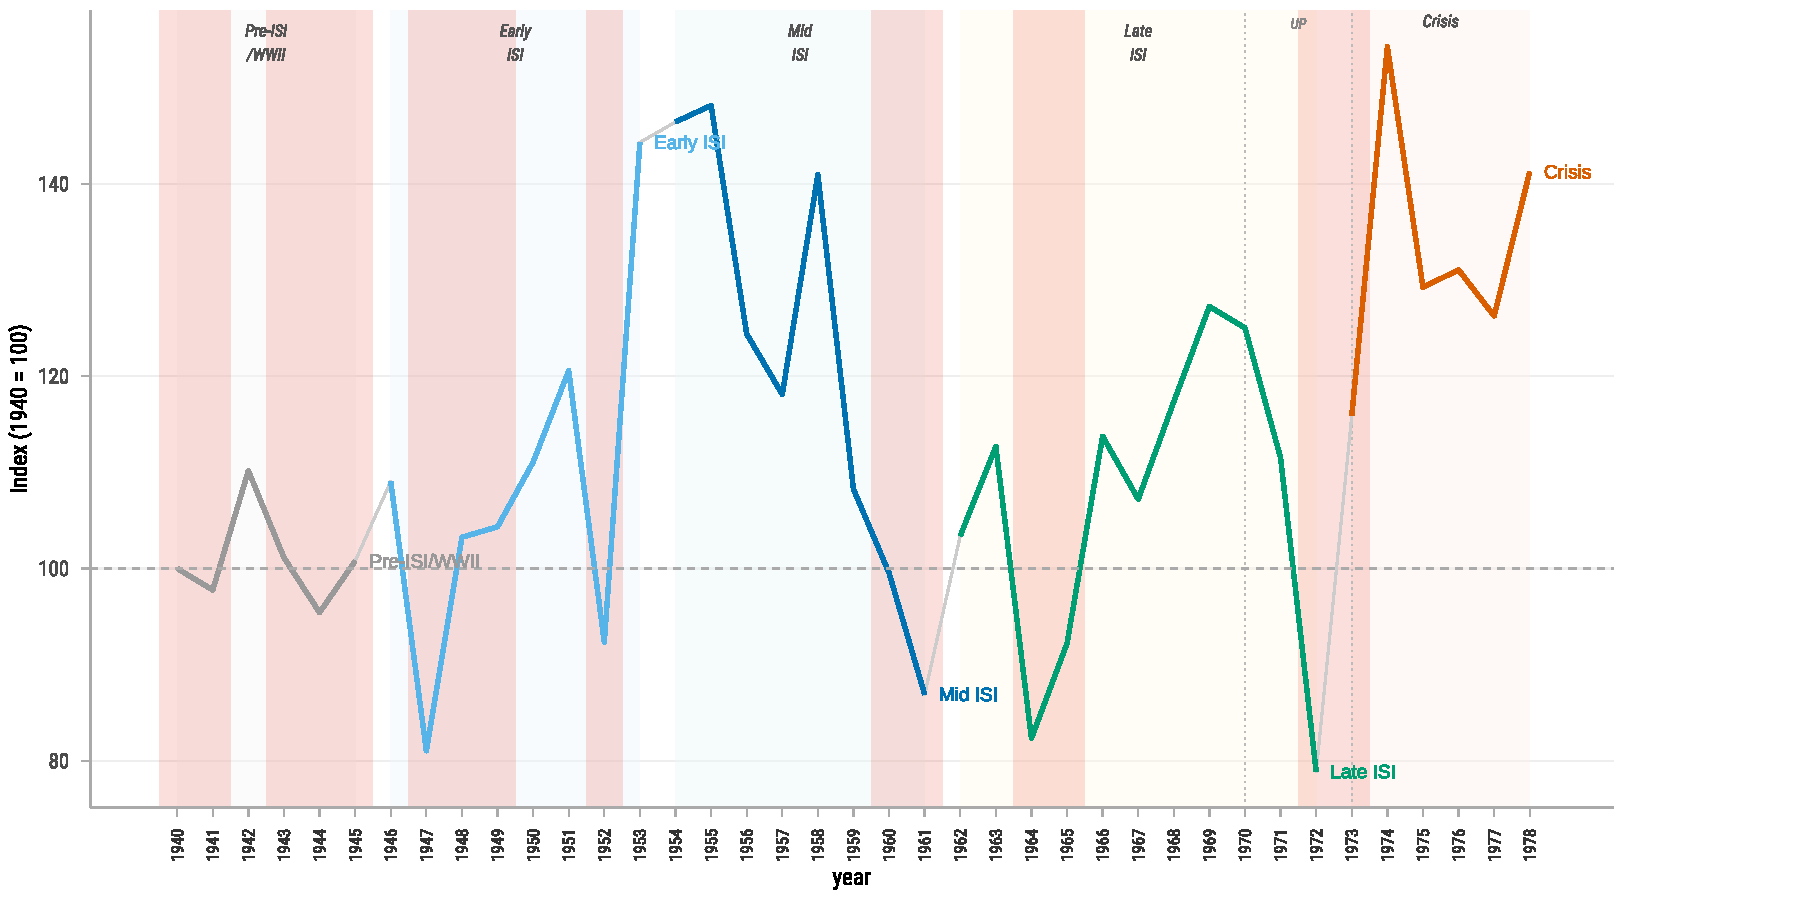
\includegraphics[width=\textwidth]{figures/fig_CL_B1d_pi_levels}
        \caption{Profit share $\pi_t = \Pi_t/Y_t$.}
        \label{fig:cl:B1d}
    \end{subfigure}
    \\[1em]
    \begin{subfigure}[t]{0.48\textwidth}
        \centering
        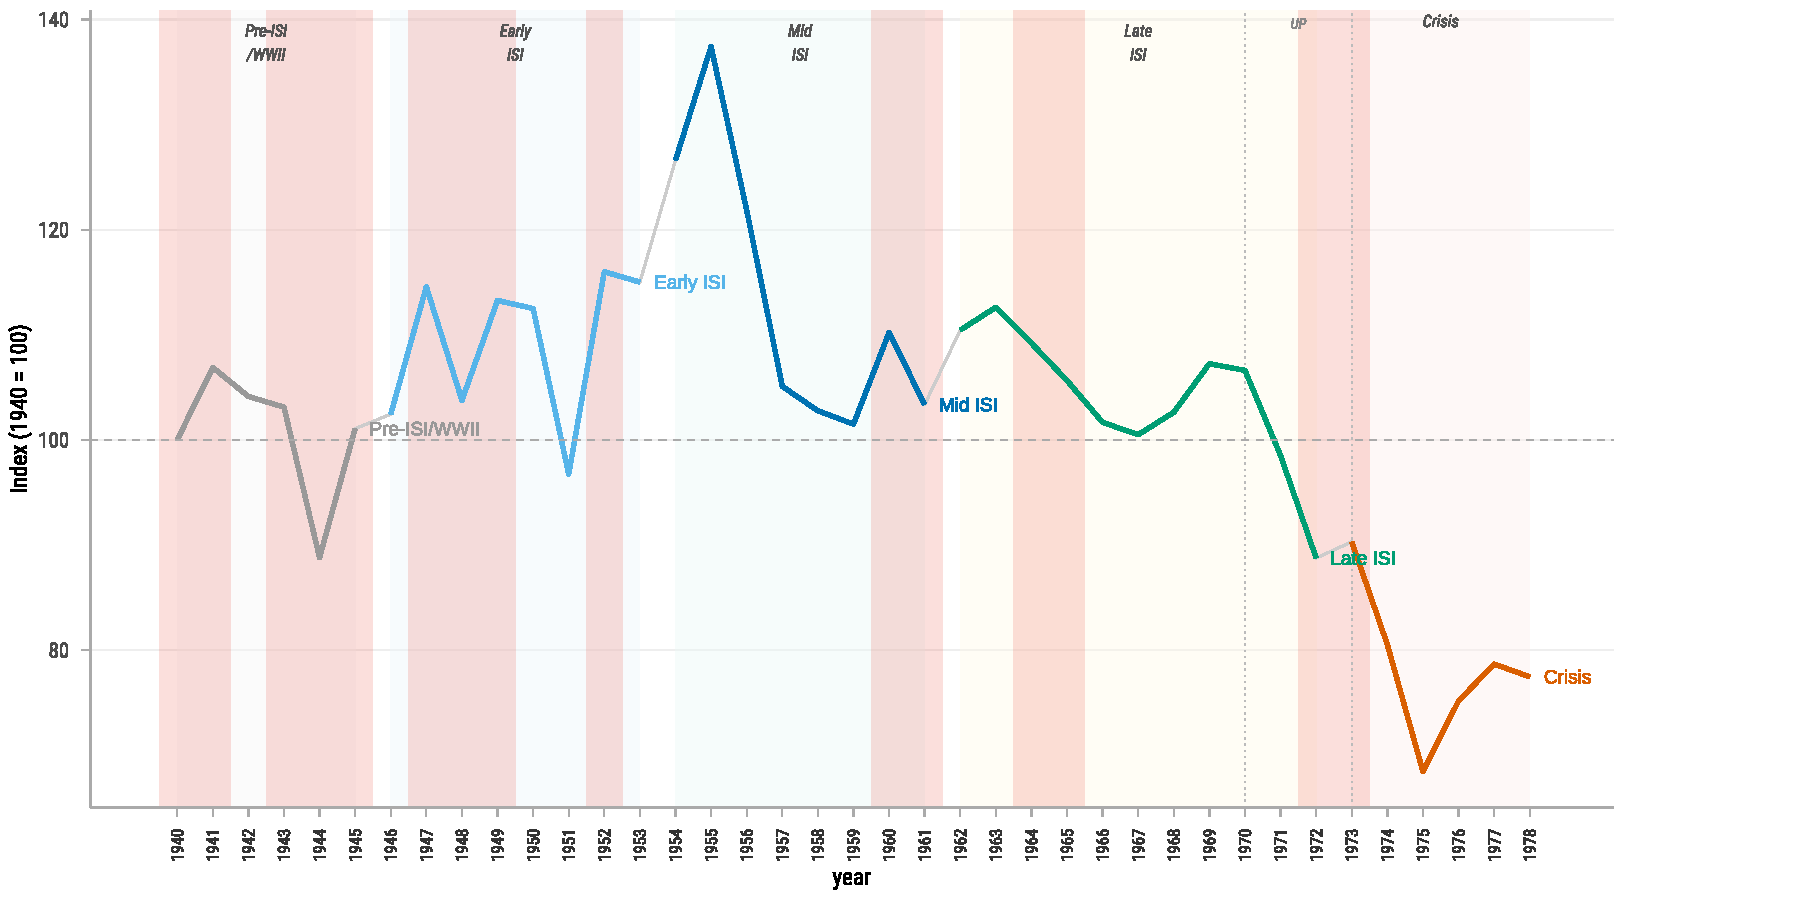
\includegraphics[width=\textwidth]{figures/fig_CL_B1e_PyPK_levels}
        \caption{Relative price $(P_Y/P_K)_t$.}
        \label{fig:cl:B1e}
    \end{subfigure}
    \hfill
    \begin{subfigure}[t]{0.48\textwidth}
        \centering
        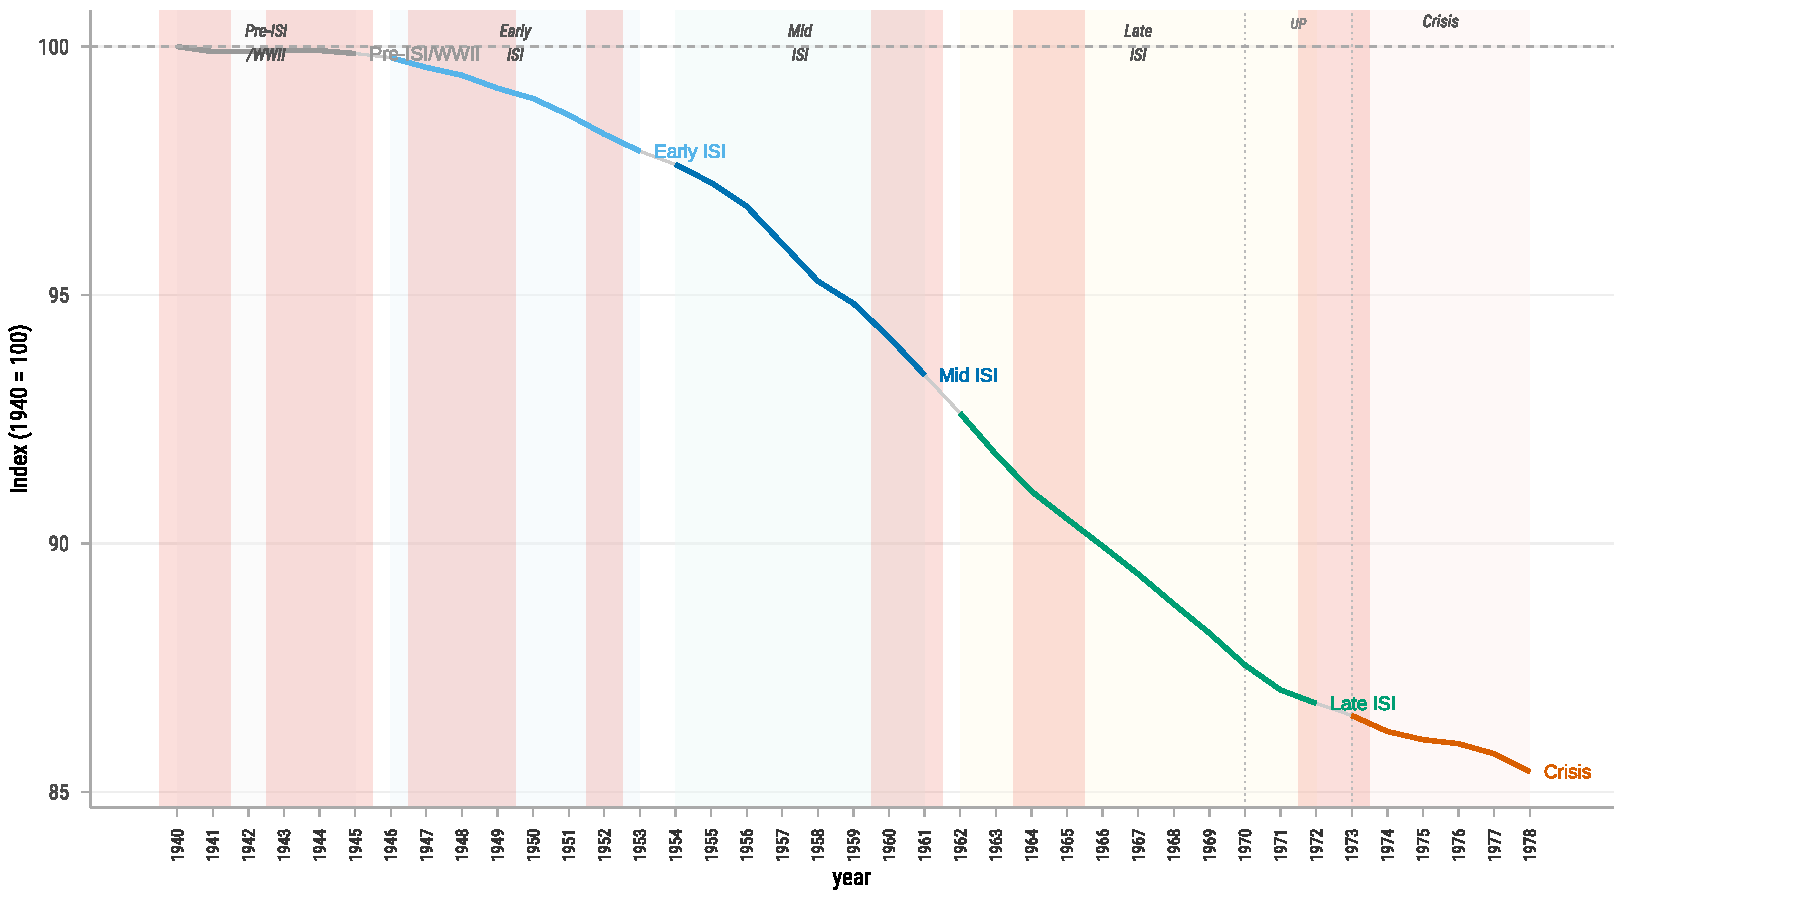
\includegraphics[width=\textwidth]{figures/fig_CL_B1f_Breal_levels}
        \caption{Real capital productivity $B_{r,t}$.}
        \label{fig:cl:B1f}
    \end{subfigure}
\end{figure}

% -----------------------------------------------------------------------
% Turning-point structure --- Tables B5 and Figure B4
% -----------------------------------------------------------------------

\begin{table}[htbp]
\centering
\small
\caption{Four-channel decomposition of profit-rate swings, Chile, 1940--1978.}
\label{tab:B5_peaktotrough_CL}
\begin{threeparttable}
\adjustbox{max width=\textwidth}{
\begin{tabular}{llrrrrrrrl}
\toprule
Period & Type & $\Delta\ln r$ & $s_{\mu}$ & $s_{Py/PK}$ & $s_{B_{r}}$ & $s_{\pi}$ & $\Sigma$ & Dominant \\
\midrule
1940-1946 & Expansion & +0.320 & 0.660 & 0.076 & \textit{-0.007}$^{\dagger}$ & 0.271 & 1.000 & $\mu$ \\
\addlinespace[3pt]
1946-1947 & Contraction & -0.336 & 0.443 & \textit{-0.333}$^{\dagger}$ & 0.006 & 0.884 & 1.000 & $\pi$ \\
\addlinespace[3pt]
1947-1953 & Expansion & +0.729 & 0.226 & 0.005 & \textit{-0.023}$^{\dagger}$ & 0.792 & 1.000 & $\pi$ \\
\addlinespace[3pt]
1953-1961 & Contraction & -0.698 & 0.053 & 0.153 & 0.068 & 0.727 & 1.000 & $\pi$ \\
\addlinespace[3pt]
1961-1969 & Expansion & +0.436 & 0.172 & 0.085 & \textit{-0.131}$^{\dagger}$ & 0.875 & 1.000 & $\pi$ \\
\addlinespace[3pt]
1969-1972 & Contraction & -0.666 & \textit{-0.027}$^{\dagger}$ & 0.284 & 0.024 & 0.718 & 1.000 & $\pi$ \\
\addlinespace[3pt]
1972-1974 & Expansion & +0.486 & \textit{-0.167}$^{\dagger}$ & \textit{-0.201}$^{\dagger}$ & \textit{-0.013}$^{\dagger}$ & 1.381$^{*}$ & 1.000 & $\pi$$^{*}$ \\
\addlinespace[3pt]
1974-1975 & Contraction & -0.490 & 0.303 & 0.332 & 0.004 & 0.362 & 1.000 & $\pi$ \\
\addlinespace[3pt]
1975-1978 & Expansion & +0.374 & 0.452 & 0.331 & \textit{-0.020}$^{\dagger}$ & 0.238 & 1.000 & $\mu$ \\
\bottomrule
\end{tabular}}
\begin{tablenotes}
\small
\item \textit{Notes:}
  $s_{j} = \varphi^{j}/\Delta\ln r$ (share of total compounded log-change);
  $s_{\mu} + s_{Py/PK} + s_{B_{r}} + s_{\pi} = 1$ (exact).
  $\varphi^{\mu} = \Delta\ln\hat{\mu}$,
  $\varphi^{Py/PK} = \Delta\ln(Py/PK)$,
  $\varphi^{B_{r}} = \Delta\ln B_{r}$,
  $\varphi^{\pi} = \Delta\ln\pi$.
\item[$\dagger$] Offsetting channel: contribution moves against the swing direction ($s_{j} < 0$).
\item[$*$] Share exceeds unity: channel more than accounts for total swing;
  remaining channels are jointly offsetting.
\end{tablenotes}
\end{threeparttable}
\end{table}


Figure~\ref{fig:cl:B4} identifies nine turning points in the profit rate
over the 1940--1978 window, organized into the nine profit-rate swings
whose channel composition Table~\ref{tab:B5_peaktotrough_CL} decomposes.
The turning-point structure of the Chilean profit rate follows a
qualitatively different periodization logic from the US case. Absent the
Fordist wage compromise and the military-Keynesian demand management
apparatus that organized US swing structure around the institutional
settlement's capacity to contain stagnation tendencies, Chilean profit-rate
turning points are governed by the BoP constraint periodization identified
in Stage~A. The external balance position --- registered as the threshold
regime indicator $ECT_{m,t-1}$ crossing $\hat{\gamma} = -0.1394$ ---
organizes the transition between expansion phases driven by ISI
demand-activation and contraction phases driven by distributional
compression or external adjustment. The nine swings span three structurally
distinct arcs: the pre-ISI demand-activation phase (1940--1947), the ISI
core governed by distributional conflict and its BoP-mediated resolution
(1947--1972), and the crisis and post-crisis restructuring period
(1972--1978).

% -----------------------------------------------------------------------
% Figure B4 --- profit rate with turning points
% -----------------------------------------------------------------------

\begin{figure}[htbp]
    \centering
    \caption{Profit rate with identified turning points, Chile, 1940--1978.
    Turning points identified on $r_t = \Pi_t/K_t$.
    ISI sub-period bands shaded; BoP binding years (Regime~2,
    $ECT_{m,t-1} > -0.1394$) marked by grey fill.}
    \label{fig:cl:B4}
    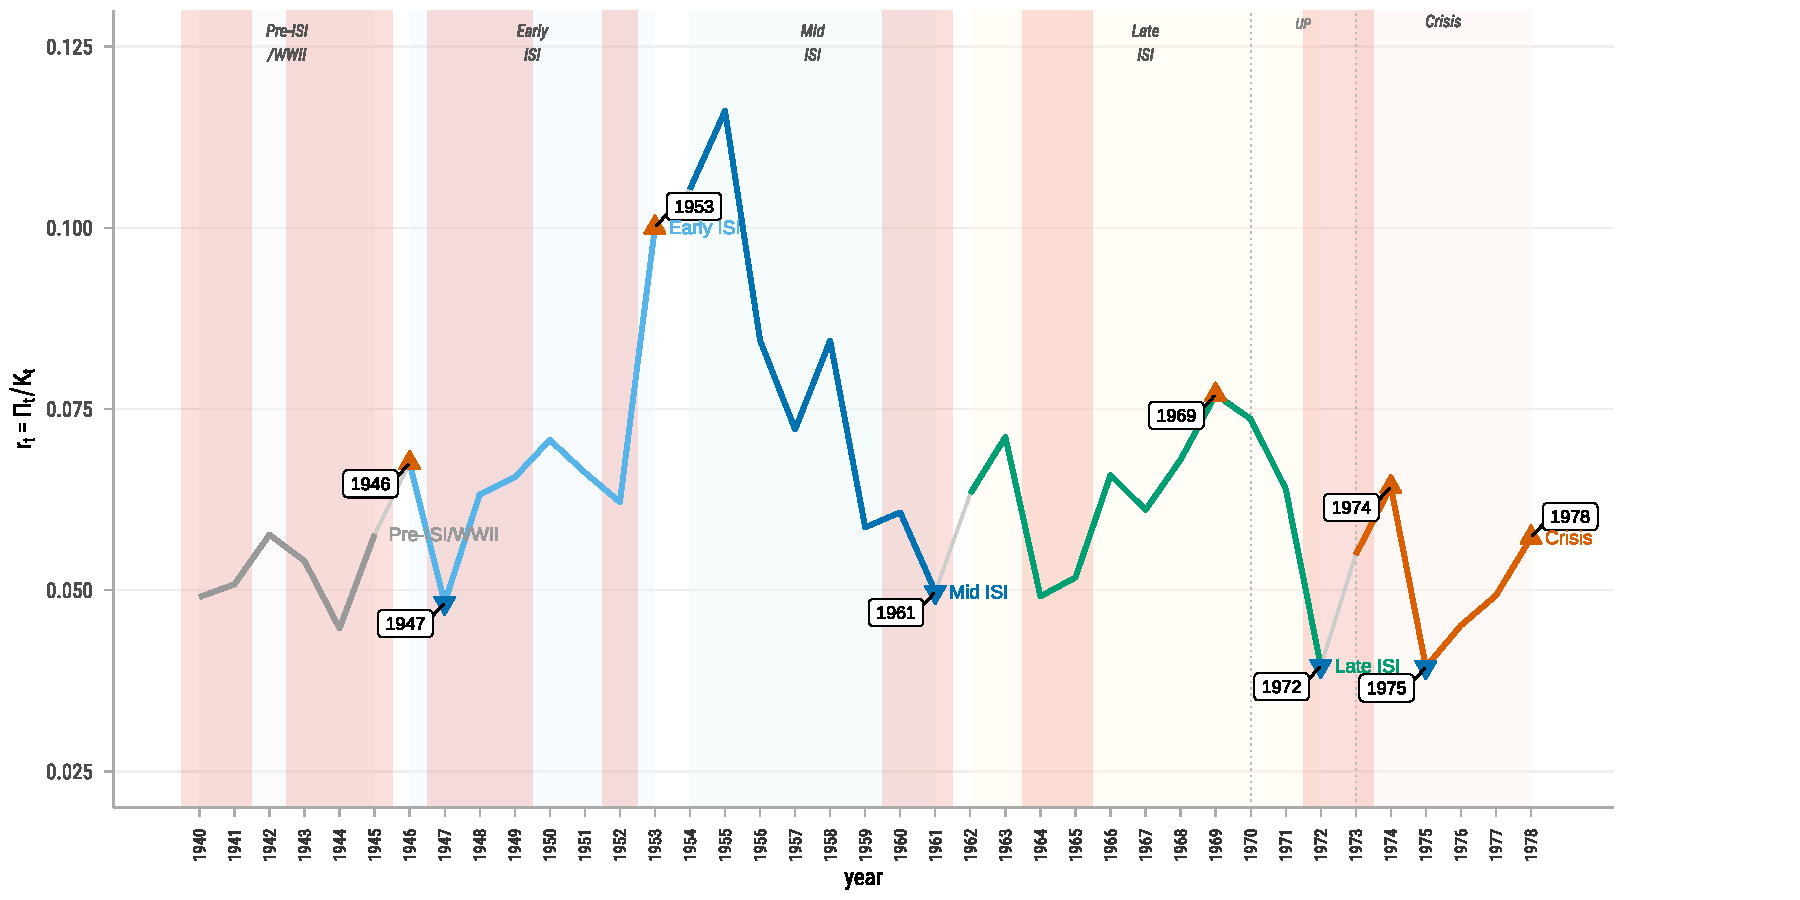
\includegraphics[width=\textwidth]{figures/fig_CL_B4_profit_rate_turning_points}
\end{figure}

% -----------------------------------------------------------------------
% Swing-by-swing analysis
% -----------------------------------------------------------------------

\paragraph{1940--1946 expansion.}

The first profit-rate swing ($\Delta\ln r = +0.320$) is the sole
pre-ISI episode and the first of two swings in which the capacity
utilization channel $\hat{\mu}$ furnishes the dominant contribution
($s_\mu = 0.660$). The mechanism is structural demand-activation: as ISI
industrialization begins to mobilize previously idle productive capacity
across the early-industrial sectors, actual activation of installed capacity
rises faster than the profit share adjusts. The profit share contributes
the secondary role ($s_\pi = 0.271$), consistent with an early accumulation
phase in which the distributional configuration has not yet been contested
at the frontier of labor-market bargaining. The $Py/PK$ channel contributes
a minor positive share ($s_{Py/PK} = 0.076$), and real capital productivity
is marginally offsetting ($s_{Br} = -0.007$), registering the early-ISI
condition in which the capital stock is being activated more rapidly than
its real productivity at normal capacity rises. This swing is not a
demand-pull expansion in the Keynesian sense: it is the structural response
of capacity utilization to the demand-activation properties of
import-substitution at the first tier of industrial reorganization.

\paragraph{1946--1947 contraction.}

The sharpest one-year decline in the series ($\Delta\ln r = -0.336$)
provides the first signal of the distributional conflict that will govern
the ISI arc. The profit share accounts for $s_\pi = 0.884$ of the decline
--- near-total distributional dominance in a single-year episode. The
$Py/PK$ channel is sharply offsetting ($s_{Py/PK} = -0.333$), meaning that
the relative price of output to capital moved in the profit-sustaining
direction, partially arresting the distributional compression. Capacity
utilization contributes $s_\mu = 0.443$, registering a demand-side pullback
coincident with the distributional pressure. The episode is analytically
interpretable as the first BoP-crisis signal: the tightening of external
balance conditions after wartime demand conditions recede transmits through
distributional conflict --- wage pressure at the import-dependent margin of
the industrial wage bill --- rather than through a technology shock or a
clean demand collapse.

\paragraph{1947--1953 expansion.}

The largest expansion in the series by compounded log-change ($\Delta\ln r
= +0.729$) is $\pi$-dominant with $s_\pi = 0.792$. The distributional
reconstitution of the profit share --- following the 1946--1947 compression
--- drives the recovery. The capacity utilization channel contributes
$s_\mu = 0.226$, registering renewed demand-activation as the Early ISI
industrial push consolidates. The $Py/PK$ and $B_r$ channels are
approximately neutral ($s_{Py/PK} = 0.005$, $s_{Br} = -0.023$). This is
the clearest single-channel $\pi$-governed expansion in the series: the
recovery is primarily a distributional correction, not a technology advance
or a demand surge, and the BoP constraint periodization places the expansion
in Regime~1 (slack) years that afford space for distributional reconstitution
without immediate external adjustment pressure.

\paragraph{1953--1961 contraction.}

The longest contraction by duration ($\Delta\ln r = -0.698$ over eight
years) is again $\pi$-dominant ($s_\pi = 0.727$). The sustained compression
of the profit share across the late Early ISI into the Mid ISI reflects the
progressive exhaustion of the first ISI tier's distributional settlement:
as labor-market bargaining strengthens alongside the maturation of the
industrial wage bill, the profit share faces structural downward pressure
that demand reactivation ($s_\mu = 0.053$, minor) and relative-price
improvement ($s_{Py/PK} = 0.153$, partial offset) cannot counteract. Real
capital productivity contributes $s_{Br} = 0.068$ to the contraction,
meaning $B_r$ is declining with the profit rate. This is not a
technology-led crisis; it is a distributional compression that the ISI
regime's capacity for productivity upgrading cannot outrun at this
technological tier.

\paragraph{1961--1969 expansion.}

The Late ISI expansion ($\Delta\ln r = +0.436$) is the most
technology-constrained of the $\pi$-dominant expansions. The profit share
accounts for $s_\pi = 0.875$ --- the largest $\pi$-share of any expansion
in the series --- but real capital productivity is a structural headwind
($s_{Br} = -0.131$, offsetting). The four-channel decomposition makes
visible a mechanism that the three-channel framework would absorb entirely
into the nominal capital productivity signal: $B_r$ is declining at normal
capacity even as the profit rate recovers, meaning that the recovery is
purely distributional and demand-activated rather than productivity-grounded.
The $Py/PK$ channel contributes a modest positive share ($s_{Py/PK} =
0.085$), and capacity utilization furnishes $s_\mu = 0.172$. The Late ISI
expansion is not a balanced multi-channel recovery: it is a distributional
and demand push against a declining real productive capacity --- the
structural configuration that the BoP-constrained exhaustion of ISI generates
as each technological tier approaches saturation.

\paragraph{1969--1972 contraction.}

The pre-coup profit-rate compression ($\Delta\ln r = -0.666$) is
$\pi$-dominant ($s_\pi = 0.718$) with a distinctive secondary structure.
The $Py/PK$ channel contributes $s_{Py/PK} = 0.284$ --- the second-largest
contributor --- registering the structural deterioration of the
output-to-capital relative price as the import cost of capital goods rises
and domestic output prices are constrained by late-ISI competitive pressures.
The capacity utilization channel is marginally offsetting ($s_\mu = -0.027$),
indicating that demand conditions were not contracting but mildly expanding,
consistent with the late-Frei and early-Allende demand stimulus. Real
capital productivity contributes a minor positive share ($s_{Br} = 0.024$)
to the contraction. The mechanism is therefore a distributional compression
amplified by a world-market price shock through the capital goods import
channel --- not a demand failure --- and the four-channel decomposition is
necessary to separate these two contributions.

\paragraph{1972--1974 expansion (Unidad Popular and coup).}

The most analytically distinctive result in the Chile Stage~B decomposition
concerns the expansion that spans the Unidad Popular's final year and the
first year of the Pinochet dictatorship ($\Delta\ln r = +0.486$,
1972--1974). The profit share accounts for $s_\pi = 1.381$ --- a share
exceeding unity --- constituting distributional overdetermination: the
$\pi$-channel alone more than accounts for the total compounded log-change
in the profit rate. The three remaining channels are jointly offsetting:
capacity utilization contributes $s_\mu = -0.167$, the $Py/PK$ relative
price $s_{Py/PK} = -0.201$, and real capital productivity $s_{Br} = -0.013$.

The mechanism requires interpretation against the BoP regime structure
established in Stage~A. The Unidad Popular years (1970--1972) fall entirely
in Regime~1 (BoP slack, $ECT_{m,t-1} \leq -0.1394$); the terminal year
(1974) falls in Regime~2 (BoP binding). The expansion therefore spans a
regime boundary, and the profit share channel records the distributional
consequence of that crossing. Under UP, the redistribution of surplus
toward labor --- wage increases and social expenditure financed through
monetary emission --- compressed the real wage-goods supply and accelerated
inflation; by 1972--1973 the resulting distributional crisis was resolved
by the coup rather than by institutional reconfiguration within the economic
mechanism. The $s_\pi = 1.381$ is not the expression of a functional
distributional settlement sustaining profitability: it is the arithmetic
registration of the fact that coup-period wage compression --- implemented
through political-military force --- raised the profit share by more than
the demand destruction ($s_\mu = -0.167$) and capital-goods price shock
($s_{Py/PK} = -0.201$) reduced it. Remove the $\pi$-channel and the
remaining three channels would have produced a profit-rate contraction, not
an expansion. The UP episode registers the distributional overdetermination
that is structurally specific to a peripheral economy whose chronic
over-accumulation tendency ($\hat{\theta}^{CL} < 1$ throughout, no
distributionally achievable under-accumulation configuration) concentrates
the resolution of distributional conflict into a single, politically
determined break rather than absorbing it through the regime alternation
that the US Fordist settlement institutionalized.

\paragraph{1974--1975 contraction (coup and shock therapy).}

The post-coup contraction ($\Delta\ln r = -0.490$) presents the most
analytically complex channel configuration in the series. Unlike every
other contraction, in which a single channel accounts for more than 70\%
of the compounded decline, the 1974--1975 episode distributes the
explanation across three channels at near-comparable weight: $s_{Py/PK} =
0.332$, $s_\mu = 0.303$, and $s_\pi = 0.362$, with real capital
productivity negligible ($s_{Br} = 0.004$). The coup-period contraction
operated simultaneously through two distinct transmission mechanisms.
Demand destruction --- the collapse of fiscal expenditure under shock
therapy, the suppression of real wages and consumption capacity ---
compressed capacity utilization and accounts for the $\mu$-channel
contribution. The capital-goods price shock --- the combined effect of
import liberalization raising the relative cost of internationally-priced
capital equipment and post-coup external adjustment forcing realignment of
the $Py/PK$ ratio --- transmits the world-market stagnation tendency through
the price channel. The four-channel identity separates these two mechanisms;
the three-channel nominal framework would merge them into an undifferentiated
capital productivity deterioration. The absence of single-channel dominance
is structurally informative: the 1974--1975 crisis is not resolvable through
a partial-channel correction but requires simultaneous reconfiguration of
the demand, distribution, and price environments.

\paragraph{1975--1978 expansion (neoliberal capacity reactivation).}

The terminal expansion ($\Delta\ln r = +0.374$) returns to the
demand-activation configuration of the 1940--1946 pre-ISI swing:
$\hat{\mu}$ accounts for $s_\mu = 0.452$ and $Py/PK$ for $s_{Py/PK} =
0.331$, with $\pi$ contributing only $s_\pi = 0.238$ and $B_r$ marginally
offsetting ($s_{Br} = -0.020$). The mechanism is capacity reactivation
under neoliberal restructuring: the suppression of domestic wages and the
elimination of ISI-era regulatory barriers reactivated idle productive
capacity by restoring the demand composition that capital goods utilization
required, while the post-liberalization exchange rate realignment improved
$Py/PK$. The $\mu$-channel dominance here does not register structural
regime change: consistent with the Stage~A theoretical clarification,
$\hat{\mu}$ captures the short-run deviation from the long-run
over-accumulation path, not the path itself. The demand-activation is
transitional and bounded, not a return to the ISI distributional settlement.

% -----------------------------------------------------------------------
% Figure B2 --- cumulative and annual contributions
% -----------------------------------------------------------------------

\begin{figure}[htbp]
    \centering
    \caption{Annual and cumulative four-channel contributions to
    $\Delta\ln r_t$, Chile, 1940--1978.}
    \label{fig:cl:B2}
    \begin{subfigure}[t]{\textwidth}
        \centering
        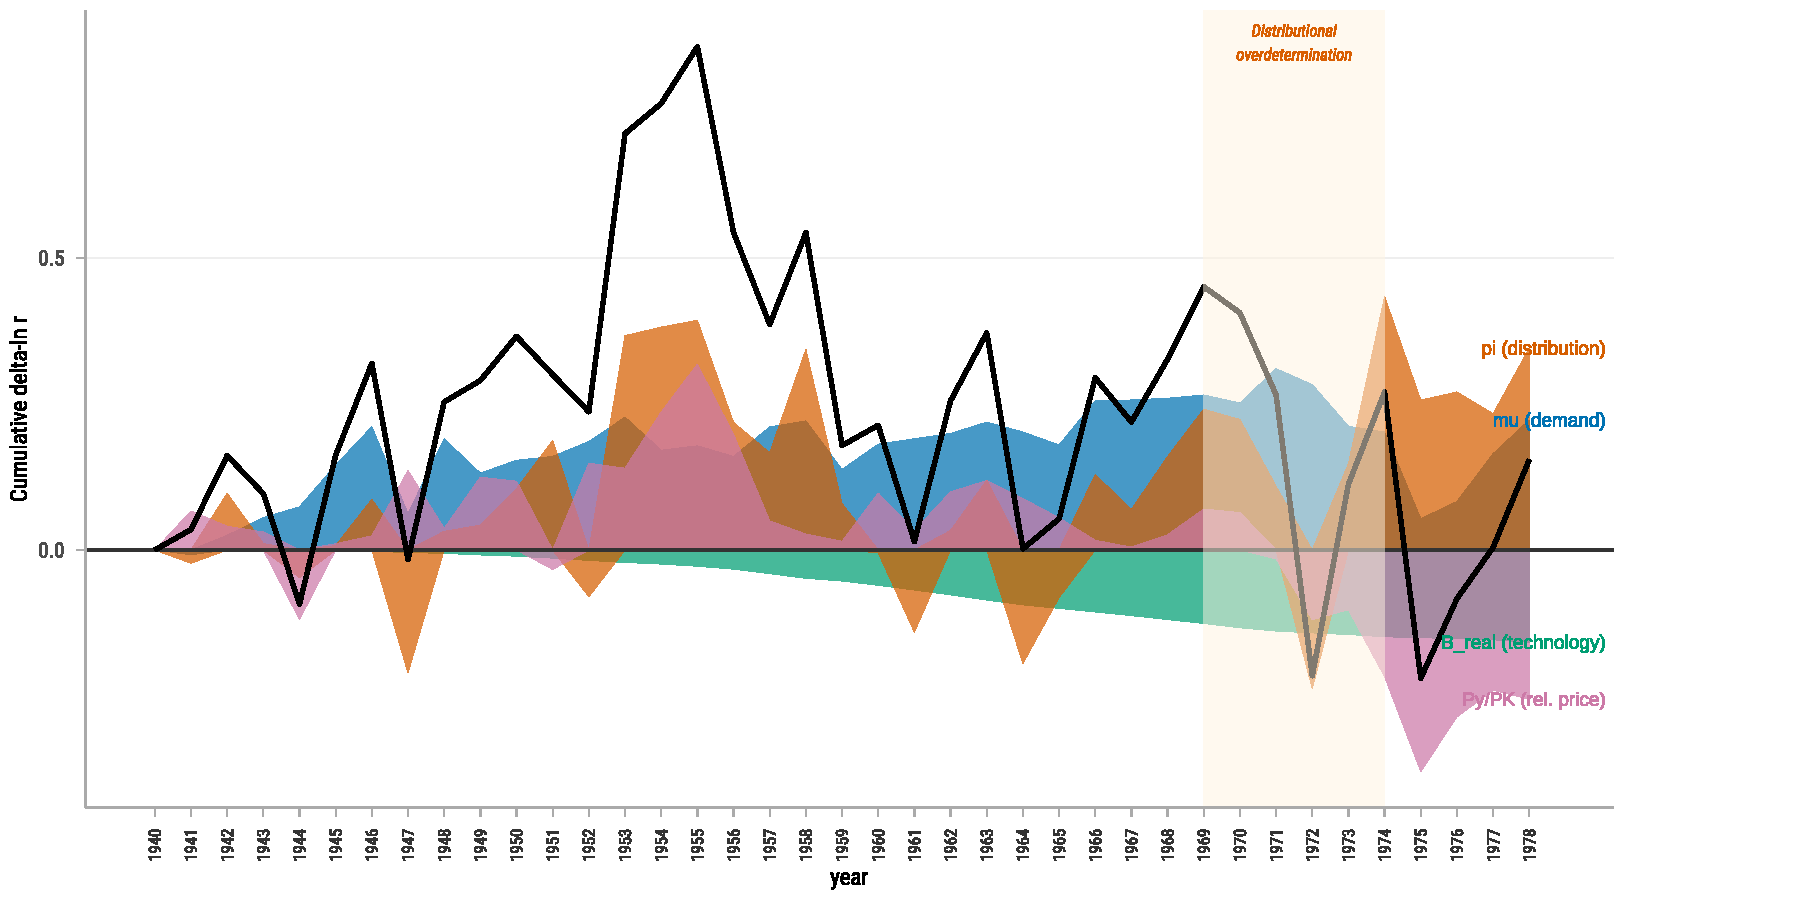
\includegraphics[width=\textwidth]{figures/fig_CL_B2a_cumulative}
        \caption{Cumulative log-change contributions.}
        \label{fig:cl:B2a}
    \end{subfigure}
    \\[1em]
    \begin{subfigure}[t]{\textwidth}
        \centering
        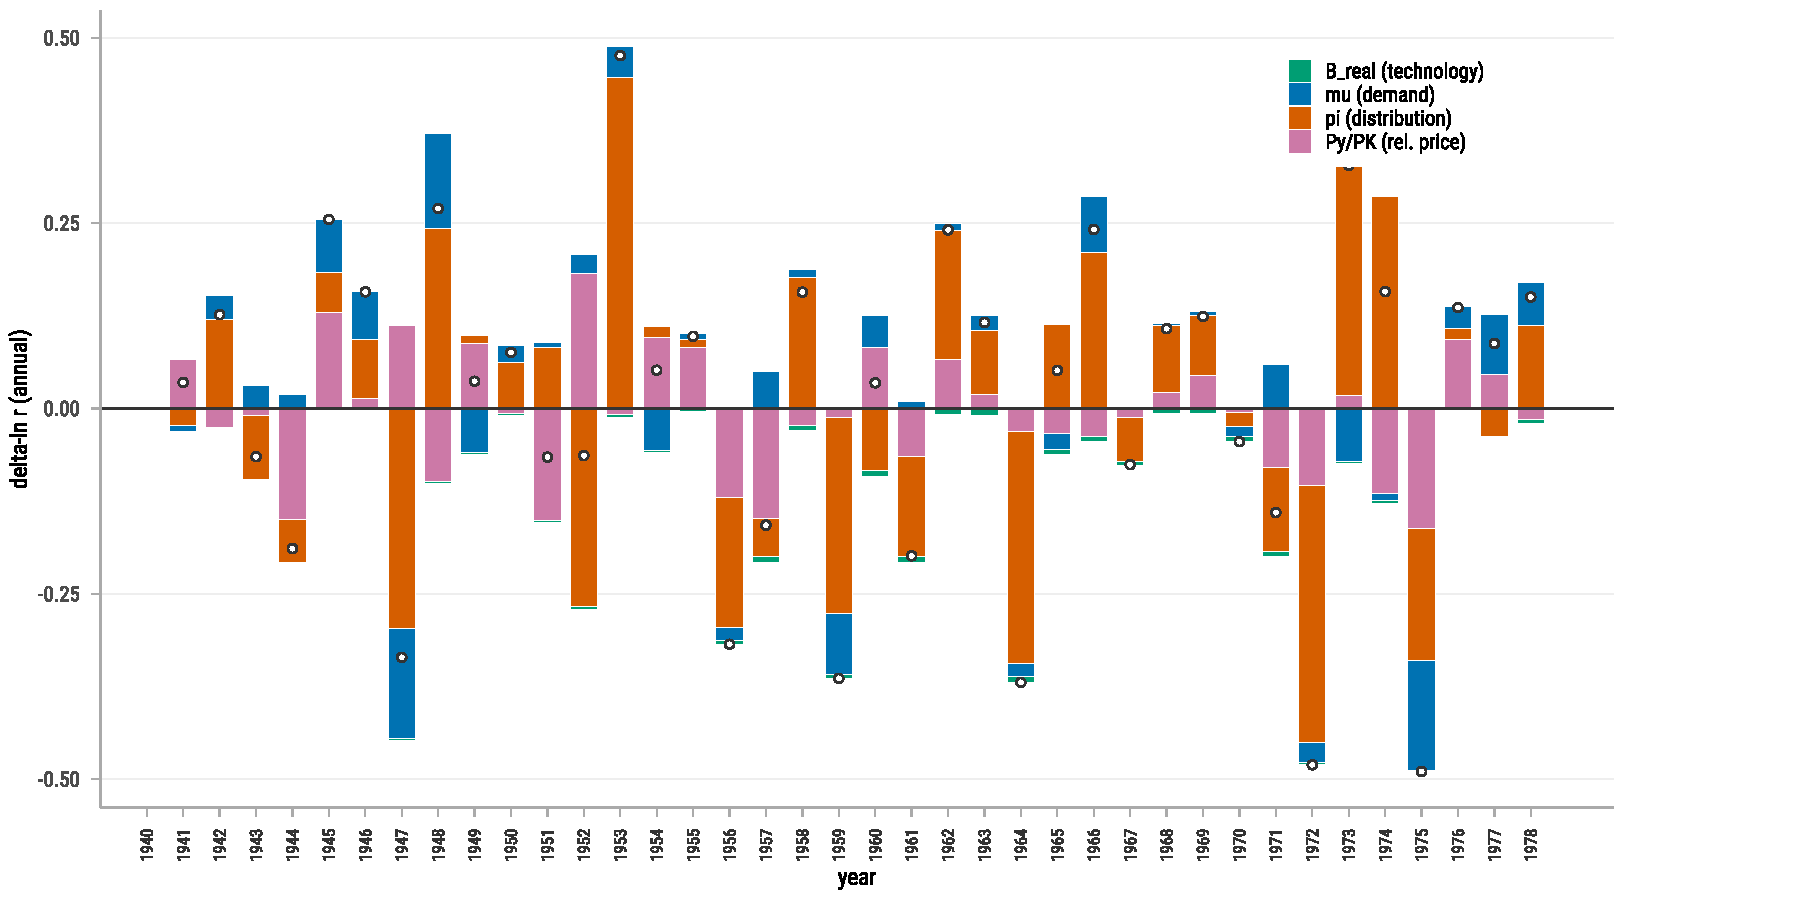
\includegraphics[width=\textwidth]{figures/fig_CL_B2b_annual_bars}
        \caption{Annual stacked-bar contributions.}
        \label{fig:cl:B2b}
    \end{subfigure}
\end{figure}

% -----------------------------------------------------------------------
% Synthesis
% -----------------------------------------------------------------------

Figure~\ref{fig:cl:B3} displays the channel composition of all nine
profit-rate swings. The $\pi$-channel registers as dominant in seven of
the nine swings, confirming the standard result of the distributional
framework for the Chilean case: the surplus distribution between capital
and labor is the primary determinant of profit-rate dynamics across the
ISI arc \citep{Weisskopf1979}. The two exceptions --- 1940--1946 and
1975--1978, both $\mu$-dominant --- are not randomly distributed across
the series. They bookend the ISI arc at precisely its demand-activation
margins: the pre-ISI demand-activation phase that precedes the
distributional contest of the industrialization core, and the post-crisis
capacity reactivation that follows the coup-period distributional resolution.
The $\mu$-dominance of these two swings registers a structural logic
consistent with the theorization of peripheral accumulation under the BoP
constraint: demand-activation is operative when the distributional
configuration has not yet been contested at the frontier of bargaining
(pre-ISI) or when the distributional contest has been forcibly resolved by
political violence and the only available margin of accumulation is idle
capacity reactivation (post-coup). In both cases, $\mu$-dominance is
transitional and bounded --- the ISI arc proper is $\pi$-governed
throughout, from the Early ISI distributional contest of 1946--1947 through
the Late ISI multi-channel compression of 1969--1972.

The 1972--1974 distributional overdetermination episode ($s_\pi = 1.381$)
is unique in the series and unique to the political economy of the Unidad
Popular. No other swing in the Chilean or US series records a channel share
exceeding unity with the remaining channels jointly offsetting. Its
structural interpretation --- grounded in the Stage~A regime classification
and the chronic over-accumulation identification --- is that it registers a
distributional rupture whose resolution was external to the economic
mechanism, requiring the political-military violence of the coup to
accomplish what institutional reconfiguration could not. This is the
empirical content of the theoretical claim that $\hat{\theta}^{CL} < 1$
throughout the ISI arc with no distributionally achievable under-accumulation
relief: distributional conflict accumulates beyond the capacity of the
institutional architecture to absorb it, resolving through a structural
break of a qualitatively different character from the regime alternation
that the US Fordist settlement institutionalized.

% -----------------------------------------------------------------------
% Figure B3 --- swing composition bar chart
% -----------------------------------------------------------------------

\begin{figure}[htbp]
    \centering
    \caption{Channel composition of profit-rate swings, Chile, 1940--1978.
    Shares $s_j = \varphi^j / \Delta\ln r$ (exact). Bars extending beyond
    $\pm 1$ indicate offsetting channels. $\dagger$ = offsetting channel;
    $^{*}$ = distributional overdetermination ($s_\pi > 1$, 1972--1974).}
    \label{fig:cl:B3}
    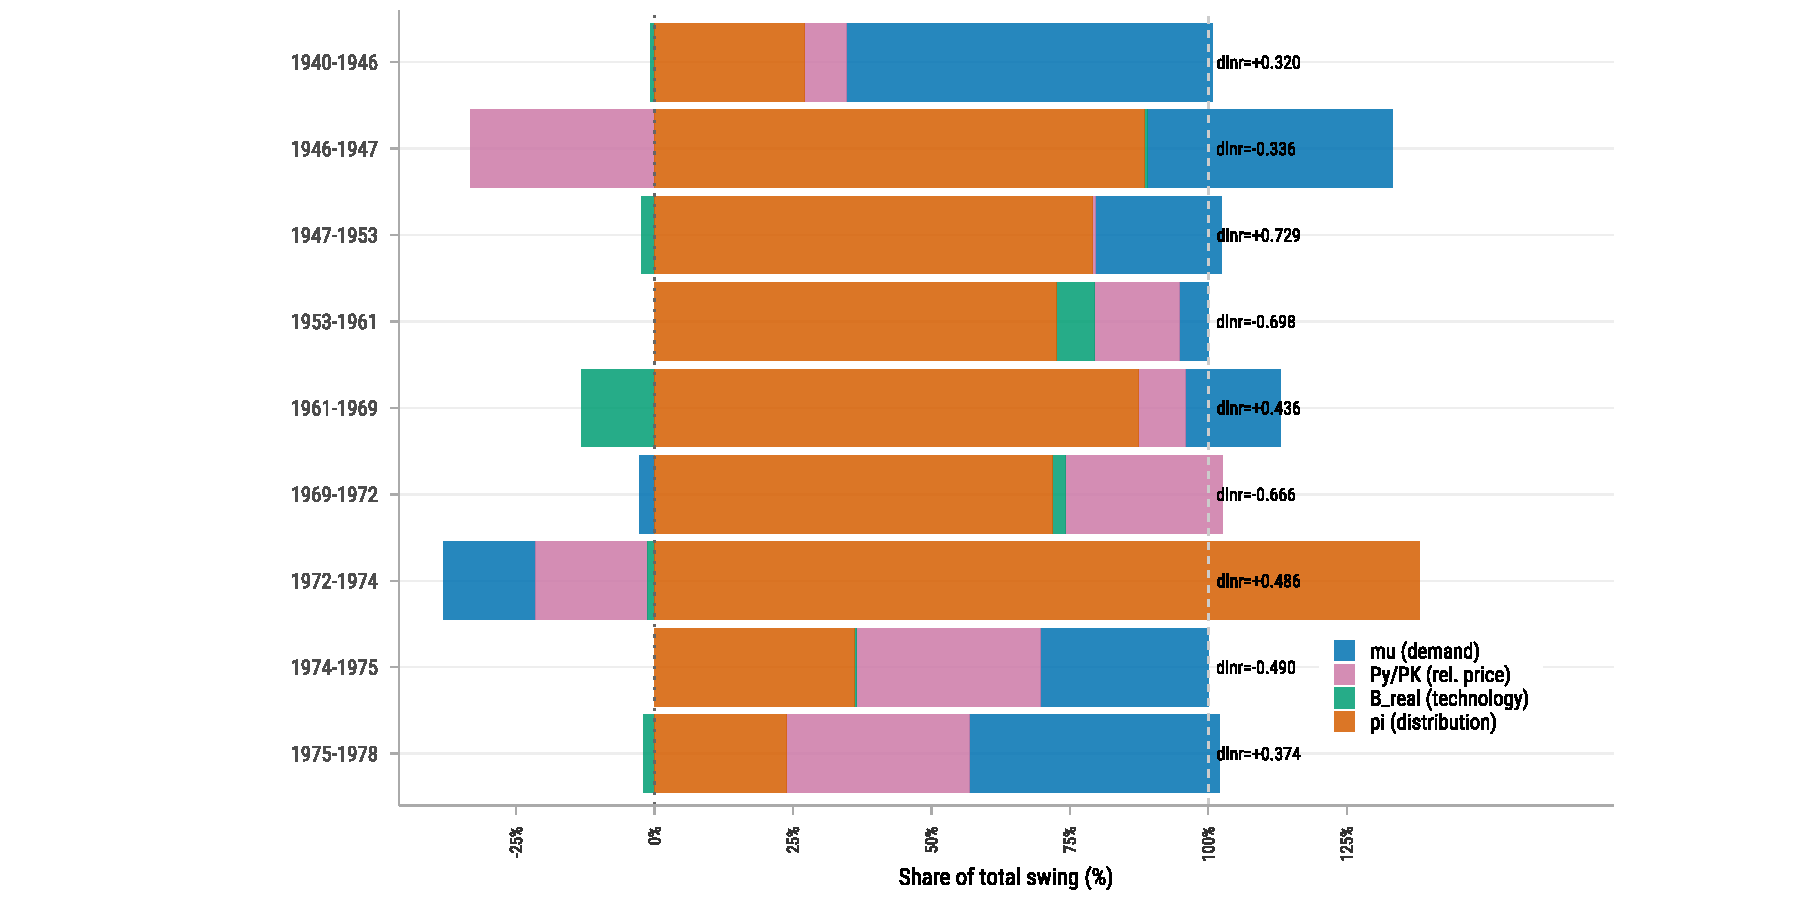
\includegraphics[width=\textwidth]{figures/fig_CL_B3_swing_composition}
\end{figure}

Traced across the ISI arc, the four-channel decomposition separates
what a three-channel framework cannot: the 1972--1974 expansion as a
distributional overdetermination episode unique to the political economy
of the Unidad Popular, and the 1974--1975 coup-period contraction as
the coincident action of demand destruction and capital-goods price
shock. What it cannot resolve is
the structural dynamic through which the BoP constraint converted
technological dependency into financial fragility --- the path-dependent
escalation from the mechanization trap to the debt trap that the
decomposition exposes but does not formalize. That is the object of
Chapter~3.

\section{Conclusion}
\label{ch2:sec:conclusion}

Fordism did not exhaust itself because any single mechanism failed.
It exhausted itself because the mechanisms that had sustained it
were structurally incompatible --- and the four-channel decomposition
makes this legible. By 1970, the US non-financial corporate profit
rate was under simultaneous pressure from distribution, demand, and
relational mechanization: the profit share eroded under
full-employment wage militancy; real capital productivity hit its
Taylorist ceiling as deskilling became a fetter rather than an
instrument of accumulation; and capacity utilization fell as fiscal
space for demand management contracted. No institutional lever was
capable of relieving more than one of these pressures at a time,
and the settlement that had counteracted them separately could not
contain them jointly.

The distribution-conditioned transformation elasticity recovered here
sits at $\hat{\theta}(\bar{\omega}) = 0.918$ --- structural
over-accumulation, operative throughout the Fordist period, with
capital accumulating faster than productive capacity expanded at the
wage shares the settlement sustained. The Fordist settlement managed
this tendency rather than resolving it: Taylorist compositional
upgrading held $B_r$ on an ascending path ($B_r$ rising from 58.6
to 63.5 across the Fordist transition) even as the transformation
elasticity kept the capacity frontier under downward pressure. When
the profitability decomposition is laid against this backdrop, the
1966--1970 contraction reads differently from every earlier episode
in the postwar record. The distribution, demand, and productivity
channels contracted simultaneously, with no offsetting force in any
of them --- 34.5\% distributional, 29.2\% real capital productivity,
29.8\% demand. The settlement had counteracted each pressure
separately through different institutional levers; it had no lever
capable of acting on all three at once. The 1972--1974 contraction,
by contrast, was primarily a price event: 57.8\% of the compounded
decline operated through $P_Y/P_K$ as the oil shock transmitted
through the relative capital goods price, while real productive
efficiency continued to improve ($B_r$ offset $-13.0\%$). What
separates these two episodes is not their magnitude but the structure
of their causation --- and under this reading, the asymmetry in the
productive efficiency channel is the evidence: $B_r$ deteriorated in
1966--1970 and improved in 1972--1974. The decomposition cannot
resolve the direction of the institutional causality: whether demand
activation counteracted over-accumulation, or whether over-accumulation
made demand activation structurally necessary. That is the question
Chapter~3 must address.

The Bretton Woods collapse couples the two crises but does not
symmetrize them. For the United States, the 1972--1974 world-market
stagnation tendency operated as a single-sided shock: capital goods
prices rose relative to output prices as energy-intensive production
costs transmitted through the capital goods deflator, compressing
$P_Y/P_K$ while real productive efficiency continued to improve.
For Chile, the same world monetary dislocation arrived as a
terms-of-trade scissors: copper prices collapsed as petrodollar
recycling restructured commodity markets, compressing export revenue;
simultaneously, the dollar float and import liberalization raised
the cost of machinery and equipment in domestic currency. The
four-channel decomposition is the instrument that separates these
two forms of the same world-monetary event. They share an external
origin --- the dissolution of the Bretton Woods architecture ---
but they operate through structurally different transmission
mechanisms in center and periphery, and conflating them would
obscure the relational structure that makes the coupling
analytically consequential.

The Chilean results illuminate what the US case, taken alone, cannot make visible: that the
structural configuration of peripheral capitalism under the
balance-of-payments constraint is analytically distinct from the
center, not a lagged or institutionally weaker version of it. The
distinction operates through relational mechanization.
$\hat{\theta}^{CL} < 1$ throughout the full ISI arc, indicating a
deeper over-accumulation tendency than the US, but the governing
mechanism is structural-dynamic rather than distributional. The
balance-of-payments constraint makes accumulation demand
self-undermining: higher $g_K$ raises the import bill for capital
goods whose domestic production the periphery cannot substitute
at scale ($\hat{\zeta}_1 = 0.930$; each unit of machinery
accumulation raises structural import demand by 0.930), draining
effective demand to capital-goods exporters and bounding the
$\hat{\mu}$ gains that ISI industrialization sought. This is not
a policy failure correctable by distributional adjustment. It is
the structural contradiction between the requirements of
capacity-building and the foreign-exchange constraint imposed by
technological dependency on capital-goods exporters --- a
contradiction that the Fordist settlement at the center did not
face because the US capital goods sector is domestically governed
and Bretton Woods capital controls insulated the domestic
accumulation dynamic from world-market price transmission.

The trap deepens path-dependently as industrialization advances.
Non-reinvested surplus flowing into luxury consumption imports
($\hat{\zeta}_2 = 0.445$) adds a surplus-drain channel beyond
the structural machinery requirement. The secular deterioration
of the capital-goods terms of trade --- output prices governed
by commodity cycles, capital goods prices by the productivity
of center exporters --- means the real cost of achieving any
given degree of mechanization rises as ISI deepens into higher
technological tiers, precisely as import substitution was
supposed to relax it. As each ISI tier approaches saturation,
the foreign exchange required per unit of capacity expansion
rises relative to what export revenues can generate. When the
Bretton Woods collapse accelerates the terms-of-trade scissors,
the latent technological trap converts into a financial crisis:
the balance-of-payments constraint shifts from a structural
brake on mechanization to an acute shadow-price activation that
compresses the feasible frontier directly (Regime~2:
$\hat{\alpha}_y^{R2} = -0.017$, a 5.5-fold deceleration in
frontier adjustment relative to Regime~1). The 1972--1974
distributional overdetermination ($s_\pi = 1.381$) is not the
cause of this transition; it is the political-military resolution
of a structural crisis that the economic mechanism could not
absorb internally.

The United States is therefore not a norm from which the Chilean
case deviates. It is the canonical study that makes the dynamics
of peripheral capitalism legible by contrast. The Fordist
settlement routinized demand activation ($\hat{\beta}_\mu =
+0.639$), absorbed distributional conflict through
productivity-indexed wages, and insulated domestic accumulation
from world-market dislocations through Bretton Woods capital
controls --- not because center capitalism resolved its structural
contradictions, but because it distributed them across multiple
institutional containment mechanisms that could offset each other.
The stability of the center was produced through conditions that
the periphery was structurally excluded --- the same world monetary
architecture that gave the US Fordist settlement its behavioral
demand signal made peripheral accumulation externally conditioned,
commodity-price dependent, and technologically bound to the
capital-goods sector of the center it could not substitute.
Understanding accumulation in peripheral capitalism is not an
exercise in area studies; it is the analysis of the relational
structure through which the conditions of center stability were
simultaneously the conditions of peripheral structural constraint.
Chapter~3 formalizes the law of motion through which that
constraint generates its own interruption --- the leverage ratio
trajectory of the peripheral economy, at the shadow of the rise
and fall of the American Empire, is where that formalization
begins.

%</ch2body>

%%%%%%%%%%%%%%%%%%%%%%%%%%%%%%%%%%%%%%%%%%%%%%%%%%%%%%%%%%%%%%
%%%%%%%%%%%%% References %%%%%%%%%%%%%%%%%%%%%%%%%%%%%%%%%%%%%
%%%%%%%%%%%%%%%%%%%%%%%%%%%%%%%%%%%%%%%%%%%%%%%%%%%%%%%%%%%%%%
% REF References
\pagebreak
\label{ch2:references}
\bibliographystyle{apalike}
\bibliography{../references}


\pagebreak
\appendix
%<*ch2appendix>
\section{Cost-Eficient Choice of Technique under Induced Mechanization}
\label{app:us_formal_id}
\input{appendix/appendix_theta_identification}

\pagebreak
\section{US Estimation of Capacity Utilization via MPF}
\label{app:us_stage_a}
%% ===========================================================================
%% APPENDIX A — US Stage A: Johansen Structural Identification
%% File: appendix_us_stage_a.tex
%% Input into main document via %% ===========================================================================
%% APPENDIX A — US Stage A: Johansen Structural Identification
%% File: appendix_us_stage_a.tex
%% Input into main document via %% ===========================================================================
%% APPENDIX A — US Stage A: Johansen Structural Identification
%% File: appendix_us_stage_a.tex
%% Input into main document via \input{appendix_us_stage_a}
%% All labels prefixed app: for appendix, sa: for Stage A
%% Cross-reference from §2.8.1 via \ref{} and \eqref{}
%% ===========================================================================

This appendix reports the full econometric detail underlying the US
mechanization possibility frontier (MPF) and capacity utilization estimates
presented in Section~\ref{sec:results_us}. All results are produced by
Johansen reduced-rank regression on the state vector
%
\begin{equation}
    X_t = \left(y_t,\; k_t,\; \omega_t,\; \omega_t k_t\right)'
    \label{eq:sa:state_vector}
\end{equation}
%
with a restricted constant (\texttt{ecdet="const"}, Case~3), where $y_t =
\ln(\text{GDP}_{real})$, $k_t = \ln(K^G_{NR,real})$ is the log of the gross
non-residential capital stock, and $\omega_t = EC_{NF}/GVA_{NF}$ is the
non-financial corporate wage share.\footnote{The wage share $\omega_t$ is the
distributional variable per the 2026-04-05 specification lock. Capital is
measured as the gross stock --- see Section~\ref{sec:data} for the capital
accounting rationale.}


% ---- A.1 Rank Determination ------------------------------------------------
\subsection{Rank Determination}
\label{app:sa:rank}

The Johansen trace test is conducted on the system~\eqref{eq:sa:state_vector}
with lag order $K=2$ and long-run normalization (\texttt{spec="longrun"}).
Table~\ref{tab:sa:trace} reports the first eigenvalue; the full trace
sequence is available on request.

\begin{table}[htbp]
\centering
\caption{Johansen Trace Test --- First Eigenvalue}
\label{tab:sa:trace}
\begin{threeparttable}
\begin{tabular}{lccc}
\toprule
$H_0$ & $\lambda_1$ & Trace statistic & 5\% CV \\
\midrule
$r \leq 0$ & $0.5901$ & $159.26$ & $53.12$ \\
\bottomrule
\end{tabular}
\begin{tablenotes}
\small
\item \textit{Notes:} Sample 1929--2024 ($T = 96$). $K = 2$ lags,
\texttt{spec="longrun"}, \texttt{ecdet="const"}.
Critical values from \citet{Osterwald-Lenum1992}.
The null $r \leq 0$ is rejected at any conventional level.
\end{tablenotes}
\end{threeparttable}
\end{table}

The first eigenvalue alone ($\lambda_1 = 0.590$) carries overwhelming
evidence of at least one cointegrating relation. The full system supports
$r = 3$ (see the rank sequence in the estimation script); we verify in
Appendix~\ref{app:sa:rank_invariance} that the first eigenvector is
invariant to the rank specification.


% ---- A.2 Cointegrating Vector (CV1) ----------------------------------------
\subsection{Cointegrating Vector}
\label{app:sa:cv1}

The $y$-normalized first eigenvector $\hat{\beta}_1$ is:
%
\begin{equation}
    y_t = \underbrace{8.924}_{\alpha_1}\, k_t
        + \underbrace{222.161}_{\gamma}\, \omega_t
        - \underbrace{12.851}_{\alpha_2}\, \omega_t k_t
        - 138.254
    \label{eq:sa:cv1}
\end{equation}
%
Table~\ref{tab:sa:cv1_params} reports the structural parameters.

\begin{table}[htbp]
\centering
\caption{MPF Structural Parameters (CV1, $y$-normalized)}
\label{tab:sa:cv1_params}
\begin{threeparttable}
\begin{tabular}{llr}
\toprule
Parameter & Structural role & Estimate \\
\midrule
$\alpha_1$ & Base elasticity ($\theta$ at $\omega = 0$) & $8.9238$ \\
$\alpha_2$ & Distribution slope ($\partial\theta / \partial\omega$) & $-12.8509$ \\
$\gamma$   & Direct distributional level shift & $222.1611$ \\
$c_1$      & Constant & $-138.2544$ \\
\bottomrule
\end{tabular}
\begin{tablenotes}
\small
\item \textit{Notes:} Estimated via Johansen MLE on the state
vector~\eqref{eq:sa:state_vector}. Coefficients are identical under
$r=1$ and $r=3$ (see Table~\ref{tab:sa:rank_invariance}).
\end{tablenotes}
\end{threeparttable}
\end{table}

The distribution-conditioned transformation elasticity is:
%
\begin{equation}
    \boxed{\hat{\theta}(\omega_t) = \alpha_1 - \alpha_2\,\omega_t
        = 8.924 - 12.851\,\omega_t}
    \label{eq:sa:theta_omega}
\end{equation}
%
This is the empirical counterpart of the theoretical object
$\theta(\Lambda)$ in the reproduction function
(Section~\ref{sec:analytical_framework}). The sign $\alpha_2 < 0$
satisfies the FOC-grounded restriction: higher wage share reduces the
capacity transformation elasticity.


% ---- A.3 Regime Partition ---------------------------------------------------
\subsection{Regime Partition}
\label{app:sa:regime}

Setting $\hat{\theta}(\omega) = 1$ in~\eqref{eq:sa:theta_omega} and solving:
%
\begin{equation}
    \omega_H = \frac{\alpha_1 - 1}{\alpha_2} = \frac{8.924 - 1}{12.851}
    = 0.617
    \label{eq:sa:omega_H}
\end{equation}
%
This is the Harrodian knife-edge: the wage share at which the frontier
grows at the same rate as the capital stock ($\hat{\theta} = 1$). Since
$\omega_H = 0.617$ lies inside the sample range
$[\omega_{\min}, \omega_{\max}] = [0.540, 0.682]$, the regime switching
between over-accumulation ($\hat{\theta} < 1$, frontier lags capital) and
under-accumulation of accumulation demand ($\hat{\theta} > 1$, frontier outpaces capital) is empirically operative.

The crisis boundary ($\hat{\theta} = 0$) obtains at:
%
\begin{equation}
    \omega^* = \frac{\alpha_1}{\alpha_2} = \frac{8.924}{12.851}
    = 0.694
    \label{eq:sa:omega_star}
\end{equation}
%
which lies outside the observed sample --- the economy never reaches the
structural collapse threshold.

Table~\ref{tab:sa:regime_summary} summarizes the regime partition.

\begin{table}[htbp]
\centering
\caption{Regime Partition of $\hat{\theta}(\omega_t)$}
\label{tab:sa:regime_summary}
\begin{threeparttable}
\begin{tabular}{lr}
\toprule
Object & Value \\
\midrule
$\hat{\theta}$ at $\bar{\omega} = 0.623$ & $0.921$ \\
$\hat{\theta}$ range $[\omega_{\min}, \omega_{\max}]$ & $[0.214,\; 1.666]$ \\
$\omega_H$ ($\hat{\theta} = 1$ knife-edge) & $0.617$ \\
$\omega^*$ ($\hat{\theta} = 0$ crisis boundary) & $0.694$ \\
\% sample under-accumulation ($\hat{\theta} > 1$) & 29\% \\
\% sample over-accumulation ($\hat{\theta} < 1$) & 71\% \\
\bottomrule
\end{tabular}
\begin{tablenotes}
\small
\item \textit{Notes:} Regime classification based on annual
$\hat{\theta}(\omega_t)$ from~\eqref{eq:sa:theta_omega}.
Sub-/super-Harrodian refers to whether the productive capacity frontier
grows slower/faster than the capital stock.
\end{tablenotes}
\end{threeparttable}
\end{table}


% ---- A.4 Error Correction Structure ----------------------------------------
\subsection{Error Correction Loading ($r=1$)}
\label{app:sa:alpha}

Table~\ref{tab:sa:alpha} reports the loading vector $\hat{\alpha}$ under
$r = 1$.

\begin{table}[htbp]
\centering
\caption{Loading Vector $\hat{\alpha}$ --- Rank 1}
\label{tab:sa:alpha}
\begin{threeparttable}
\begin{tabular}{lrrr}
\toprule
Equation & $\hat{\alpha}$ & SE & $t$-stat \\
\midrule
$\Delta y_t$              & $+0.011$ & $0.015$ & $0.74$ \\
$\Delta k_t$              & $+0.024$ & $0.008$ & $2.89$** \\
$\Delta \omega_t$         & $+0.009$ & $0.003$ & $3.11$** \\
$\Delta(\omega_t k_t)$    & $+0.131$ & $0.046$ & $2.86$** \\
\bottomrule
\end{tabular}
\begin{tablenotes}
\small
\item \textit{Notes:} Johansen MLE, $r = 1$.
** significant at 5\%. Output does not error-correct to the MPF
($t = 0.74$); capital and the wage share adjust. This pattern is
consistent with the theoretical architecture of
Section~\ref{sec:analytical_framework}: the MPF is a supply-side
locus, and output deviations from the frontier are
demand-determined.
\end{tablenotes}
\end{threeparttable}
\end{table}

% ---- A.6 Rank Invariance ---------------------------------------------------
\subsection{Rank Invariance: $r = 1$ versus $r = 3$}
\label{app:sa:rank_invariance}

A key property of Johansen's procedure is that eigenvectors are ordered by
eigenvalue magnitude. The first eigenvector $\hat{\beta}_1$ should therefore
be invariant to the rank specification. Table~\ref{tab:sa:rank_invariance}
confirms this.

\begin{table}[H]
\centering
\caption{First Eigenvector under $r = 1$ and $r = 3$}
\label{tab:sa:rank_invariance}
\begin{threeparttable}
\begin{tabular}{lrr}
\toprule
Parameter & $r = 1$ & $r = 3$ \\
\midrule
$\alpha_1$ ($k$)         & $8.9238$    & $8.9238$ \\
$\gamma$ ($\omega$)      & $222.1611$  & $222.1611$ \\
$\alpha_2$ ($\omega k$)  & $-12.8509$  & $-12.8509$ \\
$c_1$ (const)            & $-138.2544$ & $-138.2544$ \\
$\hat{\theta}(\bar{\omega})$ & $0.9206$ & $0.9206$ \\
\bottomrule
\end{tabular}
\begin{tablenotes}
\small
\item \textit{Notes:} Perfect numerical agreement. The MPF
identification does not depend on the additional cointegrating
relations. Additional rank adds error correction channels (ECT$_2$
disciplines distribution, ECT$_3$ is output-specific) but does not
alter the structural content of $\hat{\beta}_1$.
\end{tablenotes}
\end{threeparttable}
\end{table}


% ---- A.7 Restriction Tests -------------------------------------------------
\subsection{Over-Identification: Restriction Tests}
\label{app:sa:restrictions}

Two sets of restrictions are tested on the $r = 3$ system.

\paragraph{(i) Joint restriction $\omega = 0$, $\omega k = 1/2$.}
This restriction is \emph{accepted} across all three cointegrating vectors
(LR $= 0.00$, $p = 1.00$). Under the restriction, $\hat{\theta}$
collapses to a narrow over-accumulation band $[1.48, 1.54]$, eliminating
regime switching entirely. Since the theoretical framework requires
$\omega_H$ inside the sample (Section~\ref{sec:analytical_framework}),
the restricted specification is interpreted as supportive evidence to the assumption of a mechanization function with increasing returns at decreasing rates on labour productivity growth from mechanization intensity.

\paragraph{(ii) Test of $\alpha_1 = 1$ under the joint restriction.}
Rejected for CV2 and CV3 (LR $= 17.06$, $p = 0.0007$), confirming that
the base elasticity $\alpha_1$ is significantly greater than unity. This
result supports the wide-range specification reported in
Table~\ref{tab:sa:cv1_params}.


% ---- A.8 Capacity Utilization Construction ---------------------------------
\subsection{Capacity Utilization: Construction and Sensitivity}
\label{app:sa:mu_construction}

\subsubsection{Structural Closure}
\label{app:sa:mu_structural}

The capacity utilization rate $\hat{\mu}_t$ is constructed via a growth
closure. The frontier is pinned at:
%
\begin{equation}
    \hat{\mu}(1948) = 0.80
    \label{eq:sa:mu_pin}
\end{equation}
%
following the Federal Reserve benchmark. The growth rate of productive
capacity is:
%
\begin{equation}
    g_{Y^p_t} = \hat{\theta}(\omega_t) \cdot g_{K_t}
    \label{eq:sa:frontier_growth}
\end{equation}
%
and $Y^p_t$ is accumulated forward and backward from the pin year, yielding:
%
\begin{equation}
   \mu_t = \frac{Y_t}{Y^p_t}
    \label{eq:sa:mu_def}
\end{equation}

Table~\ref{tab:sa:mu_periods} reports period averages.

\begin{table}[htbp]
\centering
\caption{$\hat{\theta}$ and $\hat{\mu}$ Period Averages}
\label{tab:sa:mu_periods}
\begin{threeparttable}
\begin{tabular}{llrrr}
\toprule
Period & Years & $n$ & $\bar{\theta}$ & $\bar{\mu}$ \\
\midrule
Pre-Fordist  & 1929--1944 & 16 & $0.831$ & $0.780$ \\
Fordist      & 1945--1973 & 29 & $0.787$ & $0.734$ \\
Post-Fordist & 1974--2024 & 51 & $1.021$ & $0.681$ \\
\bottomrule
\end{tabular}
\begin{tablenotes}
\small
\item \textit{Notes:} $\hat{\theta}(\omega_t)$
from~\eqref{eq:sa:theta_omega}; $\hat{\mu}_t$
from~\eqref{eq:sa:mu_def} with pin~\eqref{eq:sa:mu_pin}. The
Post-Fordist under-accumulation mean ($\bar{\theta} > 1$) drives
the secular decline in $\hat{\mu}$: the frontier expansion outpaces the realized output. 
\end{tablenotes}
\end{threeparttable}
\end{table}

Key landmarks in the $\hat{\mu}_t$ series:
%
\begin{itemize}
    \item \textbf{1932--33}: $\hat{\mu} \approx 0.58$--$0.60$ (Great
        Depression trough --- severe underutilization).
    \item \textbf{1943--44}: $\hat{\mu} > 1.0$ (wartime full capacity ---
        the only years at or above the frontier).
    \item \textbf{1945--1973}: $\hat{\mu}$ stabilizes at $0.73$--$0.76$
        (Fordist plateau).
    \item \textbf{Post-2004}: $\hat{\mu}$ declines from $0.74$ to $0.55$
        (2024), as the super-Harrodian regime makes the frontier grow
        faster than actual output.
\end{itemize}

\subsubsection{ECT-Based Alternative}
\label{app:sa:mu_ect}

An alternative capacity utilization measure uses the full cointegrating
residual in the same fashion as \citet{Shaikh2016} does: 
%
\begin{equation}
    \hat{\mu}^{ect}_t = \exp\!\left(\text{ECT}_{1,t}
    - \overline{\text{ECT}_1}\right)
    \label{eq:sa:mu_ect}
\end{equation}
%
centered on 1 by construction. Period means: Pre-Fordist ($1.75$),
Fordist ($1.12$), Post-Fordist ($0.94$). This measure confirms the secular
decline but uses a different normalization and includes the direct $\omega$
and constant terms. $\hat{\mu}^{ect}_t$ serves as a robustness check;
the structural closure $\hat{\mu}_t$ from~\eqref{eq:sa:mu_def} is the
primary object for Stages~B and~C.


% ---- A.9 Label Directory ---------------------------------------------------
%
% CROSS-REFERENCE DIRECTORY for §2.8.1 drafting:
%
% EQUATIONS:
%   \eqref{eq:sa:state_vector}    — state vector definition
%   \eqref{eq:sa:cv1}             — cointegrating vector (MPF)
%   \eqref{eq:sa:theta_omega}     — theta(omega) structural formula
%   \eqref{eq:sa:omega_H}         — Harrodian knife-edge
%   \eqref{eq:sa:omega_star}      — crisis boundary
%   \eqref{eq:sa:ect1}            — ECT definition
%   \eqref{eq:sa:mu_pin}          — pin year condition
%   \eqref{eq:sa:frontier_growth} — frontier growth closure
%   \eqref{eq:sa:mu_def}          — mu definition
%   \eqref{eq:sa:mu_ect}          — ECT-based mu (robustness)
%
% TABLES:
%   \ref{tab:sa:trace}            — trace test
%   \ref{tab:sa:cv1_params}       — MPF structural parameters
%   \ref{tab:sa:regime_summary}   — regime partition
%   \ref{tab:sa:alpha}            — loading vector (r=1)
%   \ref{tab:sa:ect_adf}          — ECT stationarity
%   \ref{tab:sa:rank_invariance}  — rank invariance (r=1 vs r=3)
%   \ref{tab:sa:mu_periods}       — theta and mu period averages
%
% SECTIONS:
%   \ref{app:us_stage_a}          — appendix top-level
%   \ref{app:sa:rank}             — rank determination
%   \ref{app:sa:cv1}              — cointegrating vector
%   \ref{app:sa:regime}           — regime partition
%   \ref{app:sa:alpha}            — error correction loading
%   \ref{app:sa:ect_stationarity} — ECT stationarity
%   \ref{app:sa:rank_invariance}  — rank invariance
%   \ref{app:sa:restrictions}     — restriction tests
%   \ref{app:sa:mu_construction}  — mu construction
%   \ref{app:sa:mu_structural}    — structural closure
%   \ref{app:sa:mu_ect}           — ECT-based mu
%   \ref{app:sa:pin_sensitivity}  — pin-year sensitivity (deferred)
%
% FORWARD REFERENCES (must exist in main body):
%   \ref{sec:results_us}          — §2.8.1 US results
%   \ref{sec:analytical_framework}— §2.3 analytical framework
%   \ref{sec:data}                — §2.4 data section
%

%% All labels prefixed app: for appendix, sa: for Stage A
%% Cross-reference from §2.8.1 via \ref{} and \eqref{}
%% ===========================================================================

This appendix reports the full econometric detail underlying the US
mechanization possibility frontier (MPF) and capacity utilization estimates
presented in Section~\ref{sec:results_us}. All results are produced by
Johansen reduced-rank regression on the state vector
%
\begin{equation}
    X_t = \left(y_t,\; k_t,\; \omega_t,\; \omega_t k_t\right)'
    \label{eq:sa:state_vector}
\end{equation}
%
with a restricted constant (\texttt{ecdet="const"}, Case~3), where $y_t =
\ln(\text{GDP}_{real})$, $k_t = \ln(K^G_{NR,real})$ is the log of the gross
non-residential capital stock, and $\omega_t = EC_{NF}/GVA_{NF}$ is the
non-financial corporate wage share.\footnote{The wage share $\omega_t$ is the
distributional variable per the 2026-04-05 specification lock. Capital is
measured as the gross stock --- see Section~\ref{sec:data} for the capital
accounting rationale.}


% ---- A.1 Rank Determination ------------------------------------------------
\subsection{Rank Determination}
\label{app:sa:rank}

The Johansen trace test is conducted on the system~\eqref{eq:sa:state_vector}
with lag order $K=2$ and long-run normalization (\texttt{spec="longrun"}).
Table~\ref{tab:sa:trace} reports the first eigenvalue; the full trace
sequence is available on request.

\begin{table}[htbp]
\centering
\caption{Johansen Trace Test --- First Eigenvalue}
\label{tab:sa:trace}
\begin{threeparttable}
\begin{tabular}{lccc}
\toprule
$H_0$ & $\lambda_1$ & Trace statistic & 5\% CV \\
\midrule
$r \leq 0$ & $0.5901$ & $159.26$ & $53.12$ \\
\bottomrule
\end{tabular}
\begin{tablenotes}
\small
\item \textit{Notes:} Sample 1929--2024 ($T = 96$). $K = 2$ lags,
\texttt{spec="longrun"}, \texttt{ecdet="const"}.
Critical values from \citet{Osterwald-Lenum1992}.
The null $r \leq 0$ is rejected at any conventional level.
\end{tablenotes}
\end{threeparttable}
\end{table}

The first eigenvalue alone ($\lambda_1 = 0.590$) carries overwhelming
evidence of at least one cointegrating relation. The full system supports
$r = 3$ (see the rank sequence in the estimation script); we verify in
Appendix~\ref{app:sa:rank_invariance} that the first eigenvector is
invariant to the rank specification.


% ---- A.2 Cointegrating Vector (CV1) ----------------------------------------
\subsection{Cointegrating Vector}
\label{app:sa:cv1}

The $y$-normalized first eigenvector $\hat{\beta}_1$ is:
%
\begin{equation}
    y_t = \underbrace{8.924}_{\alpha_1}\, k_t
        + \underbrace{222.161}_{\gamma}\, \omega_t
        - \underbrace{12.851}_{\alpha_2}\, \omega_t k_t
        - 138.254
    \label{eq:sa:cv1}
\end{equation}
%
Table~\ref{tab:sa:cv1_params} reports the structural parameters.

\begin{table}[htbp]
\centering
\caption{MPF Structural Parameters (CV1, $y$-normalized)}
\label{tab:sa:cv1_params}
\begin{threeparttable}
\begin{tabular}{llr}
\toprule
Parameter & Structural role & Estimate \\
\midrule
$\alpha_1$ & Base elasticity ($\theta$ at $\omega = 0$) & $8.9238$ \\
$\alpha_2$ & Distribution slope ($\partial\theta / \partial\omega$) & $-12.8509$ \\
$\gamma$   & Direct distributional level shift & $222.1611$ \\
$c_1$      & Constant & $-138.2544$ \\
\bottomrule
\end{tabular}
\begin{tablenotes}
\small
\item \textit{Notes:} Estimated via Johansen MLE on the state
vector~\eqref{eq:sa:state_vector}. Coefficients are identical under
$r=1$ and $r=3$ (see Table~\ref{tab:sa:rank_invariance}).
\end{tablenotes}
\end{threeparttable}
\end{table}

The distribution-conditioned transformation elasticity is:
%
\begin{equation}
    \boxed{\hat{\theta}(\omega_t) = \alpha_1 - \alpha_2\,\omega_t
        = 8.924 - 12.851\,\omega_t}
    \label{eq:sa:theta_omega}
\end{equation}
%
This is the empirical counterpart of the theoretical object
$\theta(\Lambda)$ in the reproduction function
(Section~\ref{sec:analytical_framework}). The sign $\alpha_2 < 0$
satisfies the FOC-grounded restriction: higher wage share reduces the
capacity transformation elasticity.


% ---- A.3 Regime Partition ---------------------------------------------------
\subsection{Regime Partition}
\label{app:sa:regime}

Setting $\hat{\theta}(\omega) = 1$ in~\eqref{eq:sa:theta_omega} and solving:
%
\begin{equation}
    \omega_H = \frac{\alpha_1 - 1}{\alpha_2} = \frac{8.924 - 1}{12.851}
    = 0.617
    \label{eq:sa:omega_H}
\end{equation}
%
This is the Harrodian knife-edge: the wage share at which the frontier
grows at the same rate as the capital stock ($\hat{\theta} = 1$). Since
$\omega_H = 0.617$ lies inside the sample range
$[\omega_{\min}, \omega_{\max}] = [0.540, 0.682]$, the regime switching
between over-accumulation ($\hat{\theta} < 1$, frontier lags capital) and
under-accumulation of accumulation demand ($\hat{\theta} > 1$, frontier outpaces capital) is empirically operative.

The crisis boundary ($\hat{\theta} = 0$) obtains at:
%
\begin{equation}
    \omega^* = \frac{\alpha_1}{\alpha_2} = \frac{8.924}{12.851}
    = 0.694
    \label{eq:sa:omega_star}
\end{equation}
%
which lies outside the observed sample --- the economy never reaches the
structural collapse threshold.

Table~\ref{tab:sa:regime_summary} summarizes the regime partition.

\begin{table}[htbp]
\centering
\caption{Regime Partition of $\hat{\theta}(\omega_t)$}
\label{tab:sa:regime_summary}
\begin{threeparttable}
\begin{tabular}{lr}
\toprule
Object & Value \\
\midrule
$\hat{\theta}$ at $\bar{\omega} = 0.623$ & $0.921$ \\
$\hat{\theta}$ range $[\omega_{\min}, \omega_{\max}]$ & $[0.214,\; 1.666]$ \\
$\omega_H$ ($\hat{\theta} = 1$ knife-edge) & $0.617$ \\
$\omega^*$ ($\hat{\theta} = 0$ crisis boundary) & $0.694$ \\
\% sample under-accumulation ($\hat{\theta} > 1$) & 29\% \\
\% sample over-accumulation ($\hat{\theta} < 1$) & 71\% \\
\bottomrule
\end{tabular}
\begin{tablenotes}
\small
\item \textit{Notes:} Regime classification based on annual
$\hat{\theta}(\omega_t)$ from~\eqref{eq:sa:theta_omega}.
Sub-/super-Harrodian refers to whether the productive capacity frontier
grows slower/faster than the capital stock.
\end{tablenotes}
\end{threeparttable}
\end{table}


% ---- A.4 Error Correction Structure ----------------------------------------
\subsection{Error Correction Loading ($r=1$)}
\label{app:sa:alpha}

Table~\ref{tab:sa:alpha} reports the loading vector $\hat{\alpha}$ under
$r = 1$.

\begin{table}[htbp]
\centering
\caption{Loading Vector $\hat{\alpha}$ --- Rank 1}
\label{tab:sa:alpha}
\begin{threeparttable}
\begin{tabular}{lrrr}
\toprule
Equation & $\hat{\alpha}$ & SE & $t$-stat \\
\midrule
$\Delta y_t$              & $+0.011$ & $0.015$ & $0.74$ \\
$\Delta k_t$              & $+0.024$ & $0.008$ & $2.89$** \\
$\Delta \omega_t$         & $+0.009$ & $0.003$ & $3.11$** \\
$\Delta(\omega_t k_t)$    & $+0.131$ & $0.046$ & $2.86$** \\
\bottomrule
\end{tabular}
\begin{tablenotes}
\small
\item \textit{Notes:} Johansen MLE, $r = 1$.
** significant at 5\%. Output does not error-correct to the MPF
($t = 0.74$); capital and the wage share adjust. This pattern is
consistent with the theoretical architecture of
Section~\ref{sec:analytical_framework}: the MPF is a supply-side
locus, and output deviations from the frontier are
demand-determined.
\end{tablenotes}
\end{threeparttable}
\end{table}

% ---- A.6 Rank Invariance ---------------------------------------------------
\subsection{Rank Invariance: $r = 1$ versus $r = 3$}
\label{app:sa:rank_invariance}

A key property of Johansen's procedure is that eigenvectors are ordered by
eigenvalue magnitude. The first eigenvector $\hat{\beta}_1$ should therefore
be invariant to the rank specification. Table~\ref{tab:sa:rank_invariance}
confirms this.

\begin{table}[H]
\centering
\caption{First Eigenvector under $r = 1$ and $r = 3$}
\label{tab:sa:rank_invariance}
\begin{threeparttable}
\begin{tabular}{lrr}
\toprule
Parameter & $r = 1$ & $r = 3$ \\
\midrule
$\alpha_1$ ($k$)         & $8.9238$    & $8.9238$ \\
$\gamma$ ($\omega$)      & $222.1611$  & $222.1611$ \\
$\alpha_2$ ($\omega k$)  & $-12.8509$  & $-12.8509$ \\
$c_1$ (const)            & $-138.2544$ & $-138.2544$ \\
$\hat{\theta}(\bar{\omega})$ & $0.9206$ & $0.9206$ \\
\bottomrule
\end{tabular}
\begin{tablenotes}
\small
\item \textit{Notes:} Perfect numerical agreement. The MPF
identification does not depend on the additional cointegrating
relations. Additional rank adds error correction channels (ECT$_2$
disciplines distribution, ECT$_3$ is output-specific) but does not
alter the structural content of $\hat{\beta}_1$.
\end{tablenotes}
\end{threeparttable}
\end{table}


% ---- A.7 Restriction Tests -------------------------------------------------
\subsection{Over-Identification: Restriction Tests}
\label{app:sa:restrictions}

Two sets of restrictions are tested on the $r = 3$ system.

\paragraph{(i) Joint restriction $\omega = 0$, $\omega k = 1/2$.}
This restriction is \emph{accepted} across all three cointegrating vectors
(LR $= 0.00$, $p = 1.00$). Under the restriction, $\hat{\theta}$
collapses to a narrow over-accumulation band $[1.48, 1.54]$, eliminating
regime switching entirely. Since the theoretical framework requires
$\omega_H$ inside the sample (Section~\ref{sec:analytical_framework}),
the restricted specification is interpreted as supportive evidence to the assumption of a mechanization function with increasing returns at decreasing rates on labour productivity growth from mechanization intensity.

\paragraph{(ii) Test of $\alpha_1 = 1$ under the joint restriction.}
Rejected for CV2 and CV3 (LR $= 17.06$, $p = 0.0007$), confirming that
the base elasticity $\alpha_1$ is significantly greater than unity. This
result supports the wide-range specification reported in
Table~\ref{tab:sa:cv1_params}.


% ---- A.8 Capacity Utilization Construction ---------------------------------
\subsection{Capacity Utilization: Construction and Sensitivity}
\label{app:sa:mu_construction}

\subsubsection{Structural Closure}
\label{app:sa:mu_structural}

The capacity utilization rate $\hat{\mu}_t$ is constructed via a growth
closure. The frontier is pinned at:
%
\begin{equation}
    \hat{\mu}(1948) = 0.80
    \label{eq:sa:mu_pin}
\end{equation}
%
following the Federal Reserve benchmark. The growth rate of productive
capacity is:
%
\begin{equation}
    g_{Y^p_t} = \hat{\theta}(\omega_t) \cdot g_{K_t}
    \label{eq:sa:frontier_growth}
\end{equation}
%
and $Y^p_t$ is accumulated forward and backward from the pin year, yielding:
%
\begin{equation}
   \mu_t = \frac{Y_t}{Y^p_t}
    \label{eq:sa:mu_def}
\end{equation}

Table~\ref{tab:sa:mu_periods} reports period averages.

\begin{table}[htbp]
\centering
\caption{$\hat{\theta}$ and $\hat{\mu}$ Period Averages}
\label{tab:sa:mu_periods}
\begin{threeparttable}
\begin{tabular}{llrrr}
\toprule
Period & Years & $n$ & $\bar{\theta}$ & $\bar{\mu}$ \\
\midrule
Pre-Fordist  & 1929--1944 & 16 & $0.831$ & $0.780$ \\
Fordist      & 1945--1973 & 29 & $0.787$ & $0.734$ \\
Post-Fordist & 1974--2024 & 51 & $1.021$ & $0.681$ \\
\bottomrule
\end{tabular}
\begin{tablenotes}
\small
\item \textit{Notes:} $\hat{\theta}(\omega_t)$
from~\eqref{eq:sa:theta_omega}; $\hat{\mu}_t$
from~\eqref{eq:sa:mu_def} with pin~\eqref{eq:sa:mu_pin}. The
Post-Fordist under-accumulation mean ($\bar{\theta} > 1$) drives
the secular decline in $\hat{\mu}$: the frontier expansion outpaces the realized output. 
\end{tablenotes}
\end{threeparttable}
\end{table}

Key landmarks in the $\hat{\mu}_t$ series:
%
\begin{itemize}
    \item \textbf{1932--33}: $\hat{\mu} \approx 0.58$--$0.60$ (Great
        Depression trough --- severe underutilization).
    \item \textbf{1943--44}: $\hat{\mu} > 1.0$ (wartime full capacity ---
        the only years at or above the frontier).
    \item \textbf{1945--1973}: $\hat{\mu}$ stabilizes at $0.73$--$0.76$
        (Fordist plateau).
    \item \textbf{Post-2004}: $\hat{\mu}$ declines from $0.74$ to $0.55$
        (2024), as the super-Harrodian regime makes the frontier grow
        faster than actual output.
\end{itemize}

\subsubsection{ECT-Based Alternative}
\label{app:sa:mu_ect}

An alternative capacity utilization measure uses the full cointegrating
residual in the same fashion as \citet{Shaikh2016} does: 
%
\begin{equation}
    \hat{\mu}^{ect}_t = \exp\!\left(\text{ECT}_{1,t}
    - \overline{\text{ECT}_1}\right)
    \label{eq:sa:mu_ect}
\end{equation}
%
centered on 1 by construction. Period means: Pre-Fordist ($1.75$),
Fordist ($1.12$), Post-Fordist ($0.94$). This measure confirms the secular
decline but uses a different normalization and includes the direct $\omega$
and constant terms. $\hat{\mu}^{ect}_t$ serves as a robustness check;
the structural closure $\hat{\mu}_t$ from~\eqref{eq:sa:mu_def} is the
primary object for Stages~B and~C.


% ---- A.9 Label Directory ---------------------------------------------------
%
% CROSS-REFERENCE DIRECTORY for §2.8.1 drafting:
%
% EQUATIONS:
%   \eqref{eq:sa:state_vector}    — state vector definition
%   \eqref{eq:sa:cv1}             — cointegrating vector (MPF)
%   \eqref{eq:sa:theta_omega}     — theta(omega) structural formula
%   \eqref{eq:sa:omega_H}         — Harrodian knife-edge
%   \eqref{eq:sa:omega_star}      — crisis boundary
%   \eqref{eq:sa:ect1}            — ECT definition
%   \eqref{eq:sa:mu_pin}          — pin year condition
%   \eqref{eq:sa:frontier_growth} — frontier growth closure
%   \eqref{eq:sa:mu_def}          — mu definition
%   \eqref{eq:sa:mu_ect}          — ECT-based mu (robustness)
%
% TABLES:
%   \ref{tab:sa:trace}            — trace test
%   \ref{tab:sa:cv1_params}       — MPF structural parameters
%   \ref{tab:sa:regime_summary}   — regime partition
%   \ref{tab:sa:alpha}            — loading vector (r=1)
%   \ref{tab:sa:ect_adf}          — ECT stationarity
%   \ref{tab:sa:rank_invariance}  — rank invariance (r=1 vs r=3)
%   \ref{tab:sa:mu_periods}       — theta and mu period averages
%
% SECTIONS:
%   \ref{app:us_stage_a}          — appendix top-level
%   \ref{app:sa:rank}             — rank determination
%   \ref{app:sa:cv1}              — cointegrating vector
%   \ref{app:sa:regime}           — regime partition
%   \ref{app:sa:alpha}            — error correction loading
%   \ref{app:sa:ect_stationarity} — ECT stationarity
%   \ref{app:sa:rank_invariance}  — rank invariance
%   \ref{app:sa:restrictions}     — restriction tests
%   \ref{app:sa:mu_construction}  — mu construction
%   \ref{app:sa:mu_structural}    — structural closure
%   \ref{app:sa:mu_ect}           — ECT-based mu
%   \ref{app:sa:pin_sensitivity}  — pin-year sensitivity (deferred)
%
% FORWARD REFERENCES (must exist in main body):
%   \ref{sec:results_us}          — §2.8.1 US results
%   \ref{sec:analytical_framework}— §2.3 analytical framework
%   \ref{sec:data}                — §2.4 data section
%

%% All labels prefixed app: for appendix, sa: for Stage A
%% Cross-reference from §2.8.1 via \ref{} and \eqref{}
%% ===========================================================================

This appendix reports the full econometric detail underlying the US
mechanization possibility frontier (MPF) and capacity utilization estimates
presented in Section~\ref{sec:results_us}. All results are produced by
Johansen reduced-rank regression on the state vector
%
\begin{equation}
    X_t = \left(y_t,\; k_t,\; \omega_t,\; \omega_t k_t\right)'
    \label{eq:sa:state_vector}
\end{equation}
%
with a restricted constant (\texttt{ecdet="const"}, Case~3), where $y_t =
\ln(\text{GDP}_{real})$, $k_t = \ln(K^G_{NR,real})$ is the log of the gross
non-residential capital stock, and $\omega_t = EC_{NF}/GVA_{NF}$ is the
non-financial corporate wage share.\footnote{The wage share $\omega_t$ is the
distributional variable per the 2026-04-05 specification lock. Capital is
measured as the gross stock --- see Section~\ref{sec:data} for the capital
accounting rationale.}


% ---- A.1 Rank Determination ------------------------------------------------
\subsection{Rank Determination}
\label{app:sa:rank}

The Johansen trace test is conducted on the system~\eqref{eq:sa:state_vector}
with lag order $K=2$ and long-run normalization (\texttt{spec="longrun"}).
Table~\ref{tab:sa:trace} reports the first eigenvalue; the full trace
sequence is available on request.

\begin{table}[htbp]
\centering
\caption{Johansen Trace Test --- First Eigenvalue}
\label{tab:sa:trace}
\begin{threeparttable}
\begin{tabular}{lccc}
\toprule
$H_0$ & $\lambda_1$ & Trace statistic & 5\% CV \\
\midrule
$r \leq 0$ & $0.5901$ & $159.26$ & $53.12$ \\
\bottomrule
\end{tabular}
\begin{tablenotes}
\small
\item \textit{Notes:} Sample 1929--2024 ($T = 96$). $K = 2$ lags,
\texttt{spec="longrun"}, \texttt{ecdet="const"}.
Critical values from \citet{Osterwald-Lenum1992}.
The null $r \leq 0$ is rejected at any conventional level.
\end{tablenotes}
\end{threeparttable}
\end{table}

The first eigenvalue alone ($\lambda_1 = 0.590$) carries overwhelming
evidence of at least one cointegrating relation. The full system supports
$r = 3$ (see the rank sequence in the estimation script); we verify in
Appendix~\ref{app:sa:rank_invariance} that the first eigenvector is
invariant to the rank specification.


% ---- A.2 Cointegrating Vector (CV1) ----------------------------------------
\subsection{Cointegrating Vector}
\label{app:sa:cv1}

The $y$-normalized first eigenvector $\hat{\beta}_1$ is:
%
\begin{equation}
    y_t = \underbrace{8.924}_{\alpha_1}\, k_t
        + \underbrace{222.161}_{\gamma}\, \omega_t
        - \underbrace{12.851}_{\alpha_2}\, \omega_t k_t
        - 138.254
    \label{eq:sa:cv1}
\end{equation}
%
Table~\ref{tab:sa:cv1_params} reports the structural parameters.

\begin{table}[htbp]
\centering
\caption{MPF Structural Parameters (CV1, $y$-normalized)}
\label{tab:sa:cv1_params}
\begin{threeparttable}
\begin{tabular}{llr}
\toprule
Parameter & Structural role & Estimate \\
\midrule
$\alpha_1$ & Base elasticity ($\theta$ at $\omega = 0$) & $8.9238$ \\
$\alpha_2$ & Distribution slope ($\partial\theta / \partial\omega$) & $-12.8509$ \\
$\gamma$   & Direct distributional level shift & $222.1611$ \\
$c_1$      & Constant & $-138.2544$ \\
\bottomrule
\end{tabular}
\begin{tablenotes}
\small
\item \textit{Notes:} Estimated via Johansen MLE on the state
vector~\eqref{eq:sa:state_vector}. Coefficients are identical under
$r=1$ and $r=3$ (see Table~\ref{tab:sa:rank_invariance}).
\end{tablenotes}
\end{threeparttable}
\end{table}

The distribution-conditioned transformation elasticity is:
%
\begin{equation}
    \boxed{\hat{\theta}(\omega_t) = \alpha_1 - \alpha_2\,\omega_t
        = 8.924 - 12.851\,\omega_t}
    \label{eq:sa:theta_omega}
\end{equation}
%
This is the empirical counterpart of the theoretical object
$\theta(\Lambda)$ in the reproduction function
(Section~\ref{sec:analytical_framework}). The sign $\alpha_2 < 0$
satisfies the FOC-grounded restriction: higher wage share reduces the
capacity transformation elasticity.


% ---- A.3 Regime Partition ---------------------------------------------------
\subsection{Regime Partition}
\label{app:sa:regime}

Setting $\hat{\theta}(\omega) = 1$ in~\eqref{eq:sa:theta_omega} and solving:
%
\begin{equation}
    \omega_H = \frac{\alpha_1 - 1}{\alpha_2} = \frac{8.924 - 1}{12.851}
    = 0.617
    \label{eq:sa:omega_H}
\end{equation}
%
This is the Harrodian knife-edge: the wage share at which the frontier
grows at the same rate as the capital stock ($\hat{\theta} = 1$). Since
$\omega_H = 0.617$ lies inside the sample range
$[\omega_{\min}, \omega_{\max}] = [0.540, 0.682]$, the regime switching
between over-accumulation ($\hat{\theta} < 1$, frontier lags capital) and
under-accumulation of accumulation demand ($\hat{\theta} > 1$, frontier outpaces capital) is empirically operative.

The crisis boundary ($\hat{\theta} = 0$) obtains at:
%
\begin{equation}
    \omega^* = \frac{\alpha_1}{\alpha_2} = \frac{8.924}{12.851}
    = 0.694
    \label{eq:sa:omega_star}
\end{equation}
%
which lies outside the observed sample --- the economy never reaches the
structural collapse threshold.

Table~\ref{tab:sa:regime_summary} summarizes the regime partition.

\begin{table}[htbp]
\centering
\caption{Regime Partition of $\hat{\theta}(\omega_t)$}
\label{tab:sa:regime_summary}
\begin{threeparttable}
\begin{tabular}{lr}
\toprule
Object & Value \\
\midrule
$\hat{\theta}$ at $\bar{\omega} = 0.623$ & $0.921$ \\
$\hat{\theta}$ range $[\omega_{\min}, \omega_{\max}]$ & $[0.214,\; 1.666]$ \\
$\omega_H$ ($\hat{\theta} = 1$ knife-edge) & $0.617$ \\
$\omega^*$ ($\hat{\theta} = 0$ crisis boundary) & $0.694$ \\
\% sample under-accumulation ($\hat{\theta} > 1$) & 29\% \\
\% sample over-accumulation ($\hat{\theta} < 1$) & 71\% \\
\bottomrule
\end{tabular}
\begin{tablenotes}
\small
\item \textit{Notes:} Regime classification based on annual
$\hat{\theta}(\omega_t)$ from~\eqref{eq:sa:theta_omega}.
Sub-/super-Harrodian refers to whether the productive capacity frontier
grows slower/faster than the capital stock.
\end{tablenotes}
\end{threeparttable}
\end{table}


% ---- A.4 Error Correction Structure ----------------------------------------
\subsection{Error Correction Loading ($r=1$)}
\label{app:sa:alpha}

Table~\ref{tab:sa:alpha} reports the loading vector $\hat{\alpha}$ under
$r = 1$.

\begin{table}[htbp]
\centering
\caption{Loading Vector $\hat{\alpha}$ --- Rank 1}
\label{tab:sa:alpha}
\begin{threeparttable}
\begin{tabular}{lrrr}
\toprule
Equation & $\hat{\alpha}$ & SE & $t$-stat \\
\midrule
$\Delta y_t$              & $+0.011$ & $0.015$ & $0.74$ \\
$\Delta k_t$              & $+0.024$ & $0.008$ & $2.89$** \\
$\Delta \omega_t$         & $+0.009$ & $0.003$ & $3.11$** \\
$\Delta(\omega_t k_t)$    & $+0.131$ & $0.046$ & $2.86$** \\
\bottomrule
\end{tabular}
\begin{tablenotes}
\small
\item \textit{Notes:} Johansen MLE, $r = 1$.
** significant at 5\%. Output does not error-correct to the MPF
($t = 0.74$); capital and the wage share adjust. This pattern is
consistent with the theoretical architecture of
Section~\ref{sec:analytical_framework}: the MPF is a supply-side
locus, and output deviations from the frontier are
demand-determined.
\end{tablenotes}
\end{threeparttable}
\end{table}

% ---- A.6 Rank Invariance ---------------------------------------------------
\subsection{Rank Invariance: $r = 1$ versus $r = 3$}
\label{app:sa:rank_invariance}

A key property of Johansen's procedure is that eigenvectors are ordered by
eigenvalue magnitude. The first eigenvector $\hat{\beta}_1$ should therefore
be invariant to the rank specification. Table~\ref{tab:sa:rank_invariance}
confirms this.

\begin{table}[H]
\centering
\caption{First Eigenvector under $r = 1$ and $r = 3$}
\label{tab:sa:rank_invariance}
\begin{threeparttable}
\begin{tabular}{lrr}
\toprule
Parameter & $r = 1$ & $r = 3$ \\
\midrule
$\alpha_1$ ($k$)         & $8.9238$    & $8.9238$ \\
$\gamma$ ($\omega$)      & $222.1611$  & $222.1611$ \\
$\alpha_2$ ($\omega k$)  & $-12.8509$  & $-12.8509$ \\
$c_1$ (const)            & $-138.2544$ & $-138.2544$ \\
$\hat{\theta}(\bar{\omega})$ & $0.9206$ & $0.9206$ \\
\bottomrule
\end{tabular}
\begin{tablenotes}
\small
\item \textit{Notes:} Perfect numerical agreement. The MPF
identification does not depend on the additional cointegrating
relations. Additional rank adds error correction channels (ECT$_2$
disciplines distribution, ECT$_3$ is output-specific) but does not
alter the structural content of $\hat{\beta}_1$.
\end{tablenotes}
\end{threeparttable}
\end{table}


% ---- A.7 Restriction Tests -------------------------------------------------
\subsection{Over-Identification: Restriction Tests}
\label{app:sa:restrictions}

Two sets of restrictions are tested on the $r = 3$ system.

\paragraph{(i) Joint restriction $\omega = 0$, $\omega k = 1/2$.}
This restriction is \emph{accepted} across all three cointegrating vectors
(LR $= 0.00$, $p = 1.00$). Under the restriction, $\hat{\theta}$
collapses to a narrow over-accumulation band $[1.48, 1.54]$, eliminating
regime switching entirely. Since the theoretical framework requires
$\omega_H$ inside the sample (Section~\ref{sec:analytical_framework}),
the restricted specification is interpreted as supportive evidence to the assumption of a mechanization function with increasing returns at decreasing rates on labour productivity growth from mechanization intensity.

\paragraph{(ii) Test of $\alpha_1 = 1$ under the joint restriction.}
Rejected for CV2 and CV3 (LR $= 17.06$, $p = 0.0007$), confirming that
the base elasticity $\alpha_1$ is significantly greater than unity. This
result supports the wide-range specification reported in
Table~\ref{tab:sa:cv1_params}.


% ---- A.8 Capacity Utilization Construction ---------------------------------
\subsection{Capacity Utilization: Construction and Sensitivity}
\label{app:sa:mu_construction}

\subsubsection{Structural Closure}
\label{app:sa:mu_structural}

The capacity utilization rate $\hat{\mu}_t$ is constructed via a growth
closure. The frontier is pinned at:
%
\begin{equation}
    \hat{\mu}(1948) = 0.80
    \label{eq:sa:mu_pin}
\end{equation}
%
following the Federal Reserve benchmark. The growth rate of productive
capacity is:
%
\begin{equation}
    g_{Y^p_t} = \hat{\theta}(\omega_t) \cdot g_{K_t}
    \label{eq:sa:frontier_growth}
\end{equation}
%
and $Y^p_t$ is accumulated forward and backward from the pin year, yielding:
%
\begin{equation}
   \mu_t = \frac{Y_t}{Y^p_t}
    \label{eq:sa:mu_def}
\end{equation}

Table~\ref{tab:sa:mu_periods} reports period averages.

\begin{table}[htbp]
\centering
\caption{$\hat{\theta}$ and $\hat{\mu}$ Period Averages}
\label{tab:sa:mu_periods}
\begin{threeparttable}
\begin{tabular}{llrrr}
\toprule
Period & Years & $n$ & $\bar{\theta}$ & $\bar{\mu}$ \\
\midrule
Pre-Fordist  & 1929--1944 & 16 & $0.831$ & $0.780$ \\
Fordist      & 1945--1973 & 29 & $0.787$ & $0.734$ \\
Post-Fordist & 1974--2024 & 51 & $1.021$ & $0.681$ \\
\bottomrule
\end{tabular}
\begin{tablenotes}
\small
\item \textit{Notes:} $\hat{\theta}(\omega_t)$
from~\eqref{eq:sa:theta_omega}; $\hat{\mu}_t$
from~\eqref{eq:sa:mu_def} with pin~\eqref{eq:sa:mu_pin}. The
Post-Fordist under-accumulation mean ($\bar{\theta} > 1$) drives
the secular decline in $\hat{\mu}$: the frontier expansion outpaces the realized output. 
\end{tablenotes}
\end{threeparttable}
\end{table}

Key landmarks in the $\hat{\mu}_t$ series:
%
\begin{itemize}
    \item \textbf{1932--33}: $\hat{\mu} \approx 0.58$--$0.60$ (Great
        Depression trough --- severe underutilization).
    \item \textbf{1943--44}: $\hat{\mu} > 1.0$ (wartime full capacity ---
        the only years at or above the frontier).
    \item \textbf{1945--1973}: $\hat{\mu}$ stabilizes at $0.73$--$0.76$
        (Fordist plateau).
    \item \textbf{Post-2004}: $\hat{\mu}$ declines from $0.74$ to $0.55$
        (2024), as the super-Harrodian regime makes the frontier grow
        faster than actual output.
\end{itemize}

\subsubsection{ECT-Based Alternative}
\label{app:sa:mu_ect}

An alternative capacity utilization measure uses the full cointegrating
residual in the same fashion as \citet{Shaikh2016} does: 
%
\begin{equation}
    \hat{\mu}^{ect}_t = \exp\!\left(\text{ECT}_{1,t}
    - \overline{\text{ECT}_1}\right)
    \label{eq:sa:mu_ect}
\end{equation}
%
centered on 1 by construction. Period means: Pre-Fordist ($1.75$),
Fordist ($1.12$), Post-Fordist ($0.94$). This measure confirms the secular
decline but uses a different normalization and includes the direct $\omega$
and constant terms. $\hat{\mu}^{ect}_t$ serves as a robustness check;
the structural closure $\hat{\mu}_t$ from~\eqref{eq:sa:mu_def} is the
primary object for Stages~B and~C.


% ---- A.9 Label Directory ---------------------------------------------------
%
% CROSS-REFERENCE DIRECTORY for §2.8.1 drafting:
%
% EQUATIONS:
%   \eqref{eq:sa:state_vector}    — state vector definition
%   \eqref{eq:sa:cv1}             — cointegrating vector (MPF)
%   \eqref{eq:sa:theta_omega}     — theta(omega) structural formula
%   \eqref{eq:sa:omega_H}         — Harrodian knife-edge
%   \eqref{eq:sa:omega_star}      — crisis boundary
%   \eqref{eq:sa:ect1}            — ECT definition
%   \eqref{eq:sa:mu_pin}          — pin year condition
%   \eqref{eq:sa:frontier_growth} — frontier growth closure
%   \eqref{eq:sa:mu_def}          — mu definition
%   \eqref{eq:sa:mu_ect}          — ECT-based mu (robustness)
%
% TABLES:
%   \ref{tab:sa:trace}            — trace test
%   \ref{tab:sa:cv1_params}       — MPF structural parameters
%   \ref{tab:sa:regime_summary}   — regime partition
%   \ref{tab:sa:alpha}            — loading vector (r=1)
%   \ref{tab:sa:ect_adf}          — ECT stationarity
%   \ref{tab:sa:rank_invariance}  — rank invariance (r=1 vs r=3)
%   \ref{tab:sa:mu_periods}       — theta and mu period averages
%
% SECTIONS:
%   \ref{app:us_stage_a}          — appendix top-level
%   \ref{app:sa:rank}             — rank determination
%   \ref{app:sa:cv1}              — cointegrating vector
%   \ref{app:sa:regime}           — regime partition
%   \ref{app:sa:alpha}            — error correction loading
%   \ref{app:sa:ect_stationarity} — ECT stationarity
%   \ref{app:sa:rank_invariance}  — rank invariance
%   \ref{app:sa:restrictions}     — restriction tests
%   \ref{app:sa:mu_construction}  — mu construction
%   \ref{app:sa:mu_structural}    — structural closure
%   \ref{app:sa:mu_ect}           — ECT-based mu
%   \ref{app:sa:pin_sensitivity}  — pin-year sensitivity (deferred)
%
% FORWARD REFERENCES (must exist in main body):
%   \ref{sec:results_us}          — §2.8.1 US results
%   \ref{sec:analytical_framework}— §2.3 analytical framework
%   \ref{sec:data}                — §2.4 data section
%


%\pagebreak
%\section{Chile Estimation of Capacity Utilization via MPF}
%\label{app:chile_stage_a}
%%% ===========================================================================
%% APPENDIX B — Chilean Stage A: Peripheral Structural Identification
%% File: appendix_chile_stage_a.tex
%% Input into main document via %% ===========================================================================
%% APPENDIX B — Chilean Stage A: Peripheral Structural Identification
%% File: appendix_chile_stage_a.tex
%% Input into main document via %% ===========================================================================
%% APPENDIX B — Chilean Stage A: Peripheral Structural Identification
%% File: appendix_chile_stage_a.tex
%% Input into main document via \input{appendix_chile_stage_a}
%% All labels prefixed app:cl: for appendix, Chile
%% Cross-reference from §2.8.2 via \ref{} and \eqref{}
%% Status: TEMPLATE — results placeholders marked 
%% ===========================================================================

\section{Chilean Stage~A: Peripheral Structural Identification}

This appendix reports the econometric detail underlying the Chilean
capacity utilization estimates presented in
Section~\ref{sec:results_chile}. The identification mirrors the US
procedure (Appendix~\ref{app:us_stage_a}) with two structural
modifications: the capital stock is decomposed into machinery and
equipment ($K^{ME}$) and non-residential infrastructure ($K^{NR}$),
and the balance-of-payments constraint enters through the machinery
share $\phi_t = K_t^{ME}/K_t^{CL}$ as a fifth state variable.


% ---- B.1 State Vector and Data --------------------------------------------
\subsection{State Vector and Data}
\label{app:cl:data}

The Chilean state vector is:
%
\begin{equation}
	X_t^{CL} = \left(y_t,\; k_t^{NR},\; \omega_t,\;
	\omega_t \cdot k_t^{ME},\; \phi_t\right)'
	\label{eq:cl:sa:state_vector}
\end{equation}
%
with a restricted constant (\texttt{ecdet="const"}, Case~3), where
$y_t = \ln(\text{GDP}^{CL}_{real})$,
$k_t^{NR} = \ln(K^{NR,CL}_{real})$,
$\omega_t = EC^{CL}_{NF}/GVA^{CL}_{NF}$ is the non-financial
corporate wage share, and $\phi_t = K_t^{ME}/K_t^{CL}$ is the
machinery share of the non-residential capital stock.\footnote{The
	distributional variable is the wage share $\omega_t$, consistent with
	the 2026-04-05 specification lock. The interaction $\omega_t k_t^{ME}$
	--- not $\omega_t k_t^{NR}$ --- follows from the cost-minimization
	result that distribution conditions technique choice through the
	machinery component (Section~\ref{subsec:chile_bop_penalty}).}


% ---- B.2 Integration Order -------------------------------------------------
\subsection{Integration Order}
\label{app:cl:integration}

A critical stage-gate is the integration order of $\phi_t$. If
$\phi_t \sim I(0)$, it enters the short-run dynamics only and cannot
serve as a cointegrating variable; in that case, the state vector
reduces to four dimensions.

\begin{table}[htbp]
	\centering
	\caption{Unit Root Tests --- Chilean Variables}
	\label{tab:cl:sa:unit_root}
	\begin{threeparttable}
		\begin{tabular}{lccccc}
			\toprule
			Variable & ADF stat & ADF $p$ & KPSS stat & KPSS $p$ & Order \\
			\midrule
			$y_t$                &  &  &  &  &  \\
			$k_t^{NR}$           &  &  &  &  &  \\
			$\omega_t$           &  &  &  &  &  \\
			$\omega_t k_t^{ME}$  &  &  &  &  &  \\
			$\phi_t$             &  &  &  &  &  \\
			\bottomrule
		\end{tabular}
		\begin{tablenotes}
			\small
			\item \textit{Notes:} Sample: [insert sample period]. ADF specification: [insert lag/deterministic terms]. KPSS bandwidth: [insert method].
		\end{tablenotes}
	\end{threeparttable}
\end{table}


% ---- B.3 Rank Determination ------------------------------------------------
% ---- B.3 Rank Determination ------------------------------------------------
\subsection{Rank Determination}
\label{app:cl:rank}

The Johansen trace test is conducted on
system~\eqref{eq:cl:sa:state_vector} using lag order $K = [\text{insert lag}]$
and long-run normalization. The working expectation is $r = 3$:
two cointegrating relations associated with the capacity frontier and
the balance-of-payments equilibrium, plus one additional
distributional or compositional relation.

\begin{table}[htbp]
	\centering
	\caption{Johansen Trace Test --- Chilean System}
	\label{tab:cl:sa:trace}
	\begin{threeparttable}
		\begin{tabular}{lccc}
			\toprule
			$H_0$ & Eigenvalue & Trace statistic & 5\% critical value \\
			\midrule
			$r \leq 0$ &  &  &  \\
			$r \leq 1$ &  &  &  \\
			$r \leq 2$ &  &  &  \\
			$r \leq 3$ &  &  &  \\
			$r \leq 4$ &  &  &  \\
			\bottomrule
		\end{tabular}
		\begin{tablenotes}
			\small
			\item \textit{Notes:} Sample: [insert sample period]. The test is
			implemented with $K = [\text{insert lag}]$ lags,
			\texttt{spec="longrun"}, and \texttt{ecdet="const"}.
		\end{tablenotes}
	\end{threeparttable}
\end{table}

% ---- B.4 CV1: Capacity Frontier --------------------------------------------
% ---- B.4 CV1: Capacity Frontier --------------------------------------------
\subsection{Cointegrating Vector 1: Capacity Frontier}
\label{app:cl:cv1}

The $y$-normalized first cointegrating vector, $\hat{\beta}_1^{CL}$, is:
%
\begin{equation}
	y_t
	= c_1 + \tilde{\theta}_0\, k_t^{NR}
	+ \theta_3\, \phi_t
	+ \theta_2\, (\omega_t \phi_t)
	\label{eq:cl:sa:cv1}
\end{equation}
%
where $\theta_3$ captures the machinery-composition productivity premium
and $\theta_2 < 0$ captures the distribution--composition interaction.

\begin{table}[htbp]
	\centering
	\caption{CV1 Structural Parameters (Chilean Capacity Frontier)}
	\label{tab:cl:sa:cv1_params}
	\begin{threeparttable}
		\begin{tabular}{llr}
			\toprule
			Parameter & Structural role & Estimate \\
			\midrule
			$\tilde{\theta}_0$ & Infrastructure base elasticity &  \\
			$\theta_3$ & Machinery-composition productivity premium &  \\
			$\theta_2$ & Distribution--composition interaction &  \\
			$c_1$ & Constant &  \\
			\bottomrule
		\end{tabular}
		\begin{tablenotes}
			\small
			\item \textit{Notes:} Estimated via Johansen MLE on the state
			vector~\eqref{eq:cl:sa:state_vector}. The theoretically expected
			signs are $\theta_3 > 0$ and $\theta_2 < 0$.
		\end{tablenotes}
	\end{threeparttable}
\end{table}

The distribution-conditioned, composition-dependent transformation
elasticity is:
%
\begin{equation}
	\hat{\theta}^{CL}(\omega_t,\phi_t)
	= \tilde{\theta}_0 + \theta_3\,\phi_t
	+ \theta_2\,\omega_t\,\phi_t
	\label{eq:cl:sa:theta}
\end{equation}
%
This is the empirical counterpart of~\eqref{eq:cl:theta}.\footnote{The
	theoretical object $\theta^{CL}(\omega,\phi,\lambda)$ includes the shadow
	cost of foreign exchange. In the linear VECM, $\lambda$ is absorbed into
	the cointegrating coefficients. The threshold extension
	(Section~\ref{app:cl:threshold}) recovers $\hat{\lambda}$ from
	regime-differential loadings.}

% ---- B.5 CV2: BoP Equilibrium ----------------------------------------------
\subsection{Cointegrating Vector 2: BoP Equilibrium}
\label{app:cl:cv2}

The second cointegrating vector identifies the long-run BoP
equilibrium:
%
\begin{equation}
\ln m_t = \zeta_0
+ \zeta_1\, \ln nrs_{Y,t}
+ \zeta_3\, k_t^{ME}
+ \zeta_2\, \omega_t
\label{eq:cl:sa:cv2}
\end{equation}

\begin{table}[htbp]
\centering
\caption{CV2 Structural Parameters (BoP Equilibrium)}
\label{tab:cl:sa:cv2_params}
\begin{threeparttable}
\begin{tabular}{llrl}
	\toprule
	Parameter & Channel & Estimate & Expected sign \\
	\midrule
	$\zeta_1$ & Palma--Marcel (NRS relief) &  & $> 0$ \\
	$\zeta_3$ & Tavares (ME structural imports) &  & $> 0$ \\
	$\zeta_2$ & Distribution &  & ambiguous \\
	$\zeta_0$ & Constant &  & --- \\
	\bottomrule
\end{tabular}
\begin{tablenotes}
	\small
	\item \textit{Notes:} Trap intensity ratio
	$\zeta_3/\zeta_1 = \text{}$. If $> 1$,
	machinery accumulation outpaces the NRS relief valve.
\end{tablenotes}
\end{threeparttable}
\end{table}




% ---- B.6 Error Correction Loading ------------------------------------------
\subsection{Error Correction Loading}
\label{app:cl:alpha}

\begin{table}[htbp]
\centering
\caption{Loading Matrix $\hat{\alpha}^{CL}$ --- Linear VECM}
\label{tab:cl:sa:alpha}
\begin{threeparttable}
\begin{tabular}{lrrrrrr}
	\toprule
	Equation & $\hat{\alpha}_{\cdot,1}$ & SE & $t$
	& $\hat{\alpha}_{\cdot,2}$ & SE & $t$ \\
	\midrule
	$\Delta y_t$
	&  &  & 
	&  &  &  \\
	$\Delta k_t^{NR}$
	&  &  & 
	&  &  &  \\
	$\Delta \omega_t$
	&  &  & 
	&  &  &  \\
	$\Delta(\omega_t k_t^{ME})$
	&  &  & 
	&  &  &  \\
	$\Delta \phi_t$
	&  &  & 
	&  &  &  \\
	\bottomrule
\end{tabular}
\begin{tablenotes}
	\small
	\item \textit{Notes:} Johansen MLE, $r = \text{}$.
	Key diagnostic: $\hat{\alpha}_{\phi,2}$ (BoP disequilibrium
	adjusts machinery composition) and $\hat{\alpha}_{y,1} \approx 0$
	(output does not error-correct to the capacity frontier ---
	demand-determined, as in the US).
\end{tablenotes}
\end{threeparttable}
\end{table}


% ---- B.7 ECT Stationarity --------------------------------------------------
\subsection{ECT Stationarity}
\label{app:cl:ect_stationarity}

\begin{table}[htbp]
\centering
\caption{ADF Tests on Chilean ECTs}
\label{tab:cl:sa:ect_adf}
\begin{threeparttable}
\begin{tabular}{lrr}
	\toprule
	& ADF statistic & $p$-value \\
	\midrule
	$ECT_{1,t}$ (capacity frontier) &  &  \\
	$ECT_{2,t}$ (BoP equilibrium)   &  &  \\
	\bottomrule
\end{tabular}
\begin{tablenotes}
	\small
	\item \textit{Notes:} $ECT_{2,t} \sim I(0)$ is a precondition
	for the threshold VECM extension: the Hansen--Seo procedure
	requires a stationary threshold variable.
\end{tablenotes}
\end{threeparttable}
\end{table}


% ---- B.8 Regime Partition ---------------------------------------------------
\subsection{Regime Partition}
\label{app:cl:regime}

Setting $\hat{\theta}^{CL}(\omega, \phi) = 1$
in~\eqref{eq:cl:sa:theta}:
%
\begin{equation}
\omega_H^{CL}(\phi)
= \frac{\tilde{\theta}_0 + \theta_3\,\phi - 1}{\theta_2\,\phi}
\label{eq:cl:sa:omega_H}
\end{equation}
%
Unlike the center, the Harrodian knife-edge is \emph{composition-dependent}:
the wage share at which $\hat{\theta} = 1$ shifts with $\phi_t$.
As $\phi$ rises (more ME), the knife-edge moves --- the regime
classification is jointly determined by distribution and
composition.

\begin{table}[htbp]
\centering
\caption{Regime Partition of $\hat{\theta}^{CL}(\omega_t, \phi_t)$}
\label{tab:cl:sa:regime_summary}
\begin{threeparttable}
\begin{tabular}{lr}
	\toprule
	Object & Value \\
	\midrule
	$\hat{\theta}^{CL}$ at $(\bar{\omega}, \bar{\phi})$
	&  \\
	$\hat{\theta}^{CL}$ range &  \\
	$\omega_H^{CL}$ at $\bar{\phi}$ &  \\
	\% sample under-accumulation ($\hat{\theta} > 1$)
	&  \\
	\% sample over-accumulation ($\hat{\theta} < 1$)
	&  \\
	\bottomrule
\end{tabular}
\begin{tablenotes}
	\small
	\item \textit{Notes:}
	$\hat{\theta}^{CL}(\omega_t, \phi_t)$
	from~\eqref{eq:cl:sa:theta}.
\end{tablenotes}
\end{threeparttable}
\end{table}


% ---- B.9 Capacity Utilization Construction ---------------------------------
\subsection{Capacity Utilization: Construction}
\label{app:cl:mu_construction}

The capacity utilization rate $\hat{\mu}_t^{CL}$ is constructed by
the same growth closure as the US
(Appendix~\ref{app:sa:mu_structural}). The frontier is pinned at:
%
\begin{equation}
\hat{\mu}^{CL}(t_0) = \mu_0
\label{eq:cl:sa:mu_pin}
\end{equation}

The growth rate of productive capacity is:
%
\begin{equation}
g(Y_t^{p,CL}) = \hat{\theta}^{CL}(\omega_t, \phi_t)
\cdot g(K_t^{NR,CL})
\label{eq:cl:sa:frontier_growth}
\end{equation}
%
and $Y_t^{p,CL}$ is accumulated forward and backward from the pin
year:
%
\begin{equation}
\hat{\mu}_t^{CL} = \frac{Y_t^{CL}}{Y_t^{p,CL}}
\label{eq:cl:sa:mu_def}
\end{equation}

\begin{table}[htbp]
\centering
\caption{$\hat{\theta}^{CL}$ and $\hat{\mu}^{CL}$ Period Averages}
\label{tab:cl:sa:mu_periods}
\begin{threeparttable}
\begin{tabular}{llrrr}
\toprule
Period & Years & $n$ & $\bar{\theta}^{CL}$ & $\bar{\mu}^{CL}$ \\
\midrule
ISI     &  &  &  &  \\
UP      & 1970--1973 & 4 &  &  \\
Regime transition & 1973--1978 & 6 &  &  \\
\bottomrule
\end{tabular}
\begin{tablenotes}
\small
\item \textit{Notes:}
$\hat{\theta}^{CL}(\omega_t, \phi_t)$
from~\eqref{eq:cl:sa:theta};
$\hat{\mu}_t^{CL}$ from~\eqref{eq:cl:sa:mu_def} with
pin~\eqref{eq:cl:sa:mu_pin}.
\end{tablenotes}
\end{threeparttable}
\end{table}


% ---- B.10 Pin-Year Sensitivity ---------------------------------------------
\subsection{Pin-Year Sensitivity}
\label{app:cl:pin_sensitivity}

\begin{table}[htbp]
\centering
\caption{Pin-Year Sensitivity of $\hat{\mu}^{CL}$}
\label{tab:cl:sa:mu_pin_sensitivity}
\begin{threeparttable}
\begin{tabular}{lrrr}
\toprule
Pin year & $\mu_0$ & $\bar{\mu}^{CL}$ (ISI)
& $\bar{\mu}^{CL}$ (UP) \\
\midrule
&  &  &  \\
&  &  &  \\
&  &  &  \\
\bottomrule
\end{tabular}
\begin{tablenotes}
\small
\item \textit{Notes:} Level shifts uniformly but cyclical
profile and regime timing are invariant to pin choice.
\end{tablenotes}
\end{threeparttable}
\end{table}


% ---- B.11 Threshold VECM Extension ----------------------------------------
\subsection{Threshold VECM: BoP Regime Switch}
\label{app:cl:threshold}

The threshold VECM extends the linear system by allowing the
loading matrix $\alpha$ to switch across two regimes defined by the
lagged BoP disequilibrium:
%
\begin{equation}
R_t = \mathbf{1}\!\left[ECT_{2,t-1} > \hat{\gamma}\right]
\label{eq:cl_sa_regime_indicator}
\end{equation}
%
The Hansen--Seo (2002) procedure jointly estimates the threshold
$\hat{\gamma}$ and the regime-specific loadings. The key diagnostic
is the loading on $ECT_2$ in the $k^{ME}$ equation:
%
\begin{table}[htbp]
\centering
\caption{Threshold VECM Regime-Specific Loadings ($ECT_2$, $k^{ME}$ equation)}
\label{tab:cl:sa:tvecm_loadings}
\begin{threeparttable}
\begin{tabular}{lrrl}
\toprule
Regime & $\hat{\alpha}_{k^{ME},\,ECT_2}$ & SE & Interpretation \\
\midrule
1 (BoP slack) &  &
& ME unconstrained \\
2 (BoP binding) &  &
& Leash activates ($< 0$ expected) \\
\bottomrule
\end{tabular}
\begin{tablenotes}
\small
\item \textit{Notes:} Regime-specific loading matrices (iii); recovered $\hat{\lambda}$
from~\eqref{eq:cl_sa_lambda_recovered}.
\end{tablenotes}
\end{threeparttable}
\end{table}

The recovered shadow cost:
%
\begin{equation}
\hat{\lambda} = \frac{-2|\lambda_2|\;
\hat{\alpha}^{(2)}_{k^{ME},\,ECT_2}
\cdot \text{SD}(ECT_2)}{\xi\,\hat{\phi}}
\label{eq:cl_sa_lambda_recovered}
\end{equation}
%
The recovered $\hat{\lambda}$ carries bootstrap confidence intervals.
Compare to Kaldor (1959) implicit shadow cost; the import
content $\xi \approx 0.92$--$0.94$ provides a scaling check for plausibility.


% ---- B.12 Cross-Country Comparison Objects ---------------------------------
\subsection{Cross-Country Comparison Objects}
\label{app:cl:cross_country}

Four diagnostics produce the restriction menu for Chapter~3:
\begin{enumerate}
\item $\Delta r$: profit rate gap
$\hat{r}^{US} - \hat{r}^{CL}$
\item $\Delta\hat{\theta}$: transformation elasticity gap
$\hat{\theta}^{US}(\omega_t) - \hat{\theta}^{CL}(\omega_t,
\phi_t)$, evaluated at respective sample means
\item IICS sign stability: does the sign of the loading on
$ECT_1$ in the $\omega$ equation hold across both countries?
\item Block exogeneity: Granger causality from
$\hat{u}_t^{US}$ to $\Delta X_t^{CL}$
\end{enumerate}


% ---- B.13 Label Directory ---------------------------------------------------
%
% CROSS-REFERENCE DIRECTORY for §2.8.2 drafting:
%
% EQUATIONS:
%   \eqref{eq:cl:sa:state_vector}      — Chilean state vector
%   \eqref{eq:cl:sa:cv1}               — CV1 (capacity frontier)
%   \eqref{eq:cl:sa:cv2}               — CV2 (BoP equilibrium)
%   \eqref{eq:cl:sa:theta}             — theta(omega, phi)
%   \eqref{eq:cl:sa:omega_H}           — composition-dependent knife-edge
%   \eqref{eq:cl:sa:mu_pin}            — pin year condition
%   \eqref{eq:cl:sa:frontier_growth}   — frontier growth closure
%   \eqref{eq:cl:sa:mu_def}            — mu definition
%   \eqref{eq:cl:sa:regime_indicator}  — threshold regime indicator
%   \eqref{eq:cl:sa:lambda_recovered}  — shadow cost recovery
%
% TABLES:
%   \ref{tab:cl:sa:unit_root}          — integration order tests
%   \ref{tab:cl:sa:trace}              — trace test
%   \ref{tab:cl:sa:cv1_params}         — CV1 parameters
%   \ref{tab:cl:sa:cv2_params}         — CV2 parameters
%   \ref{tab:cl:sa:alpha}              — loading matrix (linear)
%   \ref{tab:cl:sa:ect_adf}            — ECT stationarity
%   \ref{tab:cl:sa:regime_summary}     — regime partition
%   \ref{tab:cl:sa:mu_periods}         — theta and mu period averages
%   \ref{tab:cl:sa:mu_pin_sensitivity} — pin-year sensitivity
%
% SECTIONS:
%   \ref{app:chile_stage_a}            — appendix top-level
%   \ref{app:cl:data}                  — data and state vector
%   \ref{app:cl:integration}           — integration order
%   \ref{app:cl:rank}                  — rank determination
%   \ref{app:cl:cv1}                   — CV1 capacity frontier
%   \ref{app:cl:cv2}                   — CV2 BoP equilibrium
%   \ref{app:cl:alpha}                 — error correction loading
%   \ref{app:cl:ect_stationarity}      — ECT stationarity
%   \ref{app:cl:regime}                — regime partition
%   \ref{app:cl:mu_construction}       — mu construction
%   \ref{app:cl:pin_sensitivity}       — pin-year sensitivity
%   \ref{app:cl:threshold}             — threshold VECM extension
%   \ref{app:cl:cross_country}         — cross-country comparison
%
% FORWARD REFERENCES (must exist in main body):
%   \ref{sec:results_chile}            — §2.8.2 Chilean results
%   \ref{subsec:chile_bop_penalty}     — §2.5.4 BoP penalty
%   \ref{app:us_stage_a}               — Appendix A (US Stage A)
%   \ref{app:sa:mu_structural}         — US mu construction
%
%% All labels prefixed app:cl: for appendix, Chile
%% Cross-reference from §2.8.2 via \ref{} and \eqref{}
%% Status: TEMPLATE — results placeholders marked 
%% ===========================================================================

\section{Chilean Stage~A: Peripheral Structural Identification}

This appendix reports the econometric detail underlying the Chilean
capacity utilization estimates presented in
Section~\ref{sec:results_chile}. The identification mirrors the US
procedure (Appendix~\ref{app:us_stage_a}) with two structural
modifications: the capital stock is decomposed into machinery and
equipment ($K^{ME}$) and non-residential infrastructure ($K^{NR}$),
and the balance-of-payments constraint enters through the machinery
share $\phi_t = K_t^{ME}/K_t^{CL}$ as a fifth state variable.


% ---- B.1 State Vector and Data --------------------------------------------
\subsection{State Vector and Data}
\label{app:cl:data}

The Chilean state vector is:
%
\begin{equation}
	X_t^{CL} = \left(y_t,\; k_t^{NR},\; \omega_t,\;
	\omega_t \cdot k_t^{ME},\; \phi_t\right)'
	\label{eq:cl:sa:state_vector}
\end{equation}
%
with a restricted constant (\texttt{ecdet="const"}, Case~3), where
$y_t = \ln(\text{GDP}^{CL}_{real})$,
$k_t^{NR} = \ln(K^{NR,CL}_{real})$,
$\omega_t = EC^{CL}_{NF}/GVA^{CL}_{NF}$ is the non-financial
corporate wage share, and $\phi_t = K_t^{ME}/K_t^{CL}$ is the
machinery share of the non-residential capital stock.\footnote{The
	distributional variable is the wage share $\omega_t$, consistent with
	the 2026-04-05 specification lock. The interaction $\omega_t k_t^{ME}$
	--- not $\omega_t k_t^{NR}$ --- follows from the cost-minimization
	result that distribution conditions technique choice through the
	machinery component (Section~\ref{subsec:chile_bop_penalty}).}


% ---- B.2 Integration Order -------------------------------------------------
\subsection{Integration Order}
\label{app:cl:integration}

A critical stage-gate is the integration order of $\phi_t$. If
$\phi_t \sim I(0)$, it enters the short-run dynamics only and cannot
serve as a cointegrating variable; in that case, the state vector
reduces to four dimensions.

\begin{table}[htbp]
	\centering
	\caption{Unit Root Tests --- Chilean Variables}
	\label{tab:cl:sa:unit_root}
	\begin{threeparttable}
		\begin{tabular}{lccccc}
			\toprule
			Variable & ADF stat & ADF $p$ & KPSS stat & KPSS $p$ & Order \\
			\midrule
			$y_t$                &  &  &  &  &  \\
			$k_t^{NR}$           &  &  &  &  &  \\
			$\omega_t$           &  &  &  &  &  \\
			$\omega_t k_t^{ME}$  &  &  &  &  &  \\
			$\phi_t$             &  &  &  &  &  \\
			\bottomrule
		\end{tabular}
		\begin{tablenotes}
			\small
			\item \textit{Notes:} Sample: [insert sample period]. ADF specification: [insert lag/deterministic terms]. KPSS bandwidth: [insert method].
		\end{tablenotes}
	\end{threeparttable}
\end{table}


% ---- B.3 Rank Determination ------------------------------------------------
% ---- B.3 Rank Determination ------------------------------------------------
\subsection{Rank Determination}
\label{app:cl:rank}

The Johansen trace test is conducted on
system~\eqref{eq:cl:sa:state_vector} using lag order $K = [\text{insert lag}]$
and long-run normalization. The working expectation is $r = 3$:
two cointegrating relations associated with the capacity frontier and
the balance-of-payments equilibrium, plus one additional
distributional or compositional relation.

\begin{table}[htbp]
	\centering
	\caption{Johansen Trace Test --- Chilean System}
	\label{tab:cl:sa:trace}
	\begin{threeparttable}
		\begin{tabular}{lccc}
			\toprule
			$H_0$ & Eigenvalue & Trace statistic & 5\% critical value \\
			\midrule
			$r \leq 0$ &  &  &  \\
			$r \leq 1$ &  &  &  \\
			$r \leq 2$ &  &  &  \\
			$r \leq 3$ &  &  &  \\
			$r \leq 4$ &  &  &  \\
			\bottomrule
		\end{tabular}
		\begin{tablenotes}
			\small
			\item \textit{Notes:} Sample: [insert sample period]. The test is
			implemented with $K = [\text{insert lag}]$ lags,
			\texttt{spec="longrun"}, and \texttt{ecdet="const"}.
		\end{tablenotes}
	\end{threeparttable}
\end{table}

% ---- B.4 CV1: Capacity Frontier --------------------------------------------
% ---- B.4 CV1: Capacity Frontier --------------------------------------------
\subsection{Cointegrating Vector 1: Capacity Frontier}
\label{app:cl:cv1}

The $y$-normalized first cointegrating vector, $\hat{\beta}_1^{CL}$, is:
%
\begin{equation}
	y_t
	= c_1 + \tilde{\theta}_0\, k_t^{NR}
	+ \theta_3\, \phi_t
	+ \theta_2\, (\omega_t \phi_t)
	\label{eq:cl:sa:cv1}
\end{equation}
%
where $\theta_3$ captures the machinery-composition productivity premium
and $\theta_2 < 0$ captures the distribution--composition interaction.

\begin{table}[htbp]
	\centering
	\caption{CV1 Structural Parameters (Chilean Capacity Frontier)}
	\label{tab:cl:sa:cv1_params}
	\begin{threeparttable}
		\begin{tabular}{llr}
			\toprule
			Parameter & Structural role & Estimate \\
			\midrule
			$\tilde{\theta}_0$ & Infrastructure base elasticity &  \\
			$\theta_3$ & Machinery-composition productivity premium &  \\
			$\theta_2$ & Distribution--composition interaction &  \\
			$c_1$ & Constant &  \\
			\bottomrule
		\end{tabular}
		\begin{tablenotes}
			\small
			\item \textit{Notes:} Estimated via Johansen MLE on the state
			vector~\eqref{eq:cl:sa:state_vector}. The theoretically expected
			signs are $\theta_3 > 0$ and $\theta_2 < 0$.
		\end{tablenotes}
	\end{threeparttable}
\end{table}

The distribution-conditioned, composition-dependent transformation
elasticity is:
%
\begin{equation}
	\hat{\theta}^{CL}(\omega_t,\phi_t)
	= \tilde{\theta}_0 + \theta_3\,\phi_t
	+ \theta_2\,\omega_t\,\phi_t
	\label{eq:cl:sa:theta}
\end{equation}
%
This is the empirical counterpart of~\eqref{eq:cl:theta}.\footnote{The
	theoretical object $\theta^{CL}(\omega,\phi,\lambda)$ includes the shadow
	cost of foreign exchange. In the linear VECM, $\lambda$ is absorbed into
	the cointegrating coefficients. The threshold extension
	(Section~\ref{app:cl:threshold}) recovers $\hat{\lambda}$ from
	regime-differential loadings.}

% ---- B.5 CV2: BoP Equilibrium ----------------------------------------------
\subsection{Cointegrating Vector 2: BoP Equilibrium}
\label{app:cl:cv2}

The second cointegrating vector identifies the long-run BoP
equilibrium:
%
\begin{equation}
\ln m_t = \zeta_0
+ \zeta_1\, \ln nrs_{Y,t}
+ \zeta_3\, k_t^{ME}
+ \zeta_2\, \omega_t
\label{eq:cl:sa:cv2}
\end{equation}

\begin{table}[htbp]
\centering
\caption{CV2 Structural Parameters (BoP Equilibrium)}
\label{tab:cl:sa:cv2_params}
\begin{threeparttable}
\begin{tabular}{llrl}
	\toprule
	Parameter & Channel & Estimate & Expected sign \\
	\midrule
	$\zeta_1$ & Palma--Marcel (NRS relief) &  & $> 0$ \\
	$\zeta_3$ & Tavares (ME structural imports) &  & $> 0$ \\
	$\zeta_2$ & Distribution &  & ambiguous \\
	$\zeta_0$ & Constant &  & --- \\
	\bottomrule
\end{tabular}
\begin{tablenotes}
	\small
	\item \textit{Notes:} Trap intensity ratio
	$\zeta_3/\zeta_1 = \text{}$. If $> 1$,
	machinery accumulation outpaces the NRS relief valve.
\end{tablenotes}
\end{threeparttable}
\end{table}




% ---- B.6 Error Correction Loading ------------------------------------------
\subsection{Error Correction Loading}
\label{app:cl:alpha}

\begin{table}[htbp]
\centering
\caption{Loading Matrix $\hat{\alpha}^{CL}$ --- Linear VECM}
\label{tab:cl:sa:alpha}
\begin{threeparttable}
\begin{tabular}{lrrrrrr}
	\toprule
	Equation & $\hat{\alpha}_{\cdot,1}$ & SE & $t$
	& $\hat{\alpha}_{\cdot,2}$ & SE & $t$ \\
	\midrule
	$\Delta y_t$
	&  &  & 
	&  &  &  \\
	$\Delta k_t^{NR}$
	&  &  & 
	&  &  &  \\
	$\Delta \omega_t$
	&  &  & 
	&  &  &  \\
	$\Delta(\omega_t k_t^{ME})$
	&  &  & 
	&  &  &  \\
	$\Delta \phi_t$
	&  &  & 
	&  &  &  \\
	\bottomrule
\end{tabular}
\begin{tablenotes}
	\small
	\item \textit{Notes:} Johansen MLE, $r = \text{}$.
	Key diagnostic: $\hat{\alpha}_{\phi,2}$ (BoP disequilibrium
	adjusts machinery composition) and $\hat{\alpha}_{y,1} \approx 0$
	(output does not error-correct to the capacity frontier ---
	demand-determined, as in the US).
\end{tablenotes}
\end{threeparttable}
\end{table}


% ---- B.7 ECT Stationarity --------------------------------------------------
\subsection{ECT Stationarity}
\label{app:cl:ect_stationarity}

\begin{table}[htbp]
\centering
\caption{ADF Tests on Chilean ECTs}
\label{tab:cl:sa:ect_adf}
\begin{threeparttable}
\begin{tabular}{lrr}
	\toprule
	& ADF statistic & $p$-value \\
	\midrule
	$ECT_{1,t}$ (capacity frontier) &  &  \\
	$ECT_{2,t}$ (BoP equilibrium)   &  &  \\
	\bottomrule
\end{tabular}
\begin{tablenotes}
	\small
	\item \textit{Notes:} $ECT_{2,t} \sim I(0)$ is a precondition
	for the threshold VECM extension: the Hansen--Seo procedure
	requires a stationary threshold variable.
\end{tablenotes}
\end{threeparttable}
\end{table}


% ---- B.8 Regime Partition ---------------------------------------------------
\subsection{Regime Partition}
\label{app:cl:regime}

Setting $\hat{\theta}^{CL}(\omega, \phi) = 1$
in~\eqref{eq:cl:sa:theta}:
%
\begin{equation}
\omega_H^{CL}(\phi)
= \frac{\tilde{\theta}_0 + \theta_3\,\phi - 1}{\theta_2\,\phi}
\label{eq:cl:sa:omega_H}
\end{equation}
%
Unlike the center, the Harrodian knife-edge is \emph{composition-dependent}:
the wage share at which $\hat{\theta} = 1$ shifts with $\phi_t$.
As $\phi$ rises (more ME), the knife-edge moves --- the regime
classification is jointly determined by distribution and
composition.

\begin{table}[htbp]
\centering
\caption{Regime Partition of $\hat{\theta}^{CL}(\omega_t, \phi_t)$}
\label{tab:cl:sa:regime_summary}
\begin{threeparttable}
\begin{tabular}{lr}
	\toprule
	Object & Value \\
	\midrule
	$\hat{\theta}^{CL}$ at $(\bar{\omega}, \bar{\phi})$
	&  \\
	$\hat{\theta}^{CL}$ range &  \\
	$\omega_H^{CL}$ at $\bar{\phi}$ &  \\
	\% sample under-accumulation ($\hat{\theta} > 1$)
	&  \\
	\% sample over-accumulation ($\hat{\theta} < 1$)
	&  \\
	\bottomrule
\end{tabular}
\begin{tablenotes}
	\small
	\item \textit{Notes:}
	$\hat{\theta}^{CL}(\omega_t, \phi_t)$
	from~\eqref{eq:cl:sa:theta}.
\end{tablenotes}
\end{threeparttable}
\end{table}


% ---- B.9 Capacity Utilization Construction ---------------------------------
\subsection{Capacity Utilization: Construction}
\label{app:cl:mu_construction}

The capacity utilization rate $\hat{\mu}_t^{CL}$ is constructed by
the same growth closure as the US
(Appendix~\ref{app:sa:mu_structural}). The frontier is pinned at:
%
\begin{equation}
\hat{\mu}^{CL}(t_0) = \mu_0
\label{eq:cl:sa:mu_pin}
\end{equation}

The growth rate of productive capacity is:
%
\begin{equation}
g(Y_t^{p,CL}) = \hat{\theta}^{CL}(\omega_t, \phi_t)
\cdot g(K_t^{NR,CL})
\label{eq:cl:sa:frontier_growth}
\end{equation}
%
and $Y_t^{p,CL}$ is accumulated forward and backward from the pin
year:
%
\begin{equation}
\hat{\mu}_t^{CL} = \frac{Y_t^{CL}}{Y_t^{p,CL}}
\label{eq:cl:sa:mu_def}
\end{equation}

\begin{table}[htbp]
\centering
\caption{$\hat{\theta}^{CL}$ and $\hat{\mu}^{CL}$ Period Averages}
\label{tab:cl:sa:mu_periods}
\begin{threeparttable}
\begin{tabular}{llrrr}
\toprule
Period & Years & $n$ & $\bar{\theta}^{CL}$ & $\bar{\mu}^{CL}$ \\
\midrule
ISI     &  &  &  &  \\
UP      & 1970--1973 & 4 &  &  \\
Regime transition & 1973--1978 & 6 &  &  \\
\bottomrule
\end{tabular}
\begin{tablenotes}
\small
\item \textit{Notes:}
$\hat{\theta}^{CL}(\omega_t, \phi_t)$
from~\eqref{eq:cl:sa:theta};
$\hat{\mu}_t^{CL}$ from~\eqref{eq:cl:sa:mu_def} with
pin~\eqref{eq:cl:sa:mu_pin}.
\end{tablenotes}
\end{threeparttable}
\end{table}


% ---- B.10 Pin-Year Sensitivity ---------------------------------------------
\subsection{Pin-Year Sensitivity}
\label{app:cl:pin_sensitivity}

\begin{table}[htbp]
\centering
\caption{Pin-Year Sensitivity of $\hat{\mu}^{CL}$}
\label{tab:cl:sa:mu_pin_sensitivity}
\begin{threeparttable}
\begin{tabular}{lrrr}
\toprule
Pin year & $\mu_0$ & $\bar{\mu}^{CL}$ (ISI)
& $\bar{\mu}^{CL}$ (UP) \\
\midrule
&  &  &  \\
&  &  &  \\
&  &  &  \\
\bottomrule
\end{tabular}
\begin{tablenotes}
\small
\item \textit{Notes:} Level shifts uniformly but cyclical
profile and regime timing are invariant to pin choice.
\end{tablenotes}
\end{threeparttable}
\end{table}


% ---- B.11 Threshold VECM Extension ----------------------------------------
\subsection{Threshold VECM: BoP Regime Switch}
\label{app:cl:threshold}

The threshold VECM extends the linear system by allowing the
loading matrix $\alpha$ to switch across two regimes defined by the
lagged BoP disequilibrium:
%
\begin{equation}
R_t = \mathbf{1}\!\left[ECT_{2,t-1} > \hat{\gamma}\right]
\label{eq:cl_sa_regime_indicator}
\end{equation}
%
The Hansen--Seo (2002) procedure jointly estimates the threshold
$\hat{\gamma}$ and the regime-specific loadings. The key diagnostic
is the loading on $ECT_2$ in the $k^{ME}$ equation:
%
\begin{table}[htbp]
\centering
\caption{Threshold VECM Regime-Specific Loadings ($ECT_2$, $k^{ME}$ equation)}
\label{tab:cl:sa:tvecm_loadings}
\begin{threeparttable}
\begin{tabular}{lrrl}
\toprule
Regime & $\hat{\alpha}_{k^{ME},\,ECT_2}$ & SE & Interpretation \\
\midrule
1 (BoP slack) &  &
& ME unconstrained \\
2 (BoP binding) &  &
& Leash activates ($< 0$ expected) \\
\bottomrule
\end{tabular}
\begin{tablenotes}
\small
\item \textit{Notes:} Regime-specific loading matrices (iii); recovered $\hat{\lambda}$
from~\eqref{eq:cl_sa_lambda_recovered}.
\end{tablenotes}
\end{threeparttable}
\end{table}

The recovered shadow cost:
%
\begin{equation}
\hat{\lambda} = \frac{-2|\lambda_2|\;
\hat{\alpha}^{(2)}_{k^{ME},\,ECT_2}
\cdot \text{SD}(ECT_2)}{\xi\,\hat{\phi}}
\label{eq:cl_sa_lambda_recovered}
\end{equation}
%
The recovered $\hat{\lambda}$ carries bootstrap confidence intervals.
Compare to Kaldor (1959) implicit shadow cost; the import
content $\xi \approx 0.92$--$0.94$ provides a scaling check for plausibility.


% ---- B.12 Cross-Country Comparison Objects ---------------------------------
\subsection{Cross-Country Comparison Objects}
\label{app:cl:cross_country}

Four diagnostics produce the restriction menu for Chapter~3:
\begin{enumerate}
\item $\Delta r$: profit rate gap
$\hat{r}^{US} - \hat{r}^{CL}$
\item $\Delta\hat{\theta}$: transformation elasticity gap
$\hat{\theta}^{US}(\omega_t) - \hat{\theta}^{CL}(\omega_t,
\phi_t)$, evaluated at respective sample means
\item IICS sign stability: does the sign of the loading on
$ECT_1$ in the $\omega$ equation hold across both countries?
\item Block exogeneity: Granger causality from
$\hat{u}_t^{US}$ to $\Delta X_t^{CL}$
\end{enumerate}


% ---- B.13 Label Directory ---------------------------------------------------
%
% CROSS-REFERENCE DIRECTORY for §2.8.2 drafting:
%
% EQUATIONS:
%   \eqref{eq:cl:sa:state_vector}      — Chilean state vector
%   \eqref{eq:cl:sa:cv1}               — CV1 (capacity frontier)
%   \eqref{eq:cl:sa:cv2}               — CV2 (BoP equilibrium)
%   \eqref{eq:cl:sa:theta}             — theta(omega, phi)
%   \eqref{eq:cl:sa:omega_H}           — composition-dependent knife-edge
%   \eqref{eq:cl:sa:mu_pin}            — pin year condition
%   \eqref{eq:cl:sa:frontier_growth}   — frontier growth closure
%   \eqref{eq:cl:sa:mu_def}            — mu definition
%   \eqref{eq:cl:sa:regime_indicator}  — threshold regime indicator
%   \eqref{eq:cl:sa:lambda_recovered}  — shadow cost recovery
%
% TABLES:
%   \ref{tab:cl:sa:unit_root}          — integration order tests
%   \ref{tab:cl:sa:trace}              — trace test
%   \ref{tab:cl:sa:cv1_params}         — CV1 parameters
%   \ref{tab:cl:sa:cv2_params}         — CV2 parameters
%   \ref{tab:cl:sa:alpha}              — loading matrix (linear)
%   \ref{tab:cl:sa:ect_adf}            — ECT stationarity
%   \ref{tab:cl:sa:regime_summary}     — regime partition
%   \ref{tab:cl:sa:mu_periods}         — theta and mu period averages
%   \ref{tab:cl:sa:mu_pin_sensitivity} — pin-year sensitivity
%
% SECTIONS:
%   \ref{app:chile_stage_a}            — appendix top-level
%   \ref{app:cl:data}                  — data and state vector
%   \ref{app:cl:integration}           — integration order
%   \ref{app:cl:rank}                  — rank determination
%   \ref{app:cl:cv1}                   — CV1 capacity frontier
%   \ref{app:cl:cv2}                   — CV2 BoP equilibrium
%   \ref{app:cl:alpha}                 — error correction loading
%   \ref{app:cl:ect_stationarity}      — ECT stationarity
%   \ref{app:cl:regime}                — regime partition
%   \ref{app:cl:mu_construction}       — mu construction
%   \ref{app:cl:pin_sensitivity}       — pin-year sensitivity
%   \ref{app:cl:threshold}             — threshold VECM extension
%   \ref{app:cl:cross_country}         — cross-country comparison
%
% FORWARD REFERENCES (must exist in main body):
%   \ref{sec:results_chile}            — §2.8.2 Chilean results
%   \ref{subsec:chile_bop_penalty}     — §2.5.4 BoP penalty
%   \ref{app:us_stage_a}               — Appendix A (US Stage A)
%   \ref{app:sa:mu_structural}         — US mu construction
%
%% All labels prefixed app:cl: for appendix, Chile
%% Cross-reference from §2.8.2 via \ref{} and \eqref{}
%% Status: TEMPLATE — results placeholders marked 
%% ===========================================================================

\section{Chilean Stage~A: Peripheral Structural Identification}

This appendix reports the econometric detail underlying the Chilean
capacity utilization estimates presented in
Section~\ref{sec:results_chile}. The identification mirrors the US
procedure (Appendix~\ref{app:us_stage_a}) with two structural
modifications: the capital stock is decomposed into machinery and
equipment ($K^{ME}$) and non-residential infrastructure ($K^{NR}$),
and the balance-of-payments constraint enters through the machinery
share $\phi_t = K_t^{ME}/K_t^{CL}$ as a fifth state variable.


% ---- B.1 State Vector and Data --------------------------------------------
\subsection{State Vector and Data}
\label{app:cl:data}

The Chilean state vector is:
%
\begin{equation}
	X_t^{CL} = \left(y_t,\; k_t^{NR},\; \omega_t,\;
	\omega_t \cdot k_t^{ME},\; \phi_t\right)'
	\label{eq:cl:sa:state_vector}
\end{equation}
%
with a restricted constant (\texttt{ecdet="const"}, Case~3), where
$y_t = \ln(\text{GDP}^{CL}_{real})$,
$k_t^{NR} = \ln(K^{NR,CL}_{real})$,
$\omega_t = EC^{CL}_{NF}/GVA^{CL}_{NF}$ is the non-financial
corporate wage share, and $\phi_t = K_t^{ME}/K_t^{CL}$ is the
machinery share of the non-residential capital stock.\footnote{The
	distributional variable is the wage share $\omega_t$, consistent with
	the 2026-04-05 specification lock. The interaction $\omega_t k_t^{ME}$
	--- not $\omega_t k_t^{NR}$ --- follows from the cost-minimization
	result that distribution conditions technique choice through the
	machinery component (Section~\ref{subsec:chile_bop_penalty}).}


% ---- B.2 Integration Order -------------------------------------------------
\subsection{Integration Order}
\label{app:cl:integration}

A critical stage-gate is the integration order of $\phi_t$. If
$\phi_t \sim I(0)$, it enters the short-run dynamics only and cannot
serve as a cointegrating variable; in that case, the state vector
reduces to four dimensions.

\begin{table}[htbp]
	\centering
	\caption{Unit Root Tests --- Chilean Variables}
	\label{tab:cl:sa:unit_root}
	\begin{threeparttable}
		\begin{tabular}{lccccc}
			\toprule
			Variable & ADF stat & ADF $p$ & KPSS stat & KPSS $p$ & Order \\
			\midrule
			$y_t$                &  &  &  &  &  \\
			$k_t^{NR}$           &  &  &  &  &  \\
			$\omega_t$           &  &  &  &  &  \\
			$\omega_t k_t^{ME}$  &  &  &  &  &  \\
			$\phi_t$             &  &  &  &  &  \\
			\bottomrule
		\end{tabular}
		\begin{tablenotes}
			\small
			\item \textit{Notes:} Sample: [insert sample period]. ADF specification: [insert lag/deterministic terms]. KPSS bandwidth: [insert method].
		\end{tablenotes}
	\end{threeparttable}
\end{table}


% ---- B.3 Rank Determination ------------------------------------------------
% ---- B.3 Rank Determination ------------------------------------------------
\subsection{Rank Determination}
\label{app:cl:rank}

The Johansen trace test is conducted on
system~\eqref{eq:cl:sa:state_vector} using lag order $K = [\text{insert lag}]$
and long-run normalization. The working expectation is $r = 3$:
two cointegrating relations associated with the capacity frontier and
the balance-of-payments equilibrium, plus one additional
distributional or compositional relation.

\begin{table}[htbp]
	\centering
	\caption{Johansen Trace Test --- Chilean System}
	\label{tab:cl:sa:trace}
	\begin{threeparttable}
		\begin{tabular}{lccc}
			\toprule
			$H_0$ & Eigenvalue & Trace statistic & 5\% critical value \\
			\midrule
			$r \leq 0$ &  &  &  \\
			$r \leq 1$ &  &  &  \\
			$r \leq 2$ &  &  &  \\
			$r \leq 3$ &  &  &  \\
			$r \leq 4$ &  &  &  \\
			\bottomrule
		\end{tabular}
		\begin{tablenotes}
			\small
			\item \textit{Notes:} Sample: [insert sample period]. The test is
			implemented with $K = [\text{insert lag}]$ lags,
			\texttt{spec="longrun"}, and \texttt{ecdet="const"}.
		\end{tablenotes}
	\end{threeparttable}
\end{table}

% ---- B.4 CV1: Capacity Frontier --------------------------------------------
% ---- B.4 CV1: Capacity Frontier --------------------------------------------
\subsection{Cointegrating Vector 1: Capacity Frontier}
\label{app:cl:cv1}

The $y$-normalized first cointegrating vector, $\hat{\beta}_1^{CL}$, is:
%
\begin{equation}
	y_t
	= c_1 + \tilde{\theta}_0\, k_t^{NR}
	+ \theta_3\, \phi_t
	+ \theta_2\, (\omega_t \phi_t)
	\label{eq:cl:sa:cv1}
\end{equation}
%
where $\theta_3$ captures the machinery-composition productivity premium
and $\theta_2 < 0$ captures the distribution--composition interaction.

\begin{table}[htbp]
	\centering
	\caption{CV1 Structural Parameters (Chilean Capacity Frontier)}
	\label{tab:cl:sa:cv1_params}
	\begin{threeparttable}
		\begin{tabular}{llr}
			\toprule
			Parameter & Structural role & Estimate \\
			\midrule
			$\tilde{\theta}_0$ & Infrastructure base elasticity &  \\
			$\theta_3$ & Machinery-composition productivity premium &  \\
			$\theta_2$ & Distribution--composition interaction &  \\
			$c_1$ & Constant &  \\
			\bottomrule
		\end{tabular}
		\begin{tablenotes}
			\small
			\item \textit{Notes:} Estimated via Johansen MLE on the state
			vector~\eqref{eq:cl:sa:state_vector}. The theoretically expected
			signs are $\theta_3 > 0$ and $\theta_2 < 0$.
		\end{tablenotes}
	\end{threeparttable}
\end{table}

The distribution-conditioned, composition-dependent transformation
elasticity is:
%
\begin{equation}
	\hat{\theta}^{CL}(\omega_t,\phi_t)
	= \tilde{\theta}_0 + \theta_3\,\phi_t
	+ \theta_2\,\omega_t\,\phi_t
	\label{eq:cl:sa:theta}
\end{equation}
%
This is the empirical counterpart of~\eqref{eq:cl:theta}.\footnote{The
	theoretical object $\theta^{CL}(\omega,\phi,\lambda)$ includes the shadow
	cost of foreign exchange. In the linear VECM, $\lambda$ is absorbed into
	the cointegrating coefficients. The threshold extension
	(Section~\ref{app:cl:threshold}) recovers $\hat{\lambda}$ from
	regime-differential loadings.}

% ---- B.5 CV2: BoP Equilibrium ----------------------------------------------
\subsection{Cointegrating Vector 2: BoP Equilibrium}
\label{app:cl:cv2}

The second cointegrating vector identifies the long-run BoP
equilibrium:
%
\begin{equation}
\ln m_t = \zeta_0
+ \zeta_1\, \ln nrs_{Y,t}
+ \zeta_3\, k_t^{ME}
+ \zeta_2\, \omega_t
\label{eq:cl:sa:cv2}
\end{equation}

\begin{table}[htbp]
\centering
\caption{CV2 Structural Parameters (BoP Equilibrium)}
\label{tab:cl:sa:cv2_params}
\begin{threeparttable}
\begin{tabular}{llrl}
	\toprule
	Parameter & Channel & Estimate & Expected sign \\
	\midrule
	$\zeta_1$ & Palma--Marcel (NRS relief) &  & $> 0$ \\
	$\zeta_3$ & Tavares (ME structural imports) &  & $> 0$ \\
	$\zeta_2$ & Distribution &  & ambiguous \\
	$\zeta_0$ & Constant &  & --- \\
	\bottomrule
\end{tabular}
\begin{tablenotes}
	\small
	\item \textit{Notes:} Trap intensity ratio
	$\zeta_3/\zeta_1 = \text{}$. If $> 1$,
	machinery accumulation outpaces the NRS relief valve.
\end{tablenotes}
\end{threeparttable}
\end{table}




% ---- B.6 Error Correction Loading ------------------------------------------
\subsection{Error Correction Loading}
\label{app:cl:alpha}

\begin{table}[htbp]
\centering
\caption{Loading Matrix $\hat{\alpha}^{CL}$ --- Linear VECM}
\label{tab:cl:sa:alpha}
\begin{threeparttable}
\begin{tabular}{lrrrrrr}
	\toprule
	Equation & $\hat{\alpha}_{\cdot,1}$ & SE & $t$
	& $\hat{\alpha}_{\cdot,2}$ & SE & $t$ \\
	\midrule
	$\Delta y_t$
	&  &  & 
	&  &  &  \\
	$\Delta k_t^{NR}$
	&  &  & 
	&  &  &  \\
	$\Delta \omega_t$
	&  &  & 
	&  &  &  \\
	$\Delta(\omega_t k_t^{ME})$
	&  &  & 
	&  &  &  \\
	$\Delta \phi_t$
	&  &  & 
	&  &  &  \\
	\bottomrule
\end{tabular}
\begin{tablenotes}
	\small
	\item \textit{Notes:} Johansen MLE, $r = \text{}$.
	Key diagnostic: $\hat{\alpha}_{\phi,2}$ (BoP disequilibrium
	adjusts machinery composition) and $\hat{\alpha}_{y,1} \approx 0$
	(output does not error-correct to the capacity frontier ---
	demand-determined, as in the US).
\end{tablenotes}
\end{threeparttable}
\end{table}


% ---- B.7 ECT Stationarity --------------------------------------------------
\subsection{ECT Stationarity}
\label{app:cl:ect_stationarity}

\begin{table}[htbp]
\centering
\caption{ADF Tests on Chilean ECTs}
\label{tab:cl:sa:ect_adf}
\begin{threeparttable}
\begin{tabular}{lrr}
	\toprule
	& ADF statistic & $p$-value \\
	\midrule
	$ECT_{1,t}$ (capacity frontier) &  &  \\
	$ECT_{2,t}$ (BoP equilibrium)   &  &  \\
	\bottomrule
\end{tabular}
\begin{tablenotes}
	\small
	\item \textit{Notes:} $ECT_{2,t} \sim I(0)$ is a precondition
	for the threshold VECM extension: the Hansen--Seo procedure
	requires a stationary threshold variable.
\end{tablenotes}
\end{threeparttable}
\end{table}


% ---- B.8 Regime Partition ---------------------------------------------------
\subsection{Regime Partition}
\label{app:cl:regime}

Setting $\hat{\theta}^{CL}(\omega, \phi) = 1$
in~\eqref{eq:cl:sa:theta}:
%
\begin{equation}
\omega_H^{CL}(\phi)
= \frac{\tilde{\theta}_0 + \theta_3\,\phi - 1}{\theta_2\,\phi}
\label{eq:cl:sa:omega_H}
\end{equation}
%
Unlike the center, the Harrodian knife-edge is \emph{composition-dependent}:
the wage share at which $\hat{\theta} = 1$ shifts with $\phi_t$.
As $\phi$ rises (more ME), the knife-edge moves --- the regime
classification is jointly determined by distribution and
composition.

\begin{table}[htbp]
\centering
\caption{Regime Partition of $\hat{\theta}^{CL}(\omega_t, \phi_t)$}
\label{tab:cl:sa:regime_summary}
\begin{threeparttable}
\begin{tabular}{lr}
	\toprule
	Object & Value \\
	\midrule
	$\hat{\theta}^{CL}$ at $(\bar{\omega}, \bar{\phi})$
	&  \\
	$\hat{\theta}^{CL}$ range &  \\
	$\omega_H^{CL}$ at $\bar{\phi}$ &  \\
	\% sample under-accumulation ($\hat{\theta} > 1$)
	&  \\
	\% sample over-accumulation ($\hat{\theta} < 1$)
	&  \\
	\bottomrule
\end{tabular}
\begin{tablenotes}
	\small
	\item \textit{Notes:}
	$\hat{\theta}^{CL}(\omega_t, \phi_t)$
	from~\eqref{eq:cl:sa:theta}.
\end{tablenotes}
\end{threeparttable}
\end{table}


% ---- B.9 Capacity Utilization Construction ---------------------------------
\subsection{Capacity Utilization: Construction}
\label{app:cl:mu_construction}

The capacity utilization rate $\hat{\mu}_t^{CL}$ is constructed by
the same growth closure as the US
(Appendix~\ref{app:sa:mu_structural}). The frontier is pinned at:
%
\begin{equation}
\hat{\mu}^{CL}(t_0) = \mu_0
\label{eq:cl:sa:mu_pin}
\end{equation}

The growth rate of productive capacity is:
%
\begin{equation}
g(Y_t^{p,CL}) = \hat{\theta}^{CL}(\omega_t, \phi_t)
\cdot g(K_t^{NR,CL})
\label{eq:cl:sa:frontier_growth}
\end{equation}
%
and $Y_t^{p,CL}$ is accumulated forward and backward from the pin
year:
%
\begin{equation}
\hat{\mu}_t^{CL} = \frac{Y_t^{CL}}{Y_t^{p,CL}}
\label{eq:cl:sa:mu_def}
\end{equation}

\begin{table}[htbp]
\centering
\caption{$\hat{\theta}^{CL}$ and $\hat{\mu}^{CL}$ Period Averages}
\label{tab:cl:sa:mu_periods}
\begin{threeparttable}
\begin{tabular}{llrrr}
\toprule
Period & Years & $n$ & $\bar{\theta}^{CL}$ & $\bar{\mu}^{CL}$ \\
\midrule
ISI     &  &  &  &  \\
UP      & 1970--1973 & 4 &  &  \\
Regime transition & 1973--1978 & 6 &  &  \\
\bottomrule
\end{tabular}
\begin{tablenotes}
\small
\item \textit{Notes:}
$\hat{\theta}^{CL}(\omega_t, \phi_t)$
from~\eqref{eq:cl:sa:theta};
$\hat{\mu}_t^{CL}$ from~\eqref{eq:cl:sa:mu_def} with
pin~\eqref{eq:cl:sa:mu_pin}.
\end{tablenotes}
\end{threeparttable}
\end{table}


% ---- B.10 Pin-Year Sensitivity ---------------------------------------------
\subsection{Pin-Year Sensitivity}
\label{app:cl:pin_sensitivity}

\begin{table}[htbp]
\centering
\caption{Pin-Year Sensitivity of $\hat{\mu}^{CL}$}
\label{tab:cl:sa:mu_pin_sensitivity}
\begin{threeparttable}
\begin{tabular}{lrrr}
\toprule
Pin year & $\mu_0$ & $\bar{\mu}^{CL}$ (ISI)
& $\bar{\mu}^{CL}$ (UP) \\
\midrule
&  &  &  \\
&  &  &  \\
&  &  &  \\
\bottomrule
\end{tabular}
\begin{tablenotes}
\small
\item \textit{Notes:} Level shifts uniformly but cyclical
profile and regime timing are invariant to pin choice.
\end{tablenotes}
\end{threeparttable}
\end{table}


% ---- B.11 Threshold VECM Extension ----------------------------------------
\subsection{Threshold VECM: BoP Regime Switch}
\label{app:cl:threshold}

The threshold VECM extends the linear system by allowing the
loading matrix $\alpha$ to switch across two regimes defined by the
lagged BoP disequilibrium:
%
\begin{equation}
R_t = \mathbf{1}\!\left[ECT_{2,t-1} > \hat{\gamma}\right]
\label{eq:cl_sa_regime_indicator}
\end{equation}
%
The Hansen--Seo (2002) procedure jointly estimates the threshold
$\hat{\gamma}$ and the regime-specific loadings. The key diagnostic
is the loading on $ECT_2$ in the $k^{ME}$ equation:
%
\begin{table}[htbp]
\centering
\caption{Threshold VECM Regime-Specific Loadings ($ECT_2$, $k^{ME}$ equation)}
\label{tab:cl:sa:tvecm_loadings}
\begin{threeparttable}
\begin{tabular}{lrrl}
\toprule
Regime & $\hat{\alpha}_{k^{ME},\,ECT_2}$ & SE & Interpretation \\
\midrule
1 (BoP slack) &  &
& ME unconstrained \\
2 (BoP binding) &  &
& Leash activates ($< 0$ expected) \\
\bottomrule
\end{tabular}
\begin{tablenotes}
\small
\item \textit{Notes:} Regime-specific loading matrices (iii); recovered $\hat{\lambda}$
from~\eqref{eq:cl_sa_lambda_recovered}.
\end{tablenotes}
\end{threeparttable}
\end{table}

The recovered shadow cost:
%
\begin{equation}
\hat{\lambda} = \frac{-2|\lambda_2|\;
\hat{\alpha}^{(2)}_{k^{ME},\,ECT_2}
\cdot \text{SD}(ECT_2)}{\xi\,\hat{\phi}}
\label{eq:cl_sa_lambda_recovered}
\end{equation}
%
The recovered $\hat{\lambda}$ carries bootstrap confidence intervals.
Compare to Kaldor (1959) implicit shadow cost; the import
content $\xi \approx 0.92$--$0.94$ provides a scaling check for plausibility.


% ---- B.12 Cross-Country Comparison Objects ---------------------------------
\subsection{Cross-Country Comparison Objects}
\label{app:cl:cross_country}

Four diagnostics produce the restriction menu for Chapter~3:
\begin{enumerate}
\item $\Delta r$: profit rate gap
$\hat{r}^{US} - \hat{r}^{CL}$
\item $\Delta\hat{\theta}$: transformation elasticity gap
$\hat{\theta}^{US}(\omega_t) - \hat{\theta}^{CL}(\omega_t,
\phi_t)$, evaluated at respective sample means
\item IICS sign stability: does the sign of the loading on
$ECT_1$ in the $\omega$ equation hold across both countries?
\item Block exogeneity: Granger causality from
$\hat{u}_t^{US}$ to $\Delta X_t^{CL}$
\end{enumerate}


% ---- B.13 Label Directory ---------------------------------------------------
%
% CROSS-REFERENCE DIRECTORY for §2.8.2 drafting:
%
% EQUATIONS:
%   \eqref{eq:cl:sa:state_vector}      — Chilean state vector
%   \eqref{eq:cl:sa:cv1}               — CV1 (capacity frontier)
%   \eqref{eq:cl:sa:cv2}               — CV2 (BoP equilibrium)
%   \eqref{eq:cl:sa:theta}             — theta(omega, phi)
%   \eqref{eq:cl:sa:omega_H}           — composition-dependent knife-edge
%   \eqref{eq:cl:sa:mu_pin}            — pin year condition
%   \eqref{eq:cl:sa:frontier_growth}   — frontier growth closure
%   \eqref{eq:cl:sa:mu_def}            — mu definition
%   \eqref{eq:cl:sa:regime_indicator}  — threshold regime indicator
%   \eqref{eq:cl:sa:lambda_recovered}  — shadow cost recovery
%
% TABLES:
%   \ref{tab:cl:sa:unit_root}          — integration order tests
%   \ref{tab:cl:sa:trace}              — trace test
%   \ref{tab:cl:sa:cv1_params}         — CV1 parameters
%   \ref{tab:cl:sa:cv2_params}         — CV2 parameters
%   \ref{tab:cl:sa:alpha}              — loading matrix (linear)
%   \ref{tab:cl:sa:ect_adf}            — ECT stationarity
%   \ref{tab:cl:sa:regime_summary}     — regime partition
%   \ref{tab:cl:sa:mu_periods}         — theta and mu period averages
%   \ref{tab:cl:sa:mu_pin_sensitivity} — pin-year sensitivity
%
% SECTIONS:
%   \ref{app:chile_stage_a}            — appendix top-level
%   \ref{app:cl:data}                  — data and state vector
%   \ref{app:cl:integration}           — integration order
%   \ref{app:cl:rank}                  — rank determination
%   \ref{app:cl:cv1}                   — CV1 capacity frontier
%   \ref{app:cl:cv2}                   — CV2 BoP equilibrium
%   \ref{app:cl:alpha}                 — error correction loading
%   \ref{app:cl:ect_stationarity}      — ECT stationarity
%   \ref{app:cl:regime}                — regime partition
%   \ref{app:cl:mu_construction}       — mu construction
%   \ref{app:cl:pin_sensitivity}       — pin-year sensitivity
%   \ref{app:cl:threshold}             — threshold VECM extension
%   \ref{app:cl:cross_country}         — cross-country comparison
%
% FORWARD REFERENCES (must exist in main body):
%   \ref{sec:results_chile}            — §2.8.2 Chilean results
%   \ref{subsec:chile_bop_penalty}     — §2.5.4 BoP penalty
%   \ref{app:us_stage_a}               — Appendix A (US Stage A)
%   \ref{app:sa:mu_structural}         — US mu construction
%

\pagebreak
\section{Weibull Retirement Distributions: Formalization, Sources, and Parameter Decision}
\label{app:ret_distribution}
\input{appendix/appendix_K_ret_distribution}
%</ch2appendix>


\end{document}
